\documentclass[11pt,a4paper]{article}
\usepackage{iftex}
\ifPDFTeX
  \usepackage[T1]{fontenc}
  \usepackage[utf8]{inputenc}
\else
  \usepackage{fontspec}
  \setmainfont{DejaVu Serif}
  \setsansfont{DejaVu Sans}
  \setmonofont{DejaVu Sans Mono}[Scale=0.82]
\fi
\usepackage[margin=24mm]{geometry}
\usepackage{longtable,booktabs,array,calc}
\newcolumntype{P}[1]{>{\raggedright\arraybackslash}p{#1}}
\usepackage{amsmath,amssymb}
\usepackage{graphicx,xcolor}
\usepackage{fancyvrb,fvextra}
\usepackage{hyperref}
\usepackage{xurl}
\usepackage{microtype}
\usepackage{tocloft}
\setlength{\cftsecnumwidth}{2.6em}
\setlength{\cftsubsecnumwidth}{3.7em}
\hypersetup{colorlinks=true,linkcolor=violet,urlcolor=blue,pdftitle={Ascend documentation}}
\graphicspath{{screenshots/}{docs/screenshots/}}
\providecommand{\tightlist}{\setlength{\itemsep}{0pt}\setlength{\parskip}{0pt}}
\providecommand{\passthrough}[1]{#1}
\DefineVerbatimEnvironment{verbatim}{Verbatim}{breaklines=true,breakanywhere=true,fontsize=\footnotesize}
\setlength{\emergencystretch}{3em}
\setlength{\parskip}{4pt}
\setcounter{tocdepth}{2}

\title{Ascend\\\large Implementation and Verification Report}
\author{KDS-7Git}
\date{\today}
\begin{document}
\maketitle
\begin{abstract}
Ascend turns a learning roadmap into one concrete next step, a proof-backed
learning log, and derived progress. It operates as a dependency-free local CLI or
as an optional server with a browser client. This report records the implementation
as it evolves, distinguishing automated verification from deployment and habitual
use that require a real operating environment.
\end{abstract}
\tableofcontents
\newpage
\section{Scope and specification precedence}
The supplied three specifications describe one evolving design. Later versions
supersede conflicting earlier details. Work follows the phases in version 3,
Section 10: standalone core; local reminders; server and PWA; plugins and community
distribution; advanced notification channels and public extras. The owner's
subsequent instruction authorizes completion of all phases with testing and Git
commits at milestones. Original documents are preserved under \texttt{docs/design/}.

\section{Current build and verification status}
\begin{longtable}{p{0.18\textwidth}p{0.75\textwidth}}
\textbf{Milestone} & \textbf{Recorded validation} \\
\hline
Phase 1 & 53 passed in 1.38s \\
Phase 1b & 59 passed in 1.25s \\
Phase 2 & 75 passed, 1 warning in 10.87s \\
Phase 3 & 82 passed, 1 warning in 11.13s \\
Phase 4 & 101 passed in 11.24s \\
Engagement refresh & 109 passed in 16.79s \\
Curriculum assurance & 120 passed in 21.99s \\
LaTeX handbooks & 7 LaTeX documents compiled successfully; no missing glyphs, unresolved references or overflow above 1 pt. \\
Installed v3 tracks & Five tracks upgraded; history preserved; desktop/mobile checks passed. \\
Container restore & Restore smoke passed. \\
Compose settings & Compose configuration checks passed. \\
\end{longtable}
\subsection*{Recent recorded commits}
\begin{verbatim}
b94fcb7 feat(curriculum): ground cyber assessments in research and publish
  LaTeX handbooks
fc8bfee feat(learning): add challenge briefs, progress paths and engaging
  cyber track openings
e9c8e60 fix(verifiers): omit an implicit epoch cutoff for git evidence
533da50 docs: deliver living LaTeX report, reproducible demos and
  verification artifacts
55e6bda fix(auth): keep token storage portable across client platforms
c15c070 refactor: format Python sources and validate style in CI
9ba231b fix(cli): accept global flags with time budgets and preserve
  existing packs
f1099ef feat(notifications): add Telegram quick actions, Web Push and opt-in
  streak badges
6c846f6 feat(plugins): add explicit plugin trust, community registry and
  contributor docs
2c8f38c fix(packaging): include PWA assets in wheels and verify container
  delivery
8afcf57 feat(server): add isolated accounts, remote CLI and responsive PWA
ccf4aa5 feat(nudge): add desktop reminders with per-mission schedules and
  daily limits
\end{verbatim}
\noindent Full transcripts: \texttt{docs/testing/phase-*.txt}. The implementation may have uncommitted work beyond the last validated milestone.

\section{Public curriculum, verifiable practice and deployment expansion}
\subsection{Delivered scope and assurance boundary}
The current catalog contains 24 skill tracks: the five original technical tracks
and nineteen additional specialisms. Ethical hacking and offensive security map to
foundations, web/pentest and adversary-emulation paths rather than being treated as
unrelated disciplines. New tracks explicitly cover red teaming, SOC analysis, Active
Directory, cloud, containers/Kubernetes, DevSecOps, DFIR, threat intelligence/hunting,
malware analysis, mobile and API security, cryptography, wireless/IoT, OT/ICS,
architecture/GRC, vulnerability management, bug bounty and AI application security.
The catalog is broad rather than an assertion that cybersecurity has a final,
exhaustive taxonomy. Each specialist path has eight main levels, explicit entry
background, changed-case and control assessments, and later reasoning practice.

A separate eight-task verified practice project gives an immediate route through
five generated exercises and three real Juice Shop checks. The home lab is public:
personal completed-history assumptions were removed, host variables are placeholders,
Bandit starts at challenge zero, and legacy IDs remain stable. The defensive path
now starts with generated request logging; demonstrating a real host log source
remains a separate task. Existing completion history is preserved without claiming
it has passed the new verification criteria.

Across all 28 bundled packs, including the two general examples, there are 1,002
expanded task nodes: 348 bundled exercise checks, 42 signed CTF checks, 448 artifact
checks, four command checks and 160 manual tasks. Thus 842 tasks have a non-manual
check, but only 390 require an exact exercise result or signed game observation.
The nineteen new specialist paths each have 18 graded concept/micro-exercise checks
and 16 practical artifact checks. Many of the 348 checks are two-choice reasoning
questions: repeated guesses can pass, so their evidence is weaker than independent
problem solving. Counts must not be presented as 842 verified practical skills.
Narrative explanations, unfamiliar practical variants and professional judgment
still need review. Adding a file-size check cannot resolve that assessment gap.

\subsection{Research and reproducible authoring}
The evidence register now contains 55 inspected sources with access dates, supported
inferences and limitations. Additions use official MITRE emulation plans, Microsoft
SOC/AD/AD CS documentation, OWASP standards and lab projects, Kubernetes guidance,
NIST/CISA/FIRST material, DigitalCorpora, CryptoHack, and relevant platform projects.
The existing learning-research and practitioner review remains the methodological
basis. A 404 HTB red-team path and a 403 ZeroPoint page were not treated as inspected
syllabi. No claim of empirical learning effectiveness or career success is made.

Canonical specialist learning data lives in
\path{docs/curriculum/specialist-paths.json}. The generator emits nineteen packs,
152 authored cases, the specialist assessment crosswalk, export copies and catalog
metadata. The original forty assessments remain in their separate source map. The
LaTeX builder includes all 192 assessments and the source register in the complete
handbook/report. Runtime TOML and JSON remain machine-readable formats; the complete
human documentation is maintained in LaTeX, with selected duplicated Markdown commands.

\subsection{Verified behavior and fixes found during integration}
The full expanded suite passed 141 tests, including browser flows at mobile and
desktop widths. Server tests reject wrong answers, JSON type confusion, manual
completion bypass, cross-account evidence, stale/superseded instances, forged/stale
receipts and duplicate rewards. Browser tests exercise the full logging solve,
verified XP and role search. The timer preserves keyboard focus while updating.

A disposable Docker integration actually launched Juice Shop, WebGoat and MQTT.
It verified login/HTTP reachability, a real MQTT message round trip, container limits,
internal target networks and blocked external TCP egress. A browser changed Juice
Shop's scoreboard challenge from unsolved to solved; a signed observation then
completed only the assigned account's corresponding Ascend task. The unsolved
injection task remained incomplete. The host collector refuses to assign one game
container to two learners and serializes concurrent invocations.

Testing found three deployment defects: internal-only target port publishing was
ineffective on the tested Docker version; WebGoat's upstream curl health probe used
a binary absent from its image; and the tracker build implicitly consumed an AMD64
wheel cache. Fixed TCP gateways, a Java health probe and explicit offline-cache
opt-in address those respective defects. The normal tracker image was built from
its pinned base and dependency constraints. The shipped hardened Compose and proof
overlay were tested with temporary data, including persistence across a restart.
The documented backup/restore procedure was exercised against disposable volumes.
The first restart smoke attempt reused an ephemeral host port; Docker reassigned it.
The test now resolves the port after restart, and the retained final run passed.

Five pinned image indexes provide both AMD64 and ARM64. The complete pinned dependency
set resolves to 36 compatible CPython 3.12 ARM64 wheel artifacts; http-ece is built
as a pure-Python universal wheel from its pinned source. No x86 wheel was reused for
ARM. Bandit authentication uses a private short-lived control connection because
restricted level shells do not uniformly accept an identity command. These checks do not establish physical Raspberry Pi boot, thermal behavior,
RAM demand under load or ARM runtime correctness. The Pi acceptance step remains
running the documented smoke tests on the user's 64-bit OS, one optional lab at a time.
Live Bandit authentication and live notification-provider delivery were not performed.

\subsection{Local installation and retained evidence}
A fresh private backup preceded the local pack update. The six existing private
packs matched the recorded baseline, so there were no private curriculum edits to
merge. All supplied packs were installed while preserving the active defensive
mission and every existing entry and node state. Database integrity was checked;
no test completions or XP were added to the real profile. A first restart followed
the virtualenv Python symlink to the system interpreter and lacked FastAPI; launching
via the virtualenv path corrected it. HTTP health and the new logging next task were
then checked against the local server.

The public distribution is \path{tracks/cyber-tracks-v4.zip}, containing 26 packs
(the 24 skill tracks plus home lab and verified practice), seven PDFs and LaTeX
sources. Rebuild it with \texttt{python3 scripts/package\_tracks.py} after building
the documents. It requires the current Ascend backend; copying packs alone does not
upgrade an older verifier engine.

CI also checks specialist generation consistency. Home-lab upgrade regression uses
a preserved v3 fixture, so it works in a shallow checkout without old Git objects.

Feature-sized commits and their recorded validation appear in the status table.
Detailed transcripts are retained under \path{docs/testing/}, including
\path{verified-learning.txt}, \path{expanded-release.txt}, \path{docker-labs.txt},
\path{deployment-integration-final.txt}, \path{restore-smoke.txt},
\path{arm64-compatibility.json} and \path{expanded-install.txt}.

\begin{figure}[htbp]
\centering
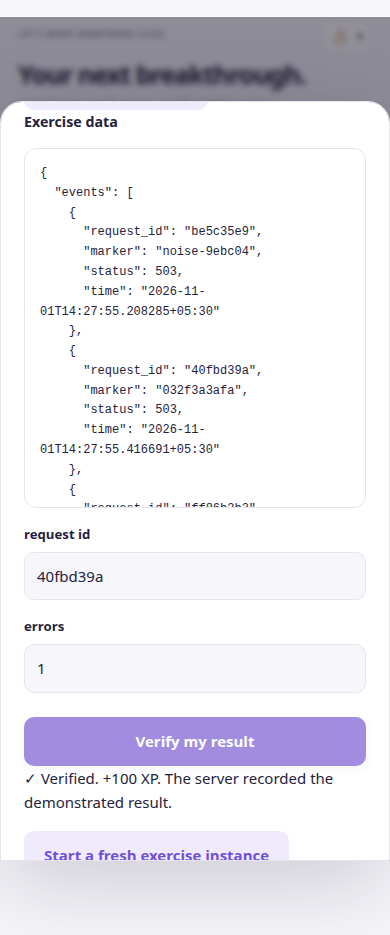
\includegraphics[width=.38\textwidth]{verified-lab-390.png}
\caption{Mobile browser integration: a generated logging result passes server verification. All displayed evidence and XP belong to a disposable test profile.}
\end{figure}

\section{Workspace UI: documentation, profile and reliable feedback}
\label{workspace-ui}
\subsection{Problems addressed}
The previous pack list exposed technical IDs and review/trust strings as its main
content, with the Read action on another line. Lesson actions sent their messages
to an ordinary page toast outside a native modal dialog; that toast was behind the
browser's top layer and often inaccessible to the learner. XP appeared only in
Stats, while profile settings were mixed into More. There was no in-app guide.

The refreshed interface uses a restrained learning-workspace pattern: neutral
surfaces, a clear text hierarchy, compact lists, one accent for actions/current
position, and additional semantic colors only for results, milestones and errors.
Today keeps one primary next step, an optional shorter task, and a milestone when
one is relevant. The path is a consistent vertical sequence. Advanced controls
are disclosed when needed. The design has not been scored by an independent
professional designer and makes no claim about a measured motivational benefit.

\subsection{Reference review and adaptation}
The review inspected Duolingo's official learning-path redesign article, the HTB
Academy public SOC path, GitHub Primer's button documentation, Material Design's
list guidance, the WAI modal-dialog pattern, MDN top-layer documentation, and
Nielsen Norman Group's progressive-disclosure guidance. The register in
\path{docs/design/ui-workspace-sources.json} records URLs, access results and limits.
TryHackMe returned HTTP 429; no authenticated or access-restricted interface was
claimed as inspected. Duolingo's article is a historical design explanation, not
an audit of every current app screen.

The useful patterns are a guided next lesson, explicit prerequisites and course
structure, predictable primary/secondary/quiet actions, consistently placed list
actions, and help near the point of use. Primer's component states and Material's
scannable lists inform the controls. WAI guidance informs modal focus and Escape
behavior. Ascend retains its own content, brand and constraints; third-party
screenshots and brand assets are not shipped as product assets.

\subsection{Navigation and information hierarchy}
The persistent top bar shows the verified XP balance, day streak and a profile avatar. The
balance and streak open Stats; the avatar opens Profile. Actual server totals update after
verification and on refresh. No additional coin currency, invented rank or
spendable balance is introduced. An unavailable balance is shown as a dash rather
than a fabricated zero. Documentation can load without a successful account fetch.

Five primary destinations are Today, Path, Stats, Tracks and Docs. Profile is
reached through the top bar. Existing \texttt{\#more} links continue to resolve to
Tracks. The profile route is \texttt{\#profile}; documentation supports topic links
such as \texttt{\#docs/timers}. Profile contains identity, earned totals, timezone,
appearance, reminders and privacy. Tracks contains mission controls, the library
and saved ideas. A reader need not scan account settings to find an installed pack.

\subsection{Component and interaction contract}
\begin{longtable}{P{.22\textwidth}P{.70\textwidth}}
\textbf{Component} & \textbf{Behavior and rationale}\\\hline
Top bar & Persistent XP, day streak and avatar; clear accessible names and real server totals. Narrow layouts may shorten or hide the context label, preserving actions.\\
Track picker & Choose a domain first, then one of its installed tracks. Changing domains clears the track choice; starting requires a selected track and no active mission.\\
Library row & Human title, supporting counts/review state and a right-aligned Read button. The title and action share one row. A long title truncates visually but retains its accessible text and full preview.\\
Library controls & Search installed packs; initially show eight rows in a large library, with Show all/Show fewer. Import controls and parked ideas use disclosures.\\
Pack preview & Complete title and tasks grouped by level, with the first group open. Mark reviewed does not complete tasks or grant execution trust.\\
Lesson dialog & Fixed close/header and feedback regions surround an independently scrolling body. Initial focus goes to the title for a lesson and to the first field for the short logging form. Escape closes; focus returns to the opener.\\
Action feedback & The live region moves into the active dialog. Error and in-dialog messages persist until dismissed or replaced. Page-level informational messages last eight seconds. Timer reminders cannot replace an unresolved error.\\
Buttons & One filled primary action, outlined secondary actions and quiet text actions. Pending actions disable repeat submission and expose an accessible busy state; a small spinner provides feedback. Disabled and selected states remain distinct.\\
Docs & Ten searchable help topics with stable links, readable prose, working command-copy actions, and related guides. The guide can be read offline after the shell is installed; progress writes still require the server.\\
Profile & Actual account identity and verified totals, editable timezone, locally persisted theme, reminders and opt-in streak sharing. Unsupported username/password editing is not presented.\\
Path & Uniform vertical task rows, current-level emphasis and distinct ready, locked, done, skipped and milestone states. Color supplements labels and shapes.\\
Typography & Locally bundled Inter Variable with its SIL Open Font License. A limited hierarchy separates headings, body copy and supporting labels; mobile form text is 16 px to avoid focus zoom.\\
Motion & Short 140--180 ms transitions and a pending-action spinner. The next challenge has a 1.8-second glowing border sweep on its first visible display after each page load; tab changes and data refreshes do not replay it. Reduced-motion preference disables decorative animation and transitions.\\
\end{longtable}

The palette is defined once using CSS variables for light and dark themes. Light
mode uses background \texttt{\#f7f8fa}, text \texttt{\#242a38}, supporting text
\texttt{\#626b7a}, and accent \texttt{\#5147c7}. Dark mode uses background
\texttt{\#15181f}, text \texttt{\#eceef4}, and accent \texttt{\#b2aaff}.
Cards, fields and buttons use a small, consistent corner-radius and spacing scale.
The saved theme is applied before first paint. Fonts and the help guide are
bundled locally; no third-party font request is required during use.

\subsection{Implementation and evidence}
The account-scoped pack-list endpoint now includes title, kind, level count, task
count and validity. It still excludes private filesystem paths, user IDs and
fingerprints. Invalid private pack content does not prevent the rest of the library
from loading. Loading changed content rechecks its review/trust state before
returning metadata. There is no schema migration or progress rewrite for this UI.

The in-app guide is structured content in \path{web/guide.json}; the documentation
builder generates the matching LaTeX chapter from the same content. The service
worker caches that guide, the local font and theme bootstrap together with the
application shell. Private API responses remain uncached. The standalone wheel
regression checks the guide, font/license and theme asset and serves them from an
installed wheel outside the source checkout.

The expanded automated suite records 146 passing tests. Browser regressions cover
inline pack-row geometry, readable previews, in-dialog failure messages, persistence
of errors, Escape/focus restoration, XP updates after verification, profile/theme/
timezone persistence, guide search and direct links, and offline help. The visual
audit captures the actual browser at 320, 390, 768 and 1440 px, including dark mode.
Axe-core 4.10.3 checks WCAG 2 A/AA and 2.1 AA tagged rules on thirty screen/viewport
combinations. Its results are bounded automated evidence, not a claim of complete
accessibility conformance or an expert usability score.

After the final typography and documentation-focus adjustments, all fifteen
browser/integration regressions passed again. The \texttt{ascend:ui-workspace}
image built successfully and passed the shipped hardened Compose configuration:
read-only root filesystem, non-root user, bundled guide/font/theme assets, native
grading, signed receipt checks, and XP persistence across container restart. This
runtime check used AMD64 and disposable data; the previous ARM64 compatibility
evidence does not constitute a new physical Raspberry Pi run.

The existing local server was restarted with its original command and environment
after creating a SQLite backup in the private profile. Health and pack metadata
checks passed. Before/after comparisons confirmed unchanged mission, entry, node,
unlock, evidence, lab, timer and XP records. No demonstration progress was added
to the real profile.

Retained evidence is in \path{docs/testing/ui-workspace-tests.txt},
\path{docs/testing/ui-visual-audit.txt}, \path{docs/testing/ui-accessibility.json}
and \path{docs/screenshots/ui-workspace/}. Final browser, container and local-refresh
records are in \path{docs/testing/ui-final-regressions.txt},
\path{docs/testing/ui-deployment-smoke.txt} and
\path{docs/testing/ui-local-refresh.txt}. All screenshots and scored examples use
a disposable account; no real learner progress is manufactured for the demonstration.
A useful independent review is to try choosing a track, finding its requirements,
starting a lesson, recovering from a failed check, locating XP/profile settings and
finding help, using both keyboard and phone input.

\begin{figure}[htbp]
\centering
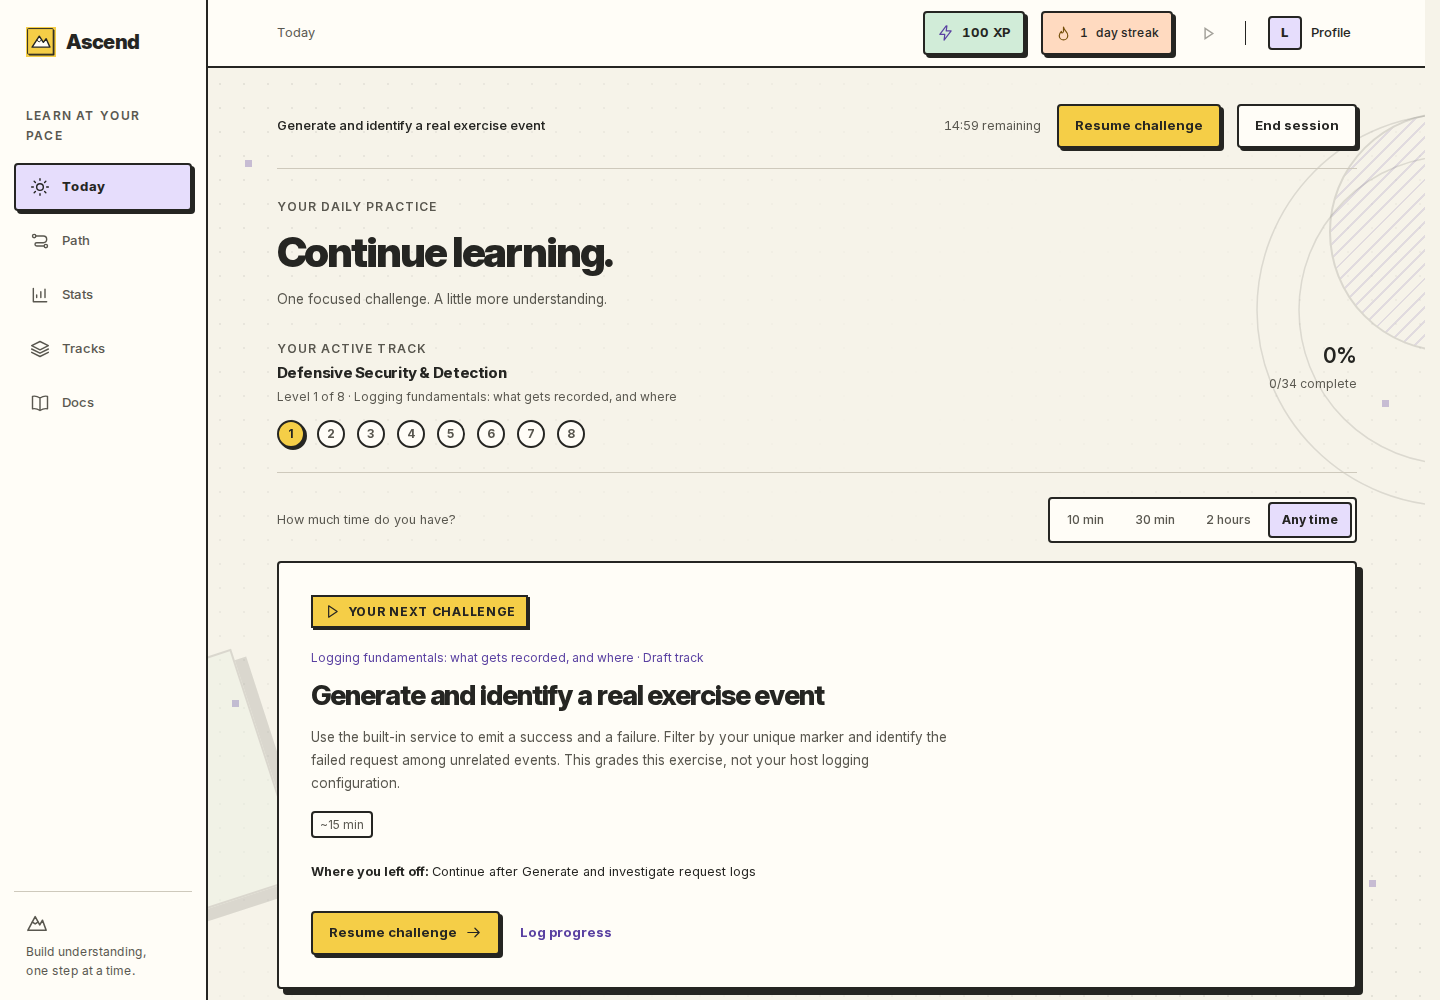
\includegraphics[width=\textwidth]{ui-workspace/today-desktop.png}
\caption{Current workspace: persistent XP/profile access, one primary learning action and restrained supporting content. Disposable demonstration account.}
\end{figure}
\begin{figure}[htbp]
\centering
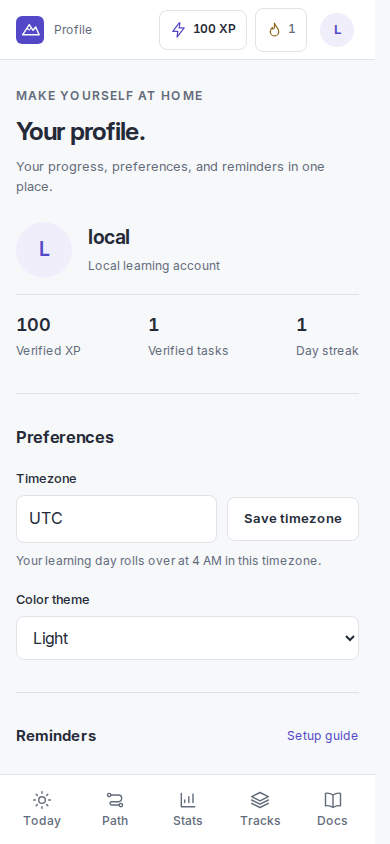
\includegraphics[width=.43\textwidth]{ui-workspace/profile-mobile.png}\hfill
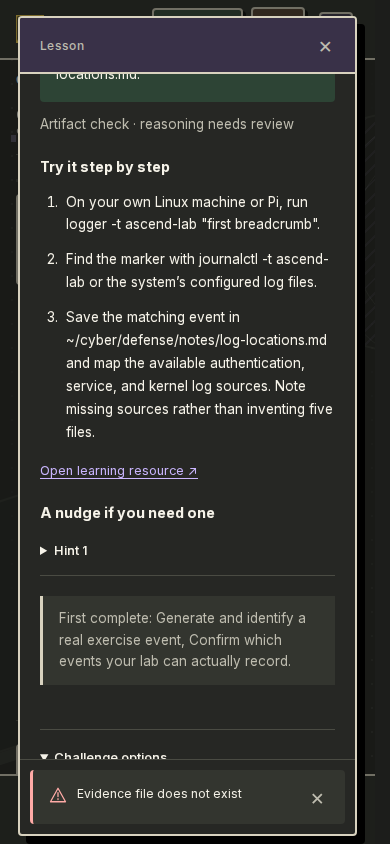
\includegraphics[width=.43\textwidth]{ui-workspace/lesson-feedback-mobile-dark.png}
\caption{Profile on mobile and visible feedback inside a dark-mode lesson dialog. These are viewport captures, not stitched page layouts.}
\end{figure}

\subsection{Independent Playground}
The approved short-practice design is implemented through its complete Playground
stage. Today retains the next track task alongside repeatable practice. Playground
contains seven worked examples, eighteen practice recipes, ten standalone challenges
and two editable browser workspaces across cybersecurity, Python and 3D reasoning.
Dedicated activity pages provide an elapsed practice clock and example-only
interactive walkthroughs. Skill-specific evidence and optional feedback inform recommendations;
case fixtures, saved work, hints and reveal history survive restarts. Activity
completion and capped rewards remain separate from curriculum completion and
legacy scored attempts. Authored checkpoints in selected long tasks record partial
learning without completing their parent. Desktop and phone flows, installed-wheel
assets and focused regression tests are checked using disposable profiles. See
\path{tests/test_playground.py} and \path{tests/test_playground_strict_timing.py}
for reproducible activity and timing checks. Further
learner sessions and the two-week observation window remain empirical follow-up.

\section{Architecture}
\begin{longtable}{p{0.23\textwidth}p{0.7\textwidth}}
\textbf{Component} & \textbf{Responsibility} \\
\hline
\texttt{ascend/engine} & Pure streak, pack, prerequisite, level, and validation rules. No subject-specific learning content. \\
\texttt{ascend/storage} & Scoped SQLite persistence, WAL connections, transactional numbered migrations. \\
Application layer & Shared use cases for logging, completion, missions, pack trust, corrections, and progress queries. \\
\texttt{ascend/cli} & Arguments, plain output, and an optional standard-library HTTP client. Remote mode never opens the local database. \\
\texttt{ascend/verifiers} & Local file and command adapters, HTTP/Git checks, and explicitly trusted extensions. \\
\texttt{ascend/server} & Optional FastAPI transport, account authentication, API contracts, static assets, and scheduled reminders. \\
\texttt{web} & PWA: Today, Path, Playground, Stats, Tracks, Docs and a top-bar Profile page. Same API and validation as the CLI. \\
\texttt{ascend/nudge} & Schedule decisions separated from delivery channels. \\
\end{longtable}

\section{Core rules and persistence}
The logical day rolls over at 04:00 in the user's timezone. Streaks are computed
from distinct logged days, never incremented counters. An isolated missing day
may bridge a chain once per ISO week; the freeze contributes zero days. Two
consecutive missing days break the chain. Today remains pending until rollover.
One acceptance-test row incorrectly counts a freeze as an extra day: the retained
reference algorithm and implemented test yield two logged days, not three.

Manual entries require at least twenty characters of learning and a next step.
Repeated learning text and recognizable passwords or challenge flags are rejected.
Partial work counts toward the streak; node completion is a separate decision.
Backfill adds historical node progress without manufacturing streak entries.
Main levels use milestone gates when available and otherwise require all steps;
side levels do not gate the main path. Conservative S/M/L time bounds are
30/120/240 minutes, with an optional more precise estimate.

Packs remain data, installed as private copies. Stable node identifiers preserve
progress across pack updates. Review and executable-code trust are independent,
content-bound decisions. SQLite migrations are applied in order, each in its own
transaction. Every business table is user-scoped from the first migration; the
server migration adds account and token tables without rekeying existing logs.

\section{Clients and interaction design}
The CLI's default view stays within six lines. It presents a mission, level,
next step, optional quick win, and streak status. The PWA now includes a dedicated guide and profile alongside its learning views. Today emphasizes a single next action, with a visually
secondary quick win. Path shows level groups, node states, and a separate side
lane. Stats exposes a heatmap, minutes, and note search. Tracks contains pack management; the top-bar avatar opens Profile for personal settings. Layouts are tested at mobile, tablet, and desktop
sizes. Theme preference is local to the browser.

The service worker caches static application assets only. Private API responses
are not cached. Offline writes are explicitly rejected; no background write queue
or conflict-resolution system is claimed. Editing and short-window undo retain
audit rows, and completion undo checks the node revision before reverting state.

\begin{figure}[ht]
\centering
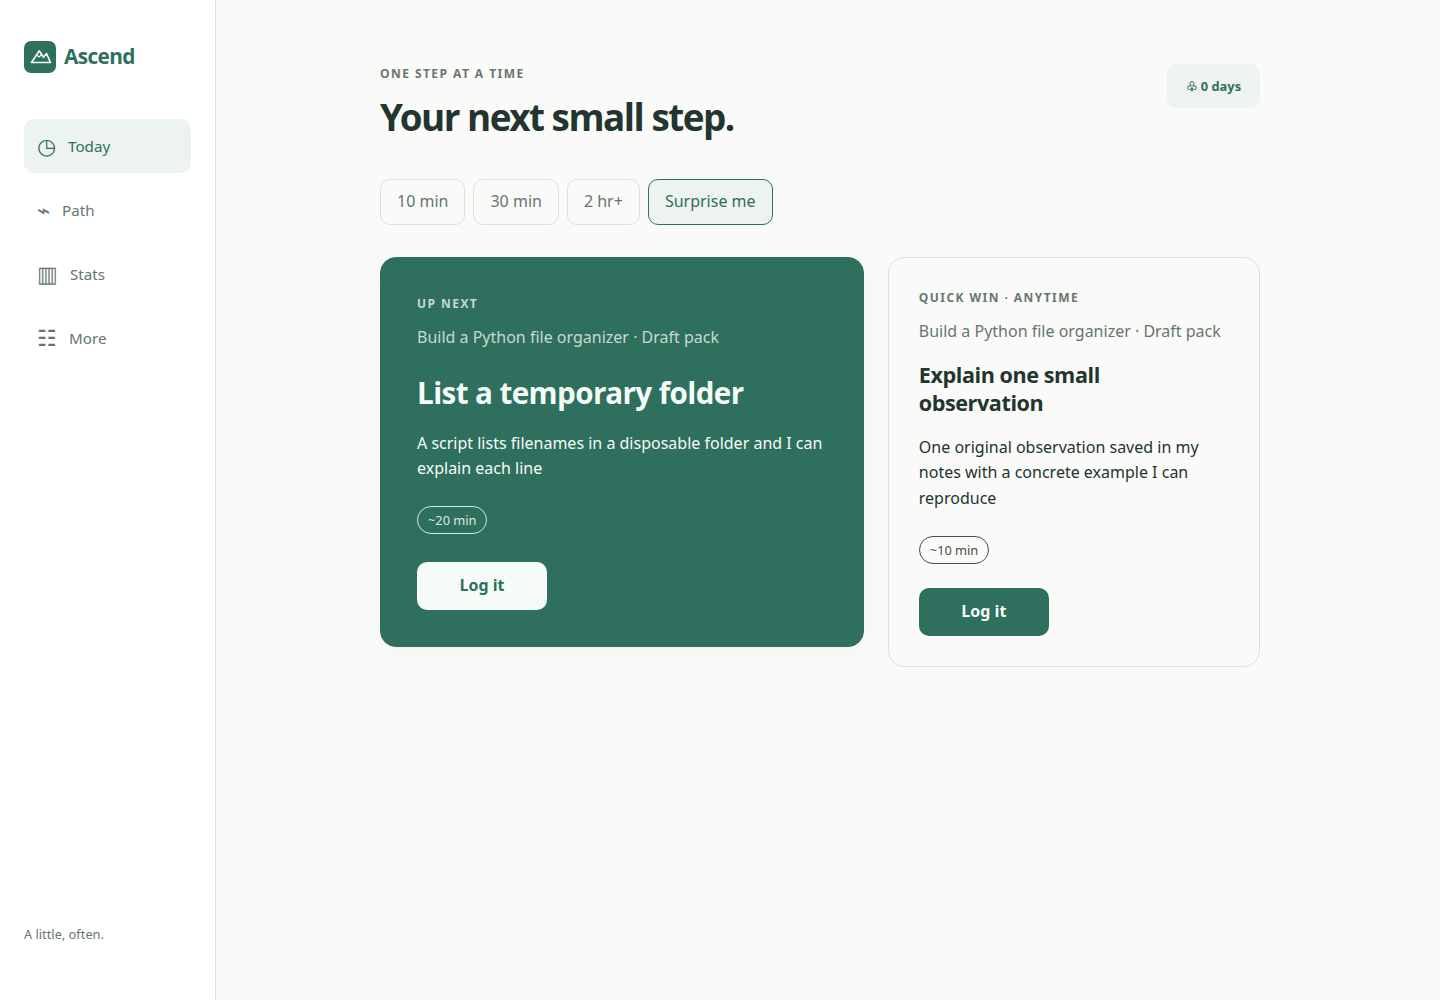
\includegraphics[width=\textwidth]{today-desktop.png}
\caption{Earlier Today design retained for comparison; the current workspace is shown in Section~\ref{workspace-ui}.}
\end{figure}

\section{Security boundaries}
Passwords use scrypt with random salts. API tokens are returned once and stored
as hashes on the server. CLI token files use mode 0600. Users' data is isolated by
scoped storage operations, and server logical dates use account timezones.
Accounts are administrator-created rather than openly registered.

Command verifiers execute argument arrays with \texttt{shell=False}, a ten-second
timeout, and no implicit \texttt{sudo}. Variables are substituted after splitting
the trusted template, so values cannot add arguments. Arbitrary command output
is not retained as evidence because it may contain secrets. Multi-user servers
restrict executable and network verifiers unless explicitly enabled by an
administrator; file checks are confined to the user's artifact directory.
Trusted plugins are code running with the host's permissions, not a security
sandbox. Network deployment should use TLS and an appropriate reverse proxy.

\section{Testing method}
The v1 and v2 acceptance tests were written before the implementation. Their
initial failing run is preserved alongside milestone results. Additional tests
cover input validation, pack updates, trust invalidation, proof timestamps,
notifications, account isolation, migrations, concurrent writes, and complete
browser logging flows. Every milestone runs the cumulative suite before its
implementation commit. Full command output is retained in \texttt{docs/testing/}.

The Phase 2 container smoke test found that editable source installs served the
PWA correctly while built wheels omitted its assets. A failing distribution
regression test was added first, then the build process was corrected to bundle
the canonical web and community sources. Both the installed wheel and container
now serve the PWA; the container also installs a bundled pack as UID 10001.

\section{Community distribution and extensions}
Phase 3 adds a bundled registry with SHA-256 digests, optional remote registries,
and explicit link checking with HEAD-to-GET fallback. Examples cover a home lab,
a Python file organizer, and a Blender still life. AI-authored examples remain
marked as drafts awaiting human review. Pack generation does not create lessons
or silently approve executable content. GitHub Actions runs the full suite and
lints every community pack across Python 3.11, 3.12, and 3.13.

Third-party verifier files are fingerprinted before trust, and their exact source
is checked again inside the worker before import. A changed file cannot execute
using an old trust decision. The worker's timeout and bounded result improve
failure handling but do not restrict trusted code's host permissions.

\section{Deployment and operational limits}
Standalone mode requires Python 3.11 or newer and no third-party runtime packages.
Server dependencies are optional extras. Docker uses a non-root runtime and a
persistent SQLite volume; Compose binds loopback by default. Profiles, tokens,
environment files, and user data are excluded from version control.

Automated tests do not establish that a real learning habit has lasted a week.
Android notification delivery requires a configured device/channel; real Web Push
also requires HTTPS and VAPID credentials. Browser and transport tests are reported
separately from live external delivery. No package registry publication or public
deployment is implied by a successful local build.

\section{Advanced notifications and public endpoints}
Phase 4 adds environment-configured Telegram delivery, authenticated webhooks,
and inline quick actions that collect learning text and a next step. Conversations
expire after twenty minutes, reject secrets, and deduplicate Telegram update IDs.
They record partial work through the shared application layer.

Web Push uses optional pywebpush dependencies for payload encryption and VAPID
authentication. Browser subscriptions are isolated per user; endpoint allowlists
prevent using the subscription API as an arbitrary HTTP client. Expired push
subscriptions are removed. The PWA requests permission only after an explicit
button click and supports unsubscribing the current browser. Public streak JSON
and SVG badges require a separate opt-in and expose no learning notes.

\section{Engagement refresh and curriculum assurance}
The completed engagement checkpoint added challenge briefs, hints, explicit partial/completion feedback, a connected level map, real milestone badges and revised cyber openings. The current curriculum revision strengthens all forty level assessments, adds prerequisites and later retrieval, and preserves existing task IDs. The full reasoning, evidence hierarchy, corrected assumptions, individual assessment rubric and unverified claims appear in the appended curriculum chapter. A file check still does not grade understanding.

The owner now requires LaTeX as the complete documentation reference and feature-sized commits. This report includes the complete operational and developer chapters; focused PDFs are also supplied. Historical Markdown inputs are preserved separately and are not the authoritative current contract.

\section{Reproduction}
\subsection{Historical version-3 curriculum and operations handoff}
All five private installed tracks were checked against the version-2 baseline,
backed up using SQLite's backup API plus pack-file copies, and upgraded through
the application to version 3. Entries, node states, missions, settings, split
tasks, level overrides and evidence history were compared before and after and
were unchanged. Review and executable trust remain unset. The running server
required no restart for this content update. Desktop and mobile browser checks
confirmed the new prerequisite, challenge dialog and Path without saving progress,
JavaScript errors or horizontal overflow. The sanitized record is
\path{docs/testing/curriculum-install.txt}; the actual backup stays outside Git.

The deployment guide's restore procedure was exercised with two disposable Docker
projects and synthetic data using the retained \texttt{ascend:phase4} image.
Binary tar streaming, volume ownership, SQLite integrity, progress records,
absolute pack paths, disabling both accounts' reminders, and the restored HTTP
health endpoint passed. This validates the restore procedure on the recorded
local image; it is not a new container-build, arm64 or external-notification test.
The image digest and result are in \path{docs/testing/restore-smoke.txt}.

The environment template and Compose mapping now document persistent auth mode
and notification settings. Host-code execution still defaults to disabled.
Compose rendering was checked with the example defaults and explicit auth,
host-code and push-provider overrides, without modifying any running service;
see \path{docs/testing/compose-config.txt}.
All seven LaTeX documents compile with generated CLI, schema and curriculum
references, with no missing glyphs, unresolved references or overflows above
one point. Representative rendered pages were inspected after fixing clipped
tables. Earlier Markdown design documents remain as historical source material.

\subsection{Build commands}
\begin{verbatim}
python3 -m venv .venv
.venv/bin/pip install -e '.[server,dev,push]'
.venv/bin/playwright install chromium
.venv/bin/pytest -v
.venv/bin/python scripts/update_report.py
.venv/bin/python scripts/build_docs.py
\end{verbatim}
The generated status section is refreshed after each milestone. The documentation builder compiles each LaTeX document twice and checks missing glyphs and unresolved references. XeLaTeX and the documented TeX packages/fonts are required.

\section{Handoff artifacts}
The complete CLI demonstration is saved in
\texttt{docs/testing/cli-demo.md}; it includes pack installation, mission start,
backfill, levels, default and time-filtered views, completion, statistics, and
the notification configuration/test commands. The demonstration uses synthetic
records in a temporary profile and a stub desktop notifier. It does not alter
the owner's real log or claim live desktop delivery.

The file tree is recorded in \texttt{docs/testing/file-tree.txt}. Container
build and smoke transcripts accompany the full pytest outputs. A separate
standalone-wheel smoke test installs the distribution into a new environment
without optional dependencies. Screenshots in \texttt{docs/screenshots/} show
the actual desktop and mobile layouts. All implementation commits use the
requested KDS-7Git author identity. The repository and release artifacts remain
local; no registry publication or external deployment has been performed.
\clearpage
\appendix
\section{User guide}
\subsection{Choose a way to use Ascend}
Use the standalone CLI for a local learning log with Python 3.11 or newer. Use the
server and browser for access from a laptop or phone. A remote CLI and the browser
share the server's data. They do not synchronize an independent local database.
For installation, Docker, HTTPS and account setup, see the deployment chapter.

A first standalone session from the repository root:
\begin{verbatim}
python3 -m venv .venv
.venv/bin/pip install -e .
source .venv/bin/activate
ascend pack install networking-for-security
ascend mission start networking-for-security
ascend
\end{verbatim}
Installed packs are private copies under the profile. The default profile is
\texttt{\textasciitilde/.config/ascend/}; set \texttt{ASCEND\_HOME} to choose another.
Bundled examples and cyber tracks are drafts. Read their tasks, set their lab
variables, and review them before trusting executable checks. Installation,
review, and trust do not execute lessons or provision a lab.

\subsection{The daily loop in the browser}
Today shows your active mission, main-path completion, one next challenge, and an
optional side challenge. Choose 10 minutes, 30 minutes, two hours, or any time.
Estimates are task estimates, not deadlines. A large task can take several logged
sessions. If nothing fits, open its Path details and split it into smaller
concrete steps, or choose a larger time budget.

Open challenge displays the scenario, finish line, any authored steps, a resource
link, and hints behind individual disclosures. The learning resource opens
outside Ascend; Ascend does not host lab machines. An older pack without guidance
fields still shows its original completion condition and resource.

Do the work, then choose Log progress. Record what you tried or learned and the
next action. Leave Mark as done unchecked for partial work. Check it only when the
finish line is met; configured evidence checks run on completion. A failed check
still saves the session and returns a reason, while leaving the challenge open.
Add details holds time spent and a proof reference. A proof reference does not
replace a required evidence file. The server must be able to access that file.

Path groups tasks by level, highlights the current position, and distinguishes
ready, locked, complete, skipped, and milestone nodes. Expand another level to
browse it; Jump to current level returns to your place. Challenge options expose
splitting, skipping, early unlocking, evidence checking, and reopening completed
or skipped work. Skipping is a navigation choice, not evidence of learning.

Stats shows streaks, active-day history, weekly minutes, searchable notes and
milestones completed in the active track. Skipped tasks do not earn these badges
or increase the browser's completed-step percentage. The legacy CLI level count
includes resolved (done or skipped) tasks, so it can differ from that percentage.
More contains missions, pack installation/upload, reminders, theme, parked ideas,
timezone, account and opt-in public streak settings. The keyboard shortcut
\texttt{L} opens logging when focus is outside an input. Escape closes a dialog.

\subsection{Evidence, progress and honest completion}
A file check confirms a file and optional size/pattern constraints. It does not
read your reasoning or grade mastery. Manual checks rely on your confirmation.
Command, HTTP, Git and plugin checks have their documented technical scope;
none independently certifies professional competence. The curriculum chapter
specifies stronger human assessment criteria for the cyber milestones.

Keep flags, passwords, tokens and personal information out of notes. The secret
guard rejects recognizable patterns, but is not a general data-loss-prevention
system. Keep sanitized evidence locally and log its path or a permitted reference.

\begin{verbatim}
ascend done "I compared the successful request with a refused connection" \
  "Check which layer failed" --minutes 20
ascend done "I reproduced and explained the required result" \
  "Try the changed case" --node PACK:NODE --complete
ascend check PACK:NODE
\end{verbatim}
Replace \texttt{PACK:NODE} with a real node reference. To inspect IDs, use
\texttt{ascend levels --json}. Explicit manual marking and force overrides remain
available in the CLI/API; record a reason and do not interpret an override as a
successful verifier or assessment.

\subsection{Missions, other tracks and returning after a break}
Only one mission is active. Pause it before starting another track. Starting a
pack makes a new mission record; task progress belongs to the pack and survives
switches. Finish is an explicit mission lifecycle action; it does not certify
that every node was independently assessed.
\begin{verbatim}
ascend mission pause
ascend mission start defensive-security-and-detection
ascend mission list
ascend mission nudge-time 20:30
ascend mission nudge-time off
\end{verbatim}
Save an unrelated idea using \texttt{ascend park "idea"} or More. Resolve it when
appropriate. Backfill records work completed before using Ascend without adding
streak days. Return to an old challenge to practice again or use the version-3
return-later checks after a few days. Their suggested interval is not scheduled
or enforced by the engine.

\subsection{Corrections, history and exports}
Use \texttt{ascend edit ID --learned "corrected explanation" --next-step "action"}
to fix an entry. \texttt{ascend undo} reverses the most recent entry only within
its ten-minute window; a node revision check protects newer completion changes.
Use \texttt{ascend search "phrase"}, \texttt{ascend stats}, and
\texttt{ascend export log.md}. Export is a readable Markdown learning log, not a
complete account/database backup. The backup procedure is in the deployment guide.

\subsection{Streaks, reminders and phone access}
A logical day rolls over at 04:00 in the configured IANA timezone. Distinct logged
days count, including partial work. One isolated gap can be bridged per ISO week;
a freeze adds no logged day, and two consecutive missing days break the chain.
Today remains pending until rollover. Backfilled task status does not add a day.

Reminders are opt-in in server mode. Choose a channel, configure it, send an
explicit test, and enable reminders. The active mission's time overrides the
global time. The scheduler stops after a log and sends at most two successful
scheduled reminders per logical day. True device delivery requires a real channel
and device; a passing transport test does not establish it. The notifications
chapter covers ntfy, Telegram and Web Push fully.

For Android, open the HTTPS-served app and use the browser's installation option
when available. API responses are never cached. Reconnect before saving; no
offline write queue or conflict resolution is implemented.

\subsection{Pack updates and troubleshooting}
Compare an update with \texttt{ascend pack diff file.toml}, back up local edits,
and install it. Stable task IDs preserve existing completion and skips. Changed
content resets review and execution trust. Version-3 assessments do not
retroactively certify work completed under an older definition. Complete the new
return-later checks or reassess a milestone if you want evidence under the new rubric.

If no task appears, check the active mission, time filter, prerequisites, level
gates and whether the main path is resolved. If a resource fails, use its official
course index and report the link; do not guess a substitute solution. If a file
check fails, check the expanded path on the machine doing verification. A laptop
file is not automatically present in a server container. In restricted multi-user
mode, evidence must lie in the account's allowed artifact directory. If the UI is
stale after an upgrade, reload it; the service worker updates the shell while
keeping API data uncached. If a lesson requires unsupported hardware, use a
supported lab environment instead of weakening the learning objective.

% Canonical LaTeX chapter; migrated from docs/deployment.md.
\hypertarget{deployment}{%
\section{Deployment and operations}\label{deployment}}

From an existing repository checkout, prepare the local server environment:
\begin{verbatim}
python3 -m venv .venv
.venv/bin/pip install -e '.[server,push]'
source .venv/bin/activate
ascend-server
\end{verbatim}
The default bind is \texttt{127.0.0.1:8420}.
To serve your LAN, bind the machine\textquotesingle s specific LAN
address. \texttt{-\/-host 0.0.0.0} is explicit and prints a reminder to
use a TLS reverse proxy beyond your trusted LAN. Multi-user deployments
are for administrator-provisioned accounts, not anonymous public signup.
Single mode has no login. Use multi mode even for one person when the service
is reachable by people who should not have access to the learning profile.

\begin{verbatim}
ascend-server user-add alice --timezone Asia/Kolkata
AUTH_MODE=multi ascend-server
\end{verbatim}

Every account needs an IANA timezone. Existing standalone data remains
with the implicit \texttt{local} account (ID 1). In multi-user mode that
account has no password and cannot log in. Create real accounts for
separate users; switching auth mode does not transfer the local
profile\textquotesingle s data into a newly created account.

\hypertarget{docker-linux-pc-vps-or-raspberry-pi}{%
\subsubsection{Docker: Linux PC, VPS, or Raspberry
Pi}\label{docker-linux-pc-vps-or-raspberry-pi}}

\begin{verbatim}
cp -n .env.example .env
chmod 600 .env
docker compose -f docker/docker-compose.yml up -d --build
\end{verbatim}
Run Compose commands from the repository root so they load the same \texttt{.env}.
From another directory, supply \texttt{--env-file /absolute/path/to/.env} as well
as the Compose file. Edit that private file to persist auth mode and notification
credentials across restarts; do not rely on a one-command environment override
for a lasting deployment setting. \texttt{cp -n} preserves an existing file.
Compose forwards the variables listed in its environment mapping; an arbitrary
new variable in \texttt{.env} is not automatically passed into the container.

The Python slim base supports amd64 and arm64. The image uses UID 10001
and a named persistent \texttt{/data} volume. Compose maps the service
to loopback; put Caddy or another TLS reverse proxy in front of it. A
minimal Caddy configuration is:

\begin{verbatim}
ascend.example.com {
    reverse_proxy 127.0.0.1:8420
}
\end{verbatim}

Replace the domain and configure DNS before deployment. Android PWA
installation and Web Push require a secure origin. Proxy requests
preserve their original host so the server can validate same-origin
browser writes.

If container builds cannot reach PyPI, prepare wheels on the host:

\begin{verbatim}
python3 -m pip wheel --no-build-isolation -c docker/constraints.txt \
  --wheel-dir docker/wheelhouse '.[server,push]' setuptools wheel
docker build --build-arg ASCEND_OFFLINE=1 -f docker/Dockerfile -t ascend:local .
python scripts/container_smoke.py ascend:local
\end{verbatim}

The ignored wheel cache is used only when explicitly enabled with the build argument
\texttt{ASCEND\_OFFLINE=1}. Generate that cache for the target Python version and
architecture; laptop AMD64 wheels must not be reused as Pi ARM64 wheels. Normal
builds download pinned dependencies. Wheels are not copied into the runtime image
or committed. Actual arm64 execution still needs verification on arm64 hardware.

\hypertarget{reminders}{%
\subsubsection{Reminders}\label{reminders}}

Set ntfy as the channel, choose a long private topic, subscribe in the
Android ntfy app, send a test, and enable reminders. Environment
\texttt{NTFY\_SERVER} defaults to \texttt{https://ntfy.sh}; optional
\texttt{NTFY\_TOKEN} stays in the environment. Each account can store a
separate topic. Server scheduling checks every thirty seconds and uses
the user\textquotesingle s logical day and mission override. It sends at
most two successful scheduled reminders per day and stops after logging.
Test sends are explicit and do not consume daily schedule slots. A
second reminder occurs two hours after the first; schedules close to
rollover may have only one reminder that day.

\hypertarget{trust-and-backups}{%
\subsubsection{Trust and backups}\label{trust-and-backups}}

Multi-user deployments restrict command, plugin, Git, and HTTP verifiers
by default. \texttt{ASCEND\_ALLOW\_CODE=1} is an administrator opt-in to
host-code execution after each user\textquotesingle s explicit trust;
enable it only for users you trust with host permissions. Restricted
file checks use
\texttt{/data/artifacts/\textless{}user-id\textgreater{}/}.

Back up SQLite using its backup API rather than copying a live WAL
database:

\begin{verbatim}
python -c "import sqlite3; s=sqlite3.connect('/data/ascend.db'); d=sqlite3.connect('/backup/ascend.db'); s.backup(d); d.close(); s.close()"
\end{verbatim}

Also back up private packs and plugin files. Installed pack records contain
absolute paths: a container restore should retain the internal \texttt{/data}
path; a local restore needs the same profile path or an explicit path migration.
Migrations run on startup in numbered
transactions. Newer schemas should not be opened with an older
application release.

\subsection{Container accounts, upgrades and a recoverable backup}
Use the same Compose file for administration so the command targets the existing
named volume. Provision a multi-user account before switching authentication mode:
\begin{verbatim}
docker compose -f docker/docker-compose.yml exec ascend \
  ascend-server user-add alice --timezone Asia/Kolkata
AUTH_MODE=multi docker compose -f docker/docker-compose.yml up -d
\end{verbatim}
Also set \texttt{AUTH\_MODE=multi} in the private \texttt{.env} before future
recreation, or the default could switch the server back to single mode.
A mode switch does not copy the implicit local account into Alice. Do not use
\texttt{down -v} for an ordinary upgrade; it removes the persistent volume.

For a simple consistent container backup, stop the service, copy the complete
profile volume through a temporary container into a protected host directory,
then restart. A named backup directory avoids accidental overwrite:
\begin{verbatim}
umask 077
mkdir -m 700 backup-YYYYMMDD
docker compose -f docker/docker-compose.yml stop ascend
docker compose -f docker/docker-compose.yml run --rm --no-deps -T \
  --entrypoint tar ascend -C /data -czf - . > backup-YYYYMMDD/profile.tar.gz
docker compose -f docker/docker-compose.yml start ascend
\end{verbatim}
The shell creates the archive as the current host user; restrict its permissions
and store it outside the repository. Stopping avoids copying an inconsistent
live WAL database. The SQLite backup API shown earlier is appropriate for an
online database snapshot, but packs, plugins and persistent keys need coordinated
backup too. Never print secrets to verify a backup.

Test restoration into a \emph{new}, isolated volume. Keep the original
untouched until health checks, login, entry counts, a known pack and its progress
are verified. Restore the complete profile, including keys needed for existing
subscriptions, and preserve ownership for container UID 10001. Run the matching
application version first. Only promote the restored profile after validation.
There is no automatic rollback to an older database schema.

\subsection{An isolated container restore drill}
Run these commands from the repository root, replacing the backup directory with
the one just created. Save the exact image before upgrading; its immutable image
ID selects the application version for the drill. These examples require Docker
Compose v2. Keep a protected copy of external environment credentials separately;
they are not included in the profile archive.
\begin{verbatim}
export ASCEND_RESTORE_IMAGE="$(docker compose -f docker/docker-compose.yml images -q ascend)"
test -n "$ASCEND_RESTORE_IMAGE"
docker image save "$ASCEND_RESTORE_IMAGE" > backup-YYYYMMDD/image.tar
cat > backup-YYYYMMDD/restore.compose.yml <<'YAML'
services:
  ascend:
    image: ${ASCEND_RESTORE_IMAGE:?set the backed-up image ID}
    ports:
      - "127.0.0.1:8421:8420"
    volumes:
      - restored-data:/data
    environment:
      AUTH_MODE: ${ASCEND_RESTORE_AUTH:-single}
volumes:
  restored-data:
YAML
docker compose -p ascend-restore -f backup-YYYYMMDD/restore.compose.yml \
  run --rm --no-deps -T --entrypoint tar ascend \
  -C /data -xzf - < backup-YYYYMMDD/profile.tar.gz
\end{verbatim}
Use a previously unused project name if \texttt{ascend-restore} already exists.
Do not overlay an old restore volume. On another host, load \texttt{image.tar}
with \texttt{docker image load} and select the loaded image. The new volume has
the same internal path and UID as production but a different Compose identity.

Before starting the restored server, disable scheduled notifications in every
restored account. This changes only the copy and prevents duplicated reminders:
\begin{verbatim}
docker compose -p ascend-restore -f backup-YYYYMMDD/restore.compose.yml \
  run --rm --no-deps -T --entrypoint python ascend - <<'PY'
from ascend.storage import Database
db = Database()
ids = {1} | {r[0] for r in db.connection.execute("SELECT id FROM users")}
assert db.connection.execute("PRAGMA integrity_check").fetchone()[0] == "ok"
for user_id in ids:
    db.user_id = user_id
    db.set_setting("nudge_enabled", False)
for table in ("entries", "missions", "packs", "node_state"):
    print(table, db.connection.execute("SELECT count(*) FROM " + table).fetchone()[0])
db.close()
PY
# Use multi for a production profile that used provisioned accounts.
export ASCEND_RESTORE_AUTH=single
docker compose -p ascend-restore -f backup-YYYYMMDD/restore.compose.yml up -d
curl -fsS http://127.0.0.1:8421/api/health
\end{verbatim}
Compare these table counts with a read-only query on the backup database. Open
port 8421, verify the matching authentication mode, a known mission, evidence path
and completed node, and check the container logs. Do not make practice entries in
the production profile. Health and integrity checks alone do not establish that
all application data and external integrations were restored correctly.

After validation, stop the drill with the same \texttt{-p ascend-restore} and
\texttt{-f} options followed by \texttt{down}. Keep its volume until satisfied;
volume deletion is an explicit cleanup step, never part of a normal upgrade.
For real recovery, stop the damaged deployment first, restore into a fresh
production volume at \texttt{/data}, verify it in isolation, then change the
proxy/port to it. Re-enable reminders only on the promoted instance and restore
its external credentials. A rollback requires the matching pre-upgrade database
and image; merely changing an image tag does not undo a migration.

\subsection{Routine upgrade and readiness checks}

\begin{verbatim}
docker compose -f docker/docker-compose.yml up -d --build
curl -fsS http://127.0.0.1:8420/api/health
docker compose -f docker/docker-compose.yml logs --tail=100 ascend
\end{verbatim}
A successful health response establishes process/API readiness, not working
external notifications or lab connectivity. Build on the target architecture for
a simple Pi deployment. The base image supports arm64; this is distinct from a
claim that every optional external training tool supports it. The local server
can be restarted after Python changes; static asset changes are picked up on
reload, and new pack text still has to be installed into private copies.

% Canonical LaTeX chapter; migrated from docs/notifications.md.
\hypertarget{notifications-and-public-streaks}{%
\subsection{Notifications and public
streaks}\label{notifications-and-public-streaks}}

Reminders are opt-in on the server. Configure them in \textbf{Profile →
Reminders} or with \texttt{ascend config nudge-enabled true}. First
test the chosen channel. The server owns the log and schedule; clients
do not mirror the database.

\hypertarget{ntfy}{%
\subsubsection{ntfy}\label{ntfy}}

The default server channel is ntfy. Subscribe to a long private topic
using the ntfy Android app, set
\texttt{ascend config ntfy-topic \textless{}topic\textgreater{}}, and
choose \texttt{ascend config nudge-channel ntfy}.
\texttt{NTFY\_SERVER} may point to your own instance;
\texttt{NTFY\_TOKEN} is read only from the environment. Public hosted
topics are known by their names, so use a random topic and do not put
secrets in reminders.

\hypertarget{telegram-and-inline-quick-actions}{%
\subsubsection{Telegram and inline quick
actions}\label{telegram-and-inline-quick-actions}}

Set \texttt{TELEGRAM\_BOT\_TOKEN} and \texttt{TELEGRAM\_CHAT\_ID} in the
server environment, then select
\texttt{ascend config nudge-channel telegram}. Credentials are never
stored in SQLite. For multi-user servers, the administrator maps each
account using
\texttt{TELEGRAM\_CHAT\_ID\_\textless{}numeric-user-id\textgreater{}}.
Only configured private chats are accepted.
For Compose, add each per-user mapping explicitly under the service's environment
section, for example \texttt{TELEGRAM\_CHAT\_ID\_2: \$\{TELEGRAM\_CHAT\_ID\_2\}},
and define its value in the private environment file. Unlisted keys in that file
are not automatically forwarded to the container.

Reminders include \textbf{Log a step} and \textbf{Log quick win}
buttons. Tapping a button starts a twenty-minute conversation: what you
learned (minimum 20 characters), then your next step. Both fields go
through the shared secret guard and entry validation. The result is a
partial learning entry, not an automatic node tick. \texttt{/cancel}
abandons the conversation. Telegram update IDs prevent duplicate logs
when webhook deliveries are retried.

For buttons to work, expose the server through HTTPS and register
\url{https://your-domain/api/telegram/webhook} with
Telegram\textquotesingle s \texttt{setWebhook} method, including a
random \texttt{secret\_token} matching the server\textquotesingle s
\texttt{TELEGRAM\_WEBHOOK\_SECRET}. See
\href{https://core.telegram.org/bots/api\#setwebhook}{Telegram\textquotesingle s
official Bot API}. \texttt{ASCEND\_PUBLIC\_URL} supplies the optional
Open Ascend button. Missing bot/chat credentials fall back to desktop
with a warning recorded once; a headless server reports the unavailable
desktop transport explicitly.

\hypertarget{web-push-no-separate-android-app}{%
\subsubsection{Web Push: no separate Android
app}\label{web-push-no-separate-android-app}}

Install the optional dependency and generate a persistent VAPID key
pair:

\begin{verbatim}
pip install '.[server,push]'
ascend-server push-keys --out /your/private/ascend/vapid.pem
\end{verbatim}

The command writes the private key with mode 0600 and prints only the
public key. Set \texttt{VAPID\_PRIVATE\_KEY} to the private
file\textquotesingle s path and \texttt{VAPID\_SUBJECT} to a
\texttt{mailto:you@example.com} contact or an HTTPS contact URL. The
Docker image includes the Push extra; generate the key as the container
user under \texttt{/data/} so it persists in the volume. Key generation
refuses to overwrite an existing file.
For the default Compose volume, generate it with:
\begin{verbatim}
docker compose -f docker/docker-compose.yml exec ascend \
  ascend-server push-keys --out /data/vapid.pem
\end{verbatim}
Persist the subject and public app URL in the private environment configuration,
then recreate the service so the new environment takes effect. Do not regenerate
an existing private key as an ordinary upgrade step.

Serve the PWA over HTTPS. In Profile, choose \textbf{Enable browser
notifications}, grant permission, enable reminders, and send a test.
Subscriptions belong to the logged-in account. The service worker
displays encrypted push payloads and opens the app when tapped. Disable
on this browser removes only that browser\textquotesingle s
subscription.

The server validates HTTPS push-service endpoints and subscription keys,
uses pywebpush for standard encryption and VAPID authentication, and
removes expired 404/410 subscriptions. Common Chrome, Firefox, and Apple
provider hosts are accepted. An administrator can add exact providers
with \texttt{PUSH\_ALLOWED\_HOSTS}.

Automated verification covers actual payload encryption and VAPID
headers while mocking the final HTTP transport. It does \textbf{not}
establish real Android delivery: that needs your own domain, keys,
notification permission, and subscribed device.

\hypertarget{opt-in-public-streak-and-badge}{%
\subsubsection{Opt-in public streak and
badge}\label{opt-in-public-streak-and-badge}}

\texttt{ascend config public-streak true} (or Profile → Share my streak
publicly) exposes:

\begin{itemize}
\tightlist
\item
  \texttt{/api/public/\textless{}username\textgreater{}/streak}: current
  and best streak plus today\textquotesingle s logged flag.
\item
  \texttt{/api/public/\textless{}username\textgreater{}/badge.svg}: an
  embeddable SVG badge.
\end{itemize}

These routes return 404 until enabled. They never include entries,
proof, private packs, mission names, or learning notes. Set the option
back to false to withdraw access. The implicit standalone/single-server
username is \texttt{local}.

\section{Developer handbook}
\subsection{Architecture and boundaries}
The engine owns pure rules: TOML parsing, dependency/level eligibility, streaks,
and validation. Storage owns SQLite migrations and user-scoped access. The
\texttt{Tracker} application layer implements shared use cases. CLI and FastAPI
are transports over those use cases; the vanilla JavaScript PWA consumes the API.
Subject content belongs in packs, not engine conditionals. Verifier adapters own
external effects and return bounded, sanitized evidence results.

Key files: \texttt{ascend/engine/packs.py} defines immutable Pack, Level and Node
models; \texttt{levels.py} computes candidates; \texttt{streak.py} derives streaks;
\texttt{ascend/application.py} coordinates use cases;
\texttt{ascend/storage/\_\_init\_\_.py} scopes storage;
\texttt{ascend/server/app.py} declares HTTP routes and security headers;
\texttt{ascend/cli/remote.py} implements standard-library remote access;
\texttt{web/app.js} and \texttt{web/style.css} own interaction and presentation.

\subsection{State and data flow}
A pack install parses and validates before replacing the private text file and
recording its content fingerprint. Stable IDs join task state to pack data.
Loading a changed file revokes stale review/trust. User variable settings are
applied separately from authored placeholders. A task split creates application
nodes while keeping the pack file unchanged. Prerequisites and main-level gates
control recommendations; explicit overrides are logged as overrides.

Logging resolves an account/mission/node, validates learning text, optionally runs
a verifier, then records the session in a transaction. Failed completion still
records partial work. Successful completion records its prior state and revision
so undo can avoid clobbering a later change. Streaks and time statistics are derived
from entries, not independent mutable counters. File/Git evidence timestamps can
be backdated to actual work time and are deduplicated by the existing evidence flow.

\subsection{Challenge preview and started workspace}
\path{ascend/server/presentation.py} removes instructions, downloads, hints,
completion criteria and verifier internals from web overview and
listing responses, including the current level nested in the dashboard response.
Resource links, labels and notes remain available before Start so learners can
prepare without starting the timer. \texttt{preview} and \texttt{requirements} are authored Node fields with the usual
variable and series substitutions. Older packs can omit them and show a title.
The challenge route returns full content only when the current user has a task
session or historical completion. A direct URL cannot skip the preview; an ended
session retains review access. Public pack exports and the standalone CLI remain
authoring/practice tools, so this is not an anti-cheat secrecy boundary.

In \path{web/app.js}, \texttt{showNode} builds either the short preview or the full
workspace. Start creates the existing server-clock session and navigates to the
challenge route; opening or reviewing a preview does not create a session. Reload
and Review attempt reuse existing state. No pause or timer reset is introduced.
API regression tests exercise nested/list responses and review access; browser
tests cover direct links, downloads, copyable commands and timer restoration at
mobile and desktop widths.

\subsection{Security and operational assumptions}
Every business query is user-scoped. Passwords use scrypt and server bearer tokens
are hashed. CLI token storage uses restrictive permissions; browser tokens are
session-scoped unless the learner chooses Remember me. The PWA uses DOM text construction for authored content. The server
sets a self-only content security policy, same-origin write checks and no-store
headers for API responses. Signup is opt-in in multi-user mode and has a bounded
per-process creation limit. One-use recovery codes rotate atomically and revoke
earlier tokens. Public-production limits remain those documented for the chosen
deployment topology. The public catalog never reads private installed packs.

Command templates are split before substitution and run without a shell. Plugins
run in a separate process with a timeout, but retain the host user's permissions.
Multi-user executable/network checks are restricted unless the administrator opts
in. Do not infer sandboxing from process isolation or from pack validation. The
verifier chapter gives the exact extension contract.

\subsection{Build, test and contribution loop}
Install Python 3.11 or newer and its virtual-environment support. Documentation
builds use XeLaTeX, the extra LaTeX packages and DejaVu fonts. On Debian/Ubuntu,
the documentation prerequisites can be installed with:
\begin{verbatim}
sudo apt-get install texlive-xetex texlive-latex-extra fonts-dejavu
\end{verbatim}
Pandoc was used for the one-time migration of historical Markdown; it is not
needed for routine builds or edits to the canonical LaTeX chapters.
\begin{verbatim}
python3 -m venv .venv
.venv/bin/pip install -e '.[server,dev,push]' setuptools wheel
.venv/bin/playwright install chromium
.venv/bin/pytest -v
.venv/bin/ruff format --check ascend tests scripts setup.py
.venv/bin/ruff check --select F401,F841 ascend tests scripts setup.py
.venv/bin/python scripts/build_registry.py
.venv/bin/python scripts/build_docs.py
\end{verbatim}
Tests use temporary profiles and local test servers. They cover pure rules,
application semantics, CLI/remote behavior, account isolation, migrations,
notifications, browser flows and built-wheel assets. Add meaningful regression
coverage for a behavioral change; do not run external lab attacks in the test
suite. Resource link checks are explicit network operations, separate from offline
unit tests. The CI matrix covers Python 3.11--3.13.

With an already built local image, run the optional operations drill:
\begin{verbatim}
.venv/bin/python scripts/restore_smoke.py ascend:local
\end{verbatim}
It creates two disposable Compose projects, backs up a synthetic profile, restores
it at the same internal path, runs the guide's exact reminder-disable program,
checks data and HTTP health, then removes only its own test volumes. It does not
send notifications or touch the production profile. The retained result names
the exact image tested; it is not an arm64 or external delivery check.

The \texttt{setup.py} build hook copies canonical \texttt{web/} and
\texttt{packs/community/} assets into wheels. Verify installed artifacts as well
as editable installs. \texttt{scripts/screenshots.py} uses disposable illustrative
data, not the owner's profile. Never commit databases, credentials, environment
files, personal logs, or real deployment addresses. Make feature-sized commits
and update the implementation report at each milestone.

\subsection{Maintaining the curriculum and documentation}
Canonical runtime learning content is TOML under \texttt{packs/community/}.
Files are grouped into \texttt{foundations/}, \texttt{offensive/},
\texttt{defensive/}, \texttt{engineering/}, \texttt{specialist/},
\texttt{practice/}, and \texttt{projects/}. The registry records each relative
path so installation by pack ID remains independent of the folder layout.
The exported cyber pack files must match it. Preserve IDs, increment pack version,
regenerate registry checksums, validate the dependency graph, and document revised
completion requirements. The assessment map in
\texttt{docs/curriculum/assessment-map.json} records one explicit mechanism,
experiment, transfer case, control and delayed-retrieval prompt for each main
level. Source evidence, access dates and limits are in
\texttt{docs/curriculum/sources.json}. Keep both synchronized with the authored
milestones; the curriculum regression suite checks their structural contract.

The canonical narrative documentation is LaTeX under \texttt{docs/latex/}.
\path{scripts/build_docs.py} refreshes generated command/schema/curriculum
appendices and compiles the report, complete handbook and focused guides.
Generated sections are marked as such. Edit narrative chapters directly; do not
regenerate them from legacy Markdown. The remaining Markdown documents are
convenience copies or historical inputs. Command documentation may be duplicated
there, but the LaTeX reference is complete. Historical designs are separately
compiled and explicitly labeled as superseded, never mixed with current guidance.

\subsection{Schema and extension contracts}
The pack-format and verifier chapters specify all authored fields and extension
boundaries. The API chapter combines a human-readable endpoint reference with
request-model information extracted from OpenAPI. The generated storage appendix
reproduces the numbered migration sources used by the running code. Migrations
are sequential transactions over a WAL-backed database; do not open a newer
schema with an older binary. Change shared semantics in the application layer and
check both standalone and remote callers before release.


\subsection{Linux local labs and bounded grading}
\path{ascend/local_labs/catalog.py} is the separate reference and recipe catalog
shared by tracks, the Linux labs tab and CLI. The research register is published
with \path{scripts/build_lab_catalog.py}; packaged runtime data lives in
\path{ascend/local_labs/resources}. Adding a reference never activates an adapter.
Recipe activation requires immutable downloads, reviewed code, versioned checks,
platform measurements and lifecycle evidence. The HTTP command gateway rejects
client-only runtime operations, even on a single-user server.

Migration 0011 adds account/nonce/version-bound external lab attempts and the
foreground-session guards. Migration 0012 adds assigned policy cases. Local run
state, download cache and saved work are separate and bound to the local profile;
the API cannot launch the companion or read a submitted local path. The Docker
adapters inventory resources before provisioning, verify ownership labels,
enforce internal target networks and loopback proxies, retain failed cleanup
state and reconcile after process interruption. Source/image eviction is scoped
to acquired, unused objects; user work is retained.

\path{ascend/local_labs/prefix_worker.py} is a fixed, data-only IPv4 policy
checker invoked with isolated Python startup in a temporary directory. It
accepts at most 64 KiB and 32 declarative rules, with Linux CPU, address-space,
process, descriptor, output and wall-clock limits. The parent checks its pinned
hash, output version and complete checkset and reaps failures. Partitioning route
indices at every rule boundary proves equivalence over the supported policy
language; this is not a general sandbox for executable submissions. Online cases
are server-issued; offline case keys derive a canonical case on the server.
Source, recipe, checker, worker hash and case bind the fixture identity.

\path{ascend/local_labs/upstream.py} adapts selected Labtainers/netlab report
semantics and strict specialist observation templates without launching those
providers. Empty goals and unsupported/warning exits never become passing
grades. Manual observations stay explicitly manual, including claimed environment
hashes and model trial counts. Temporary server policy tests and local reports
issue no track proof or reward. Consult
\path{scripts/verify_local_file_lab.py} and \path{scripts/verify_hosted_labs.py}
for reproducible runtime checks, and \path{docs/design/shared-lab-runner-evaluation.md} for the remaining capability
gates and Chall-Manager evaluation.

\path{ascend/local_labs/bgp.py} translates three selected BGP Labs fixtures into
bounded, non-root FRR control-plane containers. The immutable image and source
license are independently pinned. All capabilities are dropped, roots are read
only, and the internal network publishes no ports. Named volumes retain router
configuration; authored negative probes restore external controls afterward.
The adapter and launcher hashes bind the recipe's fixture identity.
Route checks require a stable customer/withheld-prefix control pair after
session establishment. Protection checks reload the saved learner configuration
before probing so earlier TTL settings cannot determine fresh-socket behavior.
The launcher uses the original absolute expiry, including after stop/resume.

\path{ascend/local_labs/workspaces.py} prepares learner-managed lab workspaces
without reserving a foreground session or launching infrastructure.
\path{ascend/local_labs/collectors.py} provides bounded read-only tool adapters
with explicit provider/device/account selection and secret-value redaction.
\path{ascend/local_labs/evidence.py} checks eleven artifact contracts, including
paired identities, distinct objects, negative controls and repeated model trials.
The server repeats the same data checks and never executes uploaded code.
Artifact consistency is distinct from provenance; these receipts retain local
authority, zero XP and no verified-track equivalence. Finished evidence workspaces
are immutable, reset creates a separate workspace and synchronization is explicit.

\subsection{Independent activity architecture}
\path{ascend/playground/catalog.py} contains versioned definitions with stable
reward identities, roles, skill prerequisites, preparation references, estimates,
device/setup needs, formats and help policies. \path{ascend/playground/fixtures.py}
keeps public evidence separate from private expected answers and debriefs. It
reuses native access and subnet generation without calling track marking. Existing
installed pack copies and assessment receipts are never rewritten.

\path{ascend/engine/practice.py} implements pure readiness, review intervals of
1/3/7/14 days, and recommendation ranking. Input is explicit skill evidence and
attempt history; total XP and mission progress are not readiness inputs. Examples
introduce skills; qualifying independent cases and transfer checks support
readiness. A setup report is saved work, not a failed conceptual check.

Migration 0008 adds user-scoped activity runs, evidence, bookmarks and reward
records, plus an optional activity-run reference on entries. Runs retain the full
versioned definition, fixture, meaningful fixture identity, prerequisite snapshot,
work, checks, hints and reveal state. The public API uses explicit projections and
never sends the private rubric before completion or authorized review. Authored
variant exhaustion is familiar practice. Semantic fixture identities prevent
cosmetic request renaming from creating new access cases.

Migration 0009 adds accumulated elapsed time, active clock intervals, per-skill
tour preferences, optional session feedback and local selection/resume/return
observations. Migration files are captured when the storage module loads, so a
running old server cannot apply a newly written schema ahead of its matching code.
Restart the server after updating backend code. The browser explains stale-server
responses instead of presenting raw missing-field errors.

\path{ascend/playground/guidance.py} supplies authored steps only for examples.
Tour writes never affect completion, rewards or readiness; autosaves preserve the
server's current tour position. \path{ascend/playground/insights.py} keeps user-scoped
feedback and a 14-day summary. Personal estimates require three distinct completed,
clear, problem-free reports and use their 75th percentile with the authored estimate
as a floor. Latest misses, due review, unwanted repeats and exhausted cases inform
ranking. Examples cannot delay assessment review or establish independent mastery.

Migration 0010 stores authored checkpoint completion separately, referencing its
partial learning entry and retaining a definition snapshot. Undoing that entry
removes its checkpoint via a foreign key. \path{ascend/checkpoints.py} requires an
open parent and writes an ordinary partial log; it never calls marking or timing.
Checkpoint durations describe parts, while Today retains the parent's full estimate.

Starts, completion, evidence and reward writes use SQLite immediate transactions.
Partial indexes and cross-table triggers enforce one foreground activity or track
session. Starting Playground requires an explicit scored-session end when needed;
starting a track requires saving the active activity. Completion is idempotent;
ledger uniqueness enforces stable first-solve and family/day practice awards.
Activity logs write a null mission directly rather than using the active-mission
fallback in ordinary logging. A unique run/day entry suppresses duplicate automatic
and manual habit events. Saved work may use last-write-wins edits; final results and
awards remain immutable. Revealed/familiar evidence cannot demonstrate a fresh
independent solve.

The shared \texttt{Tracker.playground} service supplies local CLI, remote command
transport and dedicated HTTP routes. \path{web/playground.js} renders catalog,
editable workspaces, preparation, limited hints, review and result actions using
text DOM construction. Browser drafts save to the server and use session storage
only for unsaved fallback. The service worker includes the new script; the normal
wheel builder copies canonical web assets and includes the Python content package.

Activity URLs use \texttt{\#activity/RUN}; legacy Playground run links redirect.
The focused page omits catalog tabs and finished track-session chrome. Examples
have an inline keyboard-accessible walkthrough and a specific reflection prompt;
challenges keep independent evidence questions. Assessed challenge elapsed time
is anchored to the original creation time and continues while away, until
completion or explicit end. Save cannot pause it. Examples and free workspaces
retain pause/resume persistence. Existing fixed activity rewards still apply.
History groups attempts by activity ID across versions, with individual review
at \texttt{\#attempts/ACTIVITY}; raw API history retains every run.

Run \texttt{pytest tests/test\_playground.py} for migration, ownership, reward,
concurrency, readiness, privacy and generated-fixture checks. Run
\path{scripts/playground_smoke.py} with Playwright for the desktop/phone flow and
screenshots. Broader subjects, provisioned execution environments and user pilots
for timing/readiness calibration remain follow-up work.

\subsection{Account-scoped browser runner}
\path{ascend/local_labs/hosted.py} controls reviewed adapters in separate
account-scoped profiles. \path{ascend/local_labs/runner.py} supplies the private
HTTP service, bounded request schema, machine authentication and restart sweep.
\path{ascend/server/lab_runner.py} derives account scopes from the installation
identity and authenticated account, then forwards only fixed control operations.
The web process never creates the provider runtime and continues to reject local
CLI operations. There is no arbitrary shell, submitted executable or target URL.
A single worker records queued operations and outcomes; process ownership is
locked for each runner home. Inventory precedes provisioning. Failed exports
retain compute; failed deletions retain owned resources and capacity reservations.
The 30-second reconciliation loop and container deadlines cover expired runs.

\path{web/local-labs.js} presents compact Playground cards and a shareable
\texttt{\#lab/ID} detail route. Recipe links, browser history and catalog filter
retention are tested on desktop and phone. Details contain setup, commands,
evidence, sources and the optional server workspace. Server observations are
labelled separately from learner-controlled local results and carry no XP or
verified track credit. Consult \path{tests/test_hosted_labs.py},
\path{tests/test_local_lab_browser.py} and
\path{scripts/verify_hosted_labs.py} for protocol and real deployment acceptance.

% Canonical LaTeX chapter; migrated from CONTRIBUTING.md.
\hypertarget{contributing-to-ascend}{%
\subsection{Contributing to Ascend}\label{contributing-to-ascend}}

Keep the daily loop small: one next step, honest evidence, an easy
return tomorrow. The engine is subject-independent. Put learning content
in TOML packs, external checks in verifier adapters, and shared behavior
in the application layer.

\hypertarget{development-checks}{%
\subsubsection{Development checks}\label{development-checks}}

\begin{verbatim}
python3 -m venv .venv
.venv/bin/pip install -e '.[server,dev]'
.venv/bin/playwright install chromium
.venv/bin/pytest -v
.venv/bin/python scripts/build_registry.py
\end{verbatim}

Write regression tests for behavioral changes. Check both local and
remote paths when changing application semantics. Use descriptive
commits with a focused scope. Do not commit profiles, database files,
actual network addresses, tokens, or \texttt{.env} files. Regenerate and
compile \texttt{docs/report.tex} at release milestones.

\hypertarget{community-packs}{%
\subsubsection{Community packs}\label{community-packs}}

\begin{enumerate}
\def\labelenumi{\arabic{enumi}.}
\tightlist
\item
  Add a generic pack to \texttt{packs/community/}, using
  \href{handbook.pdf}{the format reference}.
\item
  Every \texttt{done\_when} must name a concrete result the learner can
  demonstrate, preferably an artifact. A reading assignment alone is not
  a completion test.
\item
  Use real, relevant resource URLs. Check licenses before adapting
  others\textquotesingle{} maps. AI-generated material must retain
  \texttt{source = "ai-draft"} and \texttt{reviewed = false} until a
  human reviewer has read the complete pack.
\item
  Run \texttt{ascend pack lint \textless{}file\textgreater{}} and
  \texttt{ascend pack check-links \textless{}file\textgreater{}}.
  Resolve dead links; describe access restrictions such as 403/429
  instead of inventing URLs.
\item
  Keep IDs stable across updates. Bump \texttt{pack.version} and
  document removed nodes.
\item
  Run \texttt{python scripts/build\_registry.py} and submit the pack
  plus registry diff.
\end{enumerate}

CI validates every pack and checksum without executing pack commands.
Link checks are explicit network operations and do not run on every
offline test invocation.

\hypertarget{verifiers}{%
\subsubsection{Verifiers}\label{verifiers}}

See \href{handbook.pdf}{Writing a verifier}. Never bypass
the explicit trust step or emit secrets as evidence. Include tests for
failure, timeout, and evidence timestamps. Plugins execute as the user;
they are not sandboxed.

% Canonical LaTeX chapter; migrated from docs/pack-format.md.
\hypertarget{pack-format}{%
\subsection{Pack format}\label{pack-format}}

Packs are UTF-8 TOML parsed by Python 3.11+ \texttt{tomllib}. See
\href{../packs/community/}{\texttt{packs/community/}} for complete
examples in cyber, Python, and 3D art. The examples are drafts for human
review, not generated lesson content.

\begin{verbatim}
[pack]
id = "tiny-tool"
title = "Build a tiny file tool"
kind = "project"
version = 1
source = "human"
reviewed = false

[vars]
work_dir = "~/learning"

[[level]]
id = "first"
title = "A working example"
lane = "main"
gate = true

[[node]]
id = "example"
level = "first"
title = "Save a working example"
size = "S"
minutes = 20
needs = []
done_when = "A working example saved with an explanation in my own words"
preview = "Build a tool for organizing a small set of files."
requirements = "Python 3 and a text editor."
brief = "Build a small tool that solves one annoying file-management problem."
steps = ["Choose a tiny input.", "Run the tool and compare its output with your prediction."]
hints = ["Start with one file before handling a whole directory."]
resource = "https://docs.python.org/3/tutorial/"
verify = {type = "file", path = "{work_dir}/example.py", min_bytes = 20}
\end{verbatim}

Required pack fields: kebab-case \texttt{id}, \texttt{title},
\texttt{kind} (\texttt{project} or \texttt{proficiency}), and positive
integer \texttt{version}. \texttt{source} is \texttt{human},
\texttt{ai-draft}, or \texttt{imported}. Every node has an existing
\texttt{level}, a unique stable \texttt{id}, a \texttt{title}, S/M/L
\texttt{size}, a \texttt{done\_when} of at least 15 characters, and an
HTTP(S) \texttt{resource}.

Optional \texttt{brief} text introduces a concrete challenge. Optional
\texttt{steps} and \texttt{hints} are lists of nonempty strings, with
the same variable and series substitutions as other content. The web
started challenge workspace displays steps in order and keeps hints behind
individual disclosures. These are learning guidance, not completion
checks; \texttt{done\_when} and the verifier still define the finish
line. Older packs without them continue to work. Prefer a small
observable result over a reading assignment, and set honest
\texttt{minutes} estimates so short sessions have useful tasks.

Optional \texttt{preview} states a short objective before Start.
\texttt{requirements} lists prerequisite tools, access, hardware and costs;
exclude task files, commands, answers and detailed completion criteria. An older
pack without these fields uses its title as the preview. Optional \texttt{setup}
contains workspace preparation instructions displayed after Start. \texttt{resource\_label} and \texttt{resource\_note} describe a
reference's role. The resource link, label and note appear before Start and remain
available in the workspace; opening a resource does not start timing.
\texttt{materials} contains label/URL objects for actual inputs;
HTTP(S) and bounded \path{/training/} ZIP/JSON/CSV/TXT paths are accepted. Fenced
code in steps is copyable text, never an automatically executed command. Older
packs omit these fields. See the challenge-guidance implementation chapter for
the generator, downloads and evidence workflow.

S/M/L conservatively fit 30/120/240-minute budgets. Optional integer
\texttt{minutes} may refine the estimate within that size bound.
\texttt{needs} is a list of node IDs forming a directed acyclic graph.
\texttt{series = \{from = 13, to = 15\}} expands an ID
\texttt{exercise} to \texttt{exercise-13}, \texttt{exercise-14},
\texttt{exercise-15}, chained in order. \texttt{\{n\}} and
\texttt{\{next\}} are substituted. The first expanded node inherits the
original needs.

Main levels gate on the previous main level. Milestones
(\texttt{milestone = true}) replace the all-node gate when present.
Proficiency packs require 8--15 main levels and at least one M/L
milestone per main level. Side levels are always open but individual
prerequisites still apply. \texttt{gate = false} bypasses a level
gate. \texttt{ascend unlock \textless{}level\textgreater{}} records an
explicit early unlock.

\texttt{{[}vars{]}} values substitute \texttt{\{name\}} placeholders;
local verifier paths expand \texttt{\textasciitilde{}}. For commands,
the template is split into arguments \textbf{before} substitution. Shell
operators are not interpreted. A command containing pipelines or
redirects must be rewritten as an executable script and trusted
deliberately.

Install with
\texttt{ascend pack install \textless{}file-or-bundled-id\textgreater{}}.
Private copies live under
\texttt{ASCEND\_HOME/packs/\textless{}user-id\textgreater{}/}. Editing a
copy resets trust and review state.
\texttt{ascend pack diff \textless{}updated-file\textgreater{}}
reports added/removed IDs; progress is retained for stable IDs.
\texttt{ascend pack review \textless{}id\textgreater{}} records
review without editing the file.

Available checks: \texttt{manual}, \texttt{file}, \texttt{command},
\texttt{http}, \texttt{git}, and
\texttt{plugin:\textless{}name\textgreater{}}.
\texttt{auto\_complete = true} permits passing hard local file/command
checks to complete without a separate confirmation.
\texttt{ascend sync} proposes other unlocked results;
\texttt{ascend accept} reruns the checks before accepting. Known
evidence timestamps produce deduplicated entries on their actual logical
day, unless \texttt{ascend config auto-counts-for-streak false} is
set.

\texttt{ascend split \textless{}node\textgreater{} "first small result" "second small result"}
stores a local 10-minute-step breakdown in SQLite; the TOML input stays
untouched. Choose parts that together satisfy the
parent\textquotesingle s original completion condition.


\subsubsection{Authored checkpoints}
A node may include up to twelve \texttt{checkpoints}, each an inline table with
\texttt{id}, \texttt{title}, \texttt{minutes}, \texttt{done\_when} and
\texttt{next\_step}. IDs must be unique within the node; minutes must be positive
and shorter than the full task estimate. Author meaningful stopping points, not
cosmetic fragments or shorter labels for a complete assessment. Saving one records
a partial learning note and does not replace the parent's verification or unlock
later levels. Checkpoint IDs remain stable across updates. Existing installed packs
are not overwritten when bundled content gains checkpoints.

\begin{verbatim}
checkpoints = [{ id = "predict", title = "Predict one result",
  minutes = 10, done_when = "Compare a prediction with one observation.",
  next_step = "Complete the remaining cases in the parent task." }]
\end{verbatim}
In TOML, write an inline table on one line (the example is wrapped for print).

\subsubsection{Playground content is separate from track nodes}
Repeating optional TOML nodes does not create recurring practice. Playground's
initial bundled catalog is authored in \path{ascend/playground/catalog.py}, with
fixtures and evaluators in \path{ascend/playground/fixtures.py} and subject-specific
content in \path{ascend/playground/subjects.py}. Example steps and reflection prompts
live in \path{ascend/playground/guidance.py}. This release does
not import activity definitions from third-party TOML packs. Additional subjects
can extend that catalog without mission enrollment or changing stable task IDs.

Each definition needs a version, independent activity ID, kind, example/challenge
role, skill abilities, preparation references and time, honest working/setup
estimates, device/environment needs, evidence mechanism, variant strategy, stable
reward key and optional source-node identity. Reused assessment identities must
keep their reward key; changing a title or version must not mint another first-solve
award. Source-node references must also retain the original assessment reward.
The initial Playground challenges use distinct fixtures from track assessments.

Use neutral mystery IDs/titles and broad prerequisite abilities. Keep expected
answers, diagnosis, hints and debriefs outside public discovery metadata. Author
observable evidence, plausible contrasting or benign cases, a discriminating test
or prediction, and a meaningful changed-condition follow-up. Free text alone is
not automatically verified reasoning. Examples deliberately teach their own
separate fixture. A challenge may have no hints or limited authored hints; it does
not need a guided conversion. Finite variants must be labeled review after they
are seen, and a solution reveal must remain associated with the same fixture.

% Canonical LaTeX chapter; migrated from docs/writing-a-verifier.md.
\hypertarget{writing-a-verifier}{%
\subsection{Writing a verifier}\label{writing-a-verifier}}

A plugin is a Python file with this interface:

\begin{verbatim}
from datetime import datetime, timezone
from ascend.engine.verifiers import VerifyResult

def verify(spec: dict, vars: dict) -> VerifyResult:
    return VerifyResult(True, "A concrete checkable result was found", None)
\end{verbatim}

The result is
\path!(ok: bool, summary: str, evidence_time: datetime | None)!.
A known timestamp must be timezone-aware and describe when the
real-world work happened, not when a poll happened. Use \texttt{None}
when unknown. Keep summaries under 1,000 characters and exclude
credentials, flags, file contents, and arbitrary output.

Save \texttt{my\_checker.py} under \path|$ASCEND_HOME/verifiers/|
(default \path|~/.config/ascend/verifiers/|) and
reference \path|verify = {type = "plugin:my_checker"}| in a
pack. Install lists plugin names. Nothing is imported until
\path|ascend plugin trust my_checker|. Editing the Python file
invalidates trust. On a multi-user server, plugin files live under
\path|$ASCEND_HOME/users/<id>/verifiers/| and
require administrator permission as well.

Plugins run in an isolated Python process with a 10-second timeout and a
bounded result. \textbf{This is process isolation, not a security
sandbox.} Trusted Python can read files, access the network, or launch
programs as its owner. Trust only code you have reviewed. Imported
dependencies are not included in the file fingerprint; review their
provenance and updates too.

Two built-in templates:

\begin{itemize}
\tightlist
\item
  \href{../ascend/verifiers/file.py}{\texttt{file.py}} expands paths,
  checks size and optional text patterns, and returns the
  file\textquotesingle s modification timestamp.
\item
  \href{../ascend/verifiers/command.py}{\texttt{command.py}} splits the
  template before substitution, executes with \texttt{shell=False}, and
  times out after ten seconds. It reports exit status without retaining
  arbitrary process output.
\end{itemize}

Local checks have an effect only when invoked by \texttt{check},
\texttt{done -\/-complete}, or \texttt{sync}. Lint, install, review,
and trust do not execute plugin code.

% Canonical LaTeX chapter; migrated from docs/api.md.
\hypertarget{http-api}{%
\subsection{HTTP API}\label{http-api}}

The server publishes its precise OpenAPI schema at
\texttt{/openapi.json} and interactive reference at \texttt{/docs}. JSON
business-validation failures return \textbf{400} with a \texttt{detail}
string; malformed request schemas return \textbf{422}; missing
authentication returns \textbf{401}; missing pack resources return
\textbf{404}; write conflicts return \textbf{409}. Private API responses
have \texttt{Cache-Control: no-store}.

In \texttt{AUTH\_MODE=multi}, use
\texttt{Authorization: Bearer \textless{}token\textgreater{}}. The
health endpoint and login are unauthenticated. Accounts are provisioned
using \texttt{ascend-server user-add}. There is no public registration
endpoint. Passwords use scrypt; tokens are hashed at rest. Browser
tokens are session-scoped, and CLI tokens are stored with mode 0600.

\begin{longtable}[]{@{}P{.45\textwidth}P{.50\textwidth}@{}}
\toprule\noalign{}
Route & Contract \\
\midrule\noalign{}
\endhead
\bottomrule\noalign{}
\endlastfoot
\path|GET /api/health| & \texttt{\{status, auth\_mode\}} \\
\path|POST /api/login| & \texttt{\{username,password\}} →
\texttt{\{token\}} \\
\path|GET /api/me?minutes=30| & Mission, next/quick-win node data,
current level, streak and today state \\
\path|GET /api/levels?pack=<id>| & Levels with
node states, active days and minutes \\
\path|GET /api/challenges/{reference}| & Caller-scoped node, level, session,
public exercise and optional exercise error. Read-only recovery; does not start timing \\
\path|POST /api/entries| &
Required: \texttt{learned}, \texttt{next\_step}. Optional: \texttt{node\_id}, \texttt{proof}, \texttt{minutes}, \texttt{complete}, \texttt{force}, \texttt{mission\_id}.
→ entry ID, logical day and completion result \\
\path|GET /api/entries| & Caller-scoped learning entries \\
\path|POST /api/nodes/{pack:node}/mark| &
\texttt{\{status,note?\}}; status is done/skipped/todo \\
\path|POST /api/packs| & Multipart \texttt{file}: UTF-8 TOML, maximum
2 MB; lint and install \\
\path|GET /api/packs| & Installed pack IDs and review/trust
metadata \\
\path|GET /api/packs/{id}| & Pack metadata and preview nodes \\
\path|GET /api/stats| & Derived streaks, days, freeze allowance and
eight weekly minute totals \\
\path|GET /api/heatmap| & Day/count values for the last 12 calendar
weeks \\
\path|GET /api/search?q=text| & Reverse chronological substring
matches \\
\path|GET /api/account| & Current account and reminder preferences \\
\path|POST /api/command| &
\texttt{\{argv:{[}...{]},pack\_text?:"..."\}}; same application commands
as the CLI \\
\path|POST /api/logout| & Revoke the current token \\
\path|GET /api/push/key| & Configured public VAPID key \\
\path|POST /api/push/subscriptions| & Browser PushSubscription JSON;
user-scoped upsert \\
\path|DELETE /api/push/subscriptions| & \texttt{\{endpoint\}}; remove
caller\textquotesingle s subscription \\
\path|POST /api/telegram/webhook| & Telegram Update; requires the
Telegram webhook secret header \\
\path|GET /api/public/{username}/streak| & Minimal opt-in streak
data; 404 otherwise \\
\path|GET /api/public/{username}/badge.svg| & Opt-in SVG badge \\
\end{longtable}

Overview, level and pack listings return preview nodes. They omit full task
instructions, materials, hints, completion criteria and verifier internals.
Resource links, labels and notes remain available before Start.
The challenge endpoint sets \texttt{details\_available} and returns
full guidance only for an existing caller-owned session or historical completion.
An ended attempt retains review access. \texttt{has\_attempt} lets the interface
offer Review attempt without starting another timer. The \texttt{today} and
\texttt{levels} command responses follow the same preview contract.

\texttt{/api/command} supports mission lifecycle, config, edit/undo,
backfill, split, verification, and parking. It rejects client-only timer
installation and pack scaffolding. Pack paths sent by a client must
include \texttt{pack\_text}; the server does not interpret them as
arbitrary host file paths. An export returns Markdown to the client,
which chooses where to save it locally.

The node reference is \texttt{pack-id:node-id}. Omitting it uses the
active mission\textquotesingle s next eligible main node, falling back
to its side lane. Manual completion routes remain explicit, even when a
verifier would fail. \texttt{done -\/-complete} logs partial work on
verification failure, returning \texttt{completed: false} and a reason.


\subsubsection{Local lab catalog and submissions}
\texttt{GET /api/lab-catalog} lists the shared open-source references and reviewed
recipes; filters are \texttt{track}, \texttt{level}, \texttt{location} and
\texttt{search}. \texttt{GET /api/lab-catalog/\{id\}} returns a reference or recipe.
Installed pack detail includes \texttt{lab\_references}. These routes perform no
downloads or runtime operations.

\texttt{GET/POST /api/lab-attempts} lists or creates account-scoped records.
Creation accepts \texttt{recipe\_id} and \texttt{offline}; an optional integer
\texttt{case\_key} from 0 to 65535 is allowed only for an offline policy import.
The server assigns a
nonce and the recipe/checker/fixture versions. \texttt{GET /api/lab-attempts/\{id\}}
returns metadata without the nonce. POST actions \texttt{ready}, \texttt{abandon}
and \texttt{submit} require the nonce; submit also requires the assigned versions.
The HTTP body is bounded to 1 MiB, including chunked uploads. The file pilot accepts
an explicit answer schema and evaluates its own rubric. Unknown keys, client pass
claims, cross-account requests and replay are rejected. Local report results have
local authority; neither these records nor server-checked answers issue existing
track proof receipts or XP. The API accepts no local file paths or shell commands.

The policy recipe accepts only \texttt{submission.files.policy.json} as a JSON
object (64 KiB, at most 32 first-match IPv4 rules). Its fixture binds the assigned
case, source, recipe, checker and worker hash. A fresh server-owned worker tests
the declarative policy and returns ``Submission tested (policy model)'', with a
canonical submission hash and counterexample on failure. This is not a live
router or executable-code replay service. Invalid worker output cannot produce a
pass; infrastructure errors leave the attempt retryable. Worker files are
temporary. Manual specialist imports require the exact named observations and
environment identifiers; those remain learner-reported, not server-verified.

Prepared learner-local workspaces submit \texttt{report.evidence} with schema
\texttt{local-artifacts-v1}, recipe/source identity, exact environment fields
and named artifacts containing canonical SHA-256 hashes and JSON observations.
Each observation is bounded to 64 KiB; the complete request remains bounded to
1 MiB. The server derives the required checks and negative controls again.
Missing observations remain unsupported; inconsistent hashes, unexpected fields
and declared pass replacements are rejected. These receipts say ``Local evidence
reviewed'' and retain local authority. They do not authenticate the earlier
environment. Preparation and capture execute only in the learner's companion CLI.

\subsubsection{Playground API}
\begin{verbatim}
GET /api/playground
GET /api/playground/recommendations?minutes=10
GET /api/playground/history
GET /api/playground/insights
POST /api/playground/selection
GET /api/playground/activities/{id}
POST /api/playground/activities/{id}/start
POST /api/playground/activities/{id}/bookmark?enabled=true
GET /api/playground/runs/{run}
POST /api/playground/runs/{run}/{action}
GET /api/nodes/{reference}/checkpoints
POST /api/nodes/{reference}/checkpoints/{checkpoint}
\end{verbatim}
Catalog filters are domain, kind, minutes, topic, difficulty, environment, progress,
format, search and bookmarked. Recommendations also accept comma-separated
exclude IDs. Empty selections include named alternatives. Start accepts
\texttt{deliberate} and \texttt{end\_scored} booleans. Run actions are resume,
save, submit, log, experiment, copy, repair, hint, end, reveal, tour, feedback and
returned. Save, submit and
experiment use a JSON object in \texttt{data}; save optionally sets \texttt{pause}.
Pause applies to examples and free workspaces. Assessed challenges ignore pause
and retain continuous time from their original start until completion or explicit
end. History returns individual runs; the browser groups them by activity ID
without discarding attempts from earlier versions.
Log/example submission use learned and optional next\_step; log also accepts minutes.
Copy accepts reset, blank and fault; repair accepts rule. Resume/copy can explicitly
end a scored attempt with end\_scored. Reveals require a solved or ended attempt.

Tour accepts a zero-based step and status active/finished/skipped, for examples
only. Feedback takes working\_minutes, setup\_minutes, difficulty, clarity,
repetition, environment\_issue and note in data. Difficulty is too-easy/about-right/
too-hard; clarity is clear/unclear; repetition is fresh/welcome-review/unwanted-repeat.
Selection observation takes filters in data and deduplicates by user/day/filter;
GET recommendations does not write observations. Returned records an explicit
return-to-track action. None of these actions awards learning credit. Checkpoint
POST accepts learned and optional minutes and saves a partial entry idempotently.

Every route scopes reads and writes to the authenticated user. Runs never call
track marking. The command endpoint also accepts \texttt{practice} and
\texttt{playground}; remote/local behavior agrees. Stats includes XP by source,
completed practice, solved standalone challenges and saved work. Overview always
retains the next main track task and adds independent practice recommendations.

\subsection{Separate server lab runner}
\path|GET /api/hosted-labs/capabilities| returns configured status, enabled
recipes and runner limits. \path|GET /api/hosted-labs/runs| returns caller-scoped
runs and the latest asynchronous job. \path|POST /api/hosted-labs/runs| accepts
\texttt{recipe\_id} and queues a reviewed recipe launch. The browser polls run
status rather than holding a provisioning request open.
\path|POST /api/hosted-labs/runs/{id}/{action}| supports check, stop, resume,
finish, destroy, bounded save, fixed-target HTTP and restricted router commands.
\path|GET /api/hosted-labs/runs/{id}/files?name=...| reads only selected input
or retained work files. POST wire bodies are limited to 1 MiB; text files and
responses to 256 KiB. A disconnected runner returns 503, leaving local workflows
available. Account scope is selected by the authenticated web dependency; the
browser cannot choose another scope. The provider runtime runs only in the
separate administrative service.

\subsection{Generated HTTP request and validation schemas}
These schemas come from the current OpenAPI model definitions. Business rules and additional status codes are documented in the endpoint reference.
\subsubsection{Body\_upload\_api\_packs\_post}
\begin{verbatim}
{
  "properties": {
    "file": {
      "type": "string",
      "contentMediaType": "application/octet-stream",
      "title": "File"
    }
  },
  "type": "object",
  "required": [
    "file"
  ],
  "title": "Body_upload_api_packs_post"
}
\end{verbatim}
\subsubsection{Command}
\begin{verbatim}
{
  "properties": {
    "argv": {
      "items": {
        "type": "string"
      },
      "type": "array",
      "maxItems": 100,
      "title": "Argv"
    },
    "pack_text": {
      "anyOf": [
        {
          "type": "string",
          "maxLength": 2000000
        },
        {
          "type": "null"
        }
      ],
      "title": "Pack Text"
    }
  },
  "additionalProperties": false,
  "type": "object",
  "required": [
    "argv"
  ],
  "title": "Command"
}
\end{verbatim}
\subsubsection{Entry}
\begin{verbatim}
{
  "properties": {
    "learned": {
      "type": "string",
      "maxLength": 10000,
      "title": "Learned"
    },
    "next_step": {
      "type": "string",
      "maxLength": 10000,
      "title": "Next Step"
    },
    "node_id": {
      "anyOf": [
        {
          "type": "string"
        },
        {
          "type": "null"
        }
      ],
      "title": "Node Id"
    },
    "proof": {
      "anyOf": [
        {
          "type": "string",
          "maxLength": 4000
        },
        {
          "type": "null"
        }
      ],
      "title": "Proof"
    },
    "minutes": {
      "anyOf": [
        {
          "type": "integer"
        },
        {
          "type": "null"
        }
      ],
      "title": "Minutes"
    },
    "complete": {
      "type": "boolean",
      "title": "Complete",
      "default": false
    },
    "force": {
      "anyOf": [
        {
          "type": "string"
        },
        {
          "type": "null"
        }
      ],
      "title": "Force"
    },
    "mission_id": {
      "anyOf": [
        {
          "type": "integer"
        },
        {
          "type": "null"
        }
      ],
      "title": "Mission Id"
    }
  },
  "additionalProperties": false,
  "type": "object",
  "required": [
    "learned",
    "next_step"
  ],
  "title": "Entry"
}
\end{verbatim}
\subsubsection{HTTPValidationError}
\begin{verbatim}
{
  "properties": {
    "detail": {
      "items": {
        "$ref": "#/components/schemas/ValidationError"
      },
      "type": "array",
      "title": "Detail"
    }
  },
  "type": "object",
  "title": "HTTPValidationError"
}
\end{verbatim}
\subsubsection{Login}
\begin{verbatim}
{
  "properties": {
    "username": {
      "type": "string",
      "maxLength": 100,
      "title": "Username"
    },
    "password": {
      "type": "string",
      "maxLength": 1024,
      "title": "Password"
    }
  },
  "additionalProperties": false,
  "type": "object",
  "required": [
    "username",
    "password"
  ],
  "title": "Login"
}
\end{verbatim}
\subsubsection{Mark}
\begin{verbatim}
{
  "properties": {
    "status": {
      "type": "string",
      "title": "Status"
    },
    "note": {
      "anyOf": [
        {
          "type": "string"
        },
        {
          "type": "null"
        }
      ],
      "title": "Note"
    }
  },
  "additionalProperties": false,
  "type": "object",
  "required": [
    "status"
  ],
  "title": "Mark"
}
\end{verbatim}
\subsubsection{ValidationError}
\begin{verbatim}
{
  "properties": {
    "loc": {
      "items": {
        "anyOf": [
          {
            "type": "string"
          },
          {
            "type": "integer"
          }
        ]
      },
      "type": "array",
      "title": "Location"
    },
    "msg": {
      "type": "string",
      "title": "Message"
    },
    "type": {
      "type": "string",
      "title": "Error Type"
    },
    "input": {
      "title": "Input"
    },
    "ctx": {
      "type": "object",
      "title": "Context"
    }
  },
  "type": "object",
  "required": [
    "loc",
    "msg",
    "type"
  ],
  "title": "ValidationError"
}
\end{verbatim}

\section{Command reference}
The generated help appendix below includes every CLI command and subcommand from
the actual argument parser, plus server administration commands. Examples use
placeholder pack/node IDs where an installed profile is required. \texttt{--json}
returns structured output. \texttt{--server URL} overrides the remote server for
one invocation; numeric shorthand such as \texttt{ascend 20} filters today's tasks.

\subsection{Task, mission and verification semantics}
\begin{longtable}{p{.31\textwidth}p{.61\textwidth}}
\textbf{Action} & \textbf{Effect}\\\hline
\texttt{done} & Logs partial work; \texttt{--complete} additionally checks and completes. \texttt{--force} requires completion and a nonempty override reason.\\
\texttt{mark}, \texttt{skip}, \texttt{backfill} & Explicit status changes. They do not independently establish learning or create a streak day.\\
\texttt{check} & Runs a task's configured check; \texttt{--complete} confirms eligible passing evidence.\\
\texttt{sync}, \texttt{accept} & Propose unlocked passing evidence and recheck before accepting. Hard local checks may have authored auto-completion behavior.\\
\texttt{split} & Stores at least two smaller concrete steps for an unfinished, unsplit task. Choose parts that together meet the parent's original condition.\\
\texttt{mission new/start} & Creates one active mission; pause or finish the active mission before starting another.\\
\texttt{unlock} & Explicitly overrides a level gate; it does not complete its tasks.\\
\texttt{pack review/trust} & Records independent content-bound review or executable-code trust. Neither command executes the pack.\\
\texttt{plugin trust} & Trusts the current plugin file fingerprint after review; changes revoke trust.\\
\texttt{export} & Writes a readable Markdown log to the selected client path, not a full backup.\\
\texttt{more} & Shows a small set of alternative eligible tasks; it is not the PWA's settings screen.\\
\texttt{nudge} & Runs the normal scheduler decision; \texttt{config nudge-test} explicitly requests a test send.\\
\end{longtable}

\subsection{Supported configuration keys}
\begin{verbatim}
ascend config timezone Asia/Kolkata
ascend config nudge-time 21:30
ascend config nudge-channel ntfy
ascend config ntfy-topic YOUR_PRIVATE_TOPIC
ascend config nudge-enabled true
ascend config auto-counts-for-streak false
ascend config public-streak false
ascend config nudge-test
ascend config server http://127.0.0.1:8420
ascend config server off
\end{verbatim}
Channels are \texttt{desktop}, \texttt{ntfy}, \texttt{telegram}, and
\texttt{webpush}. Boolean settings accept \texttt{true} or \texttt{false}.
Times use 24-hour HH:MM. These are the supported public setting keys; internal
SQLite settings are not a promise of additional CLI configuration APIs.
\texttt{mission nudge-time off} removes the mission override. Pack variables are
edited in the private TOML copy; do not invent an unsupported \texttt{config vars}
command. Remote login is \texttt{ascend login URL}; server-off changes the selected
backend without copying its database.

\subsection{Environment reference}
\begin{longtable}{p{.35\textwidth}p{.57\textwidth}}
\textbf{Name} & \textbf{Purpose}\\\hline
\texttt{ASCEND\_HOME} & Profile and server data root; defaults to the user's config directory.\\
\texttt{ASCEND\_SERVER} & Remote CLI URL, overridden by an explicit CLI option.\\
\texttt{ASCEND\_REGISTRY} & Optional hosted checksum-pinned pack registry.\\
\texttt{AUTH\_MODE} & \texttt{single} or \texttt{multi}; server flag can override.\\
\texttt{ASCEND\_ALLOW\_CODE} & Administrator opt-in to otherwise restricted checks for trusted users.\\
\texttt{NTFY\_SERVER}, \texttt{NTFY\_TOKEN}, \texttt{NTFY\_TOPIC} & ntfy endpoint, environment credential and fallback topic; account topic settings can be separate.\\
\texttt{TELEGRAM\_BOT\_TOKEN}, \texttt{TELEGRAM\_CHAT\_ID} & Telegram bot and configured private chat. Multi-user mappings use a numeric account-ID suffix.\\
\texttt{TELEGRAM\_WEBHOOK\_SECRET} & Authenticates Telegram webhook delivery.\\
\texttt{ASCEND\_PUBLIC\_URL} & Optional public app link in reminders.\\
\texttt{VAPID\_PRIVATE\_KEY}, \texttt{VAPID\_SUBJECT} & Persistent Web Push key path and contact identifier.\\
\texttt{PUSH\_ALLOWED\_HOSTS} & Additional exact push-service host allowlist entries.\\
\texttt{ASCEND\_PORT} & Compose loopback host port (default 8420).\\
\texttt{ASCEND\_OFFLINE} & Explicit opt-in to a target-compatible build wheelhouse.\\
\texttt{ASCEND\_LAB\_STATE\_DIR} & Absolute host collector state directory for the optional overlay.\\
\texttt{ASCEND\_LAB\_RECEIPTS\_DIR} & Server-side path to administrator-signed observations.\\
\texttt{ASCEND\_LAB\_SIGNING\_KEY} & Private HMAC key loaded from the proof env file; never publish it.\\
\end{longtable}
% Generated from the actual CLI parsers; do not edit.
\subsubsection{ascend}
\begin{verbatim}
usage: ascend [-h] [--json] [--server SERVER]
              {today,done,mission,pack,plugin,review,mark,skip,backfill,unlock,check,levels,stats,heatmap,more,parked,remind-check,park,resolve,export,config,login,edit,undo,search,split,sync,accept,nudge,install-nudge,session,lab}
              ...

One small, proof-backed step at a time

positional arguments:
  {today,done,mission,pack,plugin,review,mark,skip,backfill,unlock,check,levels,stats,heatmap,more,parked,remind-check,park,resolve,export,config,login,edit,undo,search,split,sync,accept,nudge,install-nudge,session,lab}

options:
  -h, --help            show this help message and exit
  --json
  --server SERVER
\end{verbatim}
\subsubsection{ascend today}
\begin{verbatim}
usage: ascend today [-h] [minutes]

positional arguments:
  minutes

options:
  -h, --help  show this help message and exit
\end{verbatim}
\subsubsection{ascend done}
\begin{verbatim}
usage: ascend done [-h] [--complete] [--force FORCE] [--proof PROOF]
                   [--minutes MINUTES] [--node NODE_ID] [--mission MISSION_ID]
                   learned next_step

positional arguments:
  learned
  next_step

options:
  -h, --help            show this help message and exit
  --complete
  --force FORCE
  --proof PROOF
  --minutes MINUTES, --min MINUTES
  --node NODE_ID
  --mission MISSION_ID
\end{verbatim}
\subsubsection{ascend mission}
\begin{verbatim}
usage: ascend mission [-h] {new,start,nudge-time,finish,pause,list} ...

positional arguments:
  {new,start,nudge-time,finish,pause,list}

options:
  -h, --help            show this help message and exit
\end{verbatim}
\subsubsection{ascend mission new}
\begin{verbatim}
usage: ascend mission new [-h] title

positional arguments:
  title

options:
  -h, --help  show this help message and exit
\end{verbatim}
\subsubsection{ascend mission start}
\begin{verbatim}
usage: ascend mission start [-h] [--nudge-time NUDGE_TIME] pack

positional arguments:
  pack

options:
  -h, --help            show this help message and exit
  --nudge-time NUDGE_TIME
\end{verbatim}
\subsubsection{ascend mission nudge-time}
\begin{verbatim}
usage: ascend mission nudge-time [-h] time

positional arguments:
  time

options:
  -h, --help  show this help message and exit
\end{verbatim}
\subsubsection{ascend mission finish}
\begin{verbatim}
usage: ascend mission finish [-h]

options:
  -h, --help  show this help message and exit
\end{verbatim}
\subsubsection{ascend mission pause}
\begin{verbatim}
usage: ascend mission pause [-h]

options:
  -h, --help  show this help message and exit
\end{verbatim}
\subsubsection{ascend mission list}
\begin{verbatim}
usage: ascend mission list [-h]

options:
  -h, --help  show this help message and exit
\end{verbatim}
\subsubsection{ascend pack}
\begin{verbatim}
usage: ascend pack [-h]
                   {install,lint,trust,review,diff,check-links,list,registry,new}
                   ...

positional arguments:
  {install,lint,trust,review,diff,check-links,list,registry,new}

options:
  -h, --help            show this help message and exit
\end{verbatim}
\subsubsection{ascend pack install}
\begin{verbatim}
usage: ascend pack install [-h] target

positional arguments:
  target

options:
  -h, --help  show this help message and exit
\end{verbatim}
\subsubsection{ascend pack lint}
\begin{verbatim}
usage: ascend pack lint [-h] target

positional arguments:
  target

options:
  -h, --help  show this help message and exit
\end{verbatim}
\subsubsection{ascend pack trust}
\begin{verbatim}
usage: ascend pack trust [-h] target

positional arguments:
  target

options:
  -h, --help  show this help message and exit
\end{verbatim}
\subsubsection{ascend pack review}
\begin{verbatim}
usage: ascend pack review [-h] target

positional arguments:
  target

options:
  -h, --help  show this help message and exit
\end{verbatim}
\subsubsection{ascend pack diff}
\begin{verbatim}
usage: ascend pack diff [-h] target

positional arguments:
  target

options:
  -h, --help  show this help message and exit
\end{verbatim}
\subsubsection{ascend pack check-links}
\begin{verbatim}
usage: ascend pack check-links [-h] target

positional arguments:
  target

options:
  -h, --help  show this help message and exit
\end{verbatim}
\subsubsection{ascend pack list}
\begin{verbatim}
usage: ascend pack list [-h]

options:
  -h, --help  show this help message and exit
\end{verbatim}
\subsubsection{ascend pack registry}
\begin{verbatim}
usage: ascend pack registry [-h] [url]

positional arguments:
  url

options:
  -h, --help  show this help message and exit
\end{verbatim}
\subsubsection{ascend pack new}
\begin{verbatim}
usage: ascend pack new [-h] [--path PATH] title

positional arguments:
  title

options:
  -h, --help   show this help message and exit
  --path PATH
\end{verbatim}
\subsubsection{ascend plugin}
\begin{verbatim}
usage: ascend plugin [-h] {trust} ...

positional arguments:
  {trust}

options:
  -h, --help  show this help message and exit
\end{verbatim}
\subsubsection{ascend plugin trust}
\begin{verbatim}
usage: ascend plugin trust [-h] name

positional arguments:
  name

options:
  -h, --help  show this help message and exit
\end{verbatim}
\subsubsection{ascend review}
\begin{verbatim}
usage: ascend review [-h] target

positional arguments:
  target

options:
  -h, --help  show this help message and exit
\end{verbatim}
\subsubsection{ascend mark}
\begin{verbatim}
usage: ascend mark [-h] [--note NOTE] node {done,skipped,todo}

positional arguments:
  node
  {done,skipped,todo}

options:
  -h, --help           show this help message and exit
  --note NOTE
\end{verbatim}
\subsubsection{ascend skip}
\begin{verbatim}
usage: ascend skip [-h] [--note NOTE] node

positional arguments:
  node

options:
  -h, --help   show this help message and exit
  --note NOTE
\end{verbatim}
\subsubsection{ascend backfill}
\begin{verbatim}
usage: ascend backfill [-h] nodes [nodes ...]

positional arguments:
  nodes

options:
  -h, --help  show this help message and exit
\end{verbatim}
\subsubsection{ascend unlock}
\begin{verbatim}
usage: ascend unlock [-h] level

positional arguments:
  level

options:
  -h, --help  show this help message and exit
\end{verbatim}
\subsubsection{ascend check}
\begin{verbatim}
usage: ascend check [-h] [--complete] [node]

positional arguments:
  node

options:
  -h, --help  show this help message and exit
  --complete
\end{verbatim}
\subsubsection{ascend levels}
\begin{verbatim}
usage: ascend levels [-h] [--pack PACK]

options:
  -h, --help   show this help message and exit
  --pack PACK
\end{verbatim}
\subsubsection{ascend stats}
\begin{verbatim}
usage: ascend stats [-h]

options:
  -h, --help  show this help message and exit
\end{verbatim}
\subsubsection{ascend heatmap}
\begin{verbatim}
usage: ascend heatmap [-h]

options:
  -h, --help  show this help message and exit
\end{verbatim}
\subsubsection{ascend more}
\begin{verbatim}
usage: ascend more [-h]

options:
  -h, --help  show this help message and exit
\end{verbatim}
\subsubsection{ascend parked}
\begin{verbatim}
usage: ascend parked [-h]

options:
  -h, --help  show this help message and exit
\end{verbatim}
\subsubsection{ascend remind-check}
\begin{verbatim}
usage: ascend remind-check [-h]

options:
  -h, --help  show this help message and exit
\end{verbatim}
\subsubsection{ascend park}
\begin{verbatim}
usage: ascend park [-h] note

positional arguments:
  note

options:
  -h, --help  show this help message and exit
\end{verbatim}
\subsubsection{ascend resolve}
\begin{verbatim}
usage: ascend resolve [-h] idea_id

positional arguments:
  idea_id

options:
  -h, --help  show this help message and exit
\end{verbatim}
\subsubsection{ascend export}
\begin{verbatim}
usage: ascend export [-h] [path]

positional arguments:
  path

options:
  -h, --help  show this help message and exit
\end{verbatim}
\subsubsection{ascend config}
\begin{verbatim}
usage: ascend config [-h] key [value]

positional arguments:
  key
  value

options:
  -h, --help  show this help message and exit
\end{verbatim}
\subsubsection{ascend login}
\begin{verbatim}
usage: ascend login [-h] [url]

positional arguments:
  url

options:
  -h, --help  show this help message and exit
\end{verbatim}
\subsubsection{ascend edit}
\begin{verbatim}
usage: ascend edit [-h] [--learned LEARNED] [--next-step NEXT_STEP] entry_id

positional arguments:
  entry_id

options:
  -h, --help            show this help message and exit
  --learned LEARNED
  --next-step NEXT_STEP
\end{verbatim}
\subsubsection{ascend undo}
\begin{verbatim}
usage: ascend undo [-h]

options:
  -h, --help  show this help message and exit
\end{verbatim}
\subsubsection{ascend search}
\begin{verbatim}
usage: ascend search [-h] query

positional arguments:
  query

options:
  -h, --help  show this help message and exit
\end{verbatim}
\subsubsection{ascend split}
\begin{verbatim}
usage: ascend split [-h] node steps [steps ...]

positional arguments:
  node
  steps

options:
  -h, --help  show this help message and exit
\end{verbatim}
\subsubsection{ascend sync}
\begin{verbatim}
usage: ascend sync [-h]

options:
  -h, --help  show this help message and exit
\end{verbatim}
\subsubsection{ascend accept}
\begin{verbatim}
usage: ascend accept [-h]

options:
  -h, --help  show this help message and exit
\end{verbatim}
\subsubsection{ascend nudge}
\begin{verbatim}
usage: ascend nudge [-h]

options:
  -h, --help  show this help message and exit
\end{verbatim}
\subsubsection{ascend install-nudge}
\begin{verbatim}
usage: ascend install-nudge [-h] [--dry-run] [--directory DIRECTORY]
                            [--no-enable]

options:
  -h, --help            show this help message and exit
  --dry-run
  --directory DIRECTORY
  --no-enable
\end{verbatim}
\subsubsection{ascend session}
\begin{verbatim}
usage: ascend session [-h] {start,pause,status} ...

positional arguments:
  {start,pause,status}

options:
  -h, --help            show this help message and exit
\end{verbatim}
\subsubsection{ascend session start}
\begin{verbatim}
usage: ascend session start [-h] [--minutes MINUTES] node

positional arguments:
  node

options:
  -h, --help         show this help message and exit
  --minutes MINUTES
\end{verbatim}
\subsubsection{ascend session pause}
\begin{verbatim}
usage: ascend session pause [-h]

options:
  -h, --help  show this help message and exit
\end{verbatim}
\subsubsection{ascend session status}
\begin{verbatim}
usage: ascend session status [-h]

options:
  -h, --help  show this help message and exit
\end{verbatim}
\subsubsection{ascend lab}
\begin{verbatim}
usage: ascend lab [-h] {start,show,emit,submit} ...

positional arguments:
  {start,show,emit,submit}

options:
  -h, --help            show this help message and exit
\end{verbatim}
\subsubsection{ascend lab start}
\begin{verbatim}
usage: ascend lab start [-h] [--fresh] node

positional arguments:
  node

options:
  -h, --help  show this help message and exit
  --fresh
\end{verbatim}
\subsubsection{ascend lab show}
\begin{verbatim}
usage: ascend lab show [-h] instance

positional arguments:
  instance

options:
  -h, --help  show this help message and exit
\end{verbatim}
\subsubsection{ascend lab emit}
\begin{verbatim}
usage: ascend lab emit [-h] instance {ok,error}

positional arguments:
  instance
  {ok,error}

options:
  -h, --help  show this help message and exit
\end{verbatim}
\subsubsection{ascend lab submit}
\begin{verbatim}
usage: ascend lab submit [-h] instance answers

positional arguments:
  instance
  answers     JSON answer object; no code is executed

options:
  -h, --help  show this help message and exit
\end{verbatim}
\subsubsection{ascend-server }
\begin{verbatim}
usage: ascend-server [-h] [--host HOST] [--port PORT] [--home HOME]
                     [--auth-mode {single,multi}]
                     {user-add,push-keys} ...

positional arguments:
  {user-add,push-keys}

options:
  -h, --help            show this help message and exit
  --host HOST
  --port PORT
  --home HOME
  --auth-mode {single,multi}
\end{verbatim}
\subsubsection{ascend-server user-add}
\begin{verbatim}
usage: ascend-server user-add [-h] --timezone TIMEZONE username

positional arguments:
  username

options:
  -h, --help           show this help message and exit
  --timezone TIMEZONE
\end{verbatim}
\subsubsection{ascend-server push-keys}
\begin{verbatim}
usage: ascend-server push-keys [-h] --out OUT

options:
  -h, --help  show this help message and exit
  --out OUT
\end{verbatim}


\section{Storage migration reference}
Generated from the numbered SQL migrations. These are schema sources, not commands to rerun manually against an initialized profile.
\subsection{0001\_init.sql}
\begin{verbatim}
CREATE TABLE missions (
 id INTEGER PRIMARY KEY, user_id INTEGER NOT NULL DEFAULT 1,
 title TEXT NOT NULL, status TEXT NOT NULL DEFAULT 'active' CHECK(status IN ('active','done','paused')),
 created_at TEXT NOT NULL, finished_at TEXT, nudge_time TEXT
);
CREATE UNIQUE INDEX one_active_mission ON missions(user_id) WHERE status='active';
CREATE TABLE entries (
 id INTEGER PRIMARY KEY, user_id INTEGER NOT NULL DEFAULT 1, day TEXT NOT NULL,
 logged_at TEXT NOT NULL, mission_id INTEGER REFERENCES missions(id), learned TEXT NOT NULL,
 next_step TEXT NOT NULL, proof TEXT, minutes INTEGER CHECK(minutes > 0)
);
CREATE INDEX idx_entries_day ON entries(user_id, day);
CREATE TABLE parked (id INTEGER PRIMARY KEY, user_id INTEGER NOT NULL DEFAULT 1, created_at TEXT NOT NULL, note TEXT NOT NULL, resolved INTEGER NOT NULL DEFAULT 0);
CREATE TABLE settings (user_id INTEGER NOT NULL DEFAULT 1, key TEXT NOT NULL, value TEXT NOT NULL, PRIMARY KEY(user_id, key));
CREATE TABLE audit (id INTEGER PRIMARY KEY, user_id INTEGER NOT NULL DEFAULT 1, created_at TEXT NOT NULL, action TEXT NOT NULL, detail TEXT NOT NULL);
\end{verbatim}
\subsection{0002\_packs.sql}
\begin{verbatim}
CREATE TABLE packs (
 user_id INTEGER NOT NULL DEFAULT 1, id TEXT NOT NULL, path TEXT NOT NULL, version INTEGER,
 reviewed INTEGER NOT NULL DEFAULT 0, trusted INTEGER NOT NULL DEFAULT 0,
 fingerprint TEXT NOT NULL, PRIMARY KEY(user_id, id)
);
CREATE TABLE node_state (
 user_id INTEGER NOT NULL DEFAULT 1, pack_id TEXT NOT NULL, node_id TEXT NOT NULL,
 status TEXT NOT NULL DEFAULT 'todo' CHECK(status IN ('todo','done','skipped')),
 done_at TEXT, evidence TEXT, how TEXT, PRIMARY KEY(user_id, pack_id, node_id)
);
ALTER TABLE entries ADD COLUMN node_id TEXT;
ALTER TABLE entries ADD COLUMN source TEXT NOT NULL DEFAULT 'manual';
ALTER TABLE entries ADD COLUMN complete INTEGER NOT NULL DEFAULT 0;
ALTER TABLE missions ADD COLUMN pack_id TEXT;
CREATE TABLE level_unlocks (user_id INTEGER NOT NULL DEFAULT 1, pack_id TEXT NOT NULL, level_id TEXT NOT NULL, PRIMARY KEY(user_id, pack_id, level_id));
CREATE TABLE evidence_log (user_id INTEGER NOT NULL DEFAULT 1, pack_id TEXT NOT NULL, node_id TEXT NOT NULL, evidence_time TEXT NOT NULL, PRIMARY KEY(user_id, pack_id, node_id, evidence_time));
\end{verbatim}
\subsection{0003\_multiuser.sql}
\begin{verbatim}
CREATE TABLE users (id INTEGER PRIMARY KEY, username TEXT UNIQUE NOT NULL, password_hash TEXT NOT NULL, timezone TEXT NOT NULL DEFAULT 'UTC', created_at TEXT NOT NULL);
INSERT INTO users (id,username,password_hash,timezone,created_at) VALUES (1,'local','!disabled','UTC',strftime('%Y-%m-%dT%H:%M:%SZ','now'));
CREATE TABLE api_tokens (token TEXT PRIMARY KEY, user_id INTEGER NOT NULL REFERENCES users(id), created_at TEXT NOT NULL, label TEXT);
CREATE TABLE node_splits (user_id INTEGER NOT NULL, pack_id TEXT NOT NULL, node_id TEXT NOT NULL, steps TEXT NOT NULL, PRIMARY KEY(user_id,pack_id,node_id));
ALTER TABLE node_state ADD COLUMN revision INTEGER NOT NULL DEFAULT 0;
ALTER TABLE entries ADD COLUMN completion_before TEXT;
ALTER TABLE entries ADD COLUMN completion_revision INTEGER;
\end{verbatim}
\subsection{0004\_notifications.sql}
\begin{verbatim}
CREATE TABLE push_subscriptions (user_id INTEGER NOT NULL, endpoint TEXT NOT NULL, subscription TEXT NOT NULL, created_at TEXT NOT NULL, PRIMARY KEY(user_id,endpoint));
CREATE TABLE telegram_updates (user_id INTEGER NOT NULL, update_id INTEGER NOT NULL, PRIMARY KEY(user_id,update_id));
\end{verbatim}
\subsection{0005\_labs\_and\_sessions.sql}
\begin{verbatim}
CREATE TABLE lab_runs (
 id TEXT PRIMARY KEY, user_id INTEGER NOT NULL, pack_id TEXT NOT NULL,
 node_id TEXT NOT NULL, fingerprint TEXT NOT NULL, exercise TEXT NOT NULL,
 challenge TEXT NOT NULL, created_at TEXT NOT NULL, passed_at TEXT,
 attempts INTEGER NOT NULL DEFAULT 0
);
CREATE INDEX lab_run_node ON lab_runs(user_id,pack_id,node_id,created_at);
CREATE TABLE task_sessions (
 id INTEGER PRIMARY KEY, user_id INTEGER NOT NULL, pack_id TEXT NOT NULL,
 node_id TEXT NOT NULL, title TEXT NOT NULL, budget_seconds INTEGER NOT NULL,
 elapsed_seconds REAL NOT NULL DEFAULT 0, running_since TEXT,
 status TEXT NOT NULL CHECK(status IN ('running','paused','finished')),
 notice INTEGER NOT NULL DEFAULT 0, finished_at TEXT,
 UNIQUE(user_id,pack_id,node_id)
);
CREATE UNIQUE INDEX one_running_session ON task_sessions(user_id) WHERE status='running';
CREATE TABLE xp_awards (
 user_id INTEGER NOT NULL, pack_id TEXT NOT NULL, node_id TEXT NOT NULL,
 points INTEGER NOT NULL CHECK(points BETWEEN 25 AND 100), awarded_at TEXT NOT NULL,
 evidence_kind TEXT NOT NULL, PRIMARY KEY(user_id,pack_id,node_id)
);
\end{verbatim}
\subsection{0006\_case\_attempts.sql}
\begin{verbatim}
CREATE TABLE case_attempts (
 user_id INTEGER NOT NULL, pack_id TEXT NOT NULL, node_id TEXT NOT NULL,
 run_id TEXT NOT NULL, answers TEXT NOT NULL, correct INTEGER NOT NULL CHECK(correct IN (0,1)),
 submitted_at TEXT NOT NULL, challenge TEXT NOT NULL,
 PRIMARY KEY(user_id,pack_id,node_id)
);
-- Preserve recorded legacy outcomes; do not alter progress, awards or timers.
INSERT INTO case_attempts
SELECT r.user_id,r.pack_id,r.node_id,r.id,'{}',r.passed_at IS NOT NULL,
 COALESCE(r.passed_at,r.created_at),r.challenge
FROM lab_runs r
WHERE r.exercise='case' AND r.attempts>0 AND r.rowid=(
 SELECT prior.rowid FROM lab_runs prior
 WHERE prior.user_id=r.user_id AND prior.pack_id=r.pack_id AND prior.node_id=r.node_id
 AND prior.exercise='case' AND prior.attempts>0
 ORDER BY (prior.passed_at IS NOT NULL) DESC, prior.rowid DESC LIMIT 1
);
\end{verbatim}
\subsection{0007\_permission\_attempts.sql}
\begin{verbatim}
CREATE TABLE permission_attempts (
 user_id INTEGER NOT NULL, pack_id TEXT NOT NULL, node_id TEXT NOT NULL,
 run_id TEXT NOT NULL, answers TEXT NOT NULL, challenge TEXT NOT NULL,
 correct_count INTEGER NOT NULL, total_count INTEGER NOT NULL,
 submitted_at TEXT NOT NULL,
 CHECK(total_count > 0 AND correct_count BETWEEN 0 AND total_count),
 PRIMARY KEY(user_id,pack_id,node_id)
);
-- Completed legacy puzzles remain final. Their selected answers were not stored.
INSERT INTO permission_attempts
SELECT r.user_id,r.pack_id,r.node_id,r.id,'{}',r.challenge,
 (SELECT COUNT(*) FROM json_each(r.challenge,'$.expected')),
 (SELECT COUNT(*) FROM json_each(r.challenge,'$.expected')),r.passed_at
FROM lab_runs r
WHERE r.exercise='access-policy' AND r.passed_at IS NOT NULL AND r.rowid=(
 SELECT prior.rowid FROM lab_runs prior
 WHERE prior.user_id=r.user_id AND prior.pack_id=r.pack_id AND prior.node_id=r.node_id
 AND prior.exercise='access-policy' AND prior.passed_at IS NOT NULL
 ORDER BY prior.rowid DESC LIMIT 1
);
-- Retain every existing award exactly; future partial scores may be below 25 XP.
CREATE TABLE xp_awards_scored (
 user_id INTEGER NOT NULL, pack_id TEXT NOT NULL, node_id TEXT NOT NULL,
 points INTEGER NOT NULL CHECK(points BETWEEN 0 AND 100), awarded_at TEXT NOT NULL,
 evidence_kind TEXT NOT NULL, PRIMARY KEY(user_id,pack_id,node_id)
);
INSERT INTO xp_awards_scored SELECT * FROM xp_awards;
DROP TABLE xp_awards;
ALTER TABLE xp_awards_scored RENAME TO xp_awards;
\end{verbatim}
\subsection{0008\_playground.sql}
\begin{verbatim}
CREATE TABLE activity_runs (
    user_id INTEGER NOT NULL REFERENCES users(id),
    id TEXT NOT NULL,
    activity_id TEXT NOT NULL,
    version INTEGER NOT NULL,
    kind TEXT NOT NULL,
    role TEXT NOT NULL,
    family TEXT NOT NULL,
    reward_key TEXT NOT NULL,
    fixture_key TEXT NOT NULL,
    fixture TEXT NOT NULL,
    readiness TEXT NOT NULL,
    work TEXT NOT NULL DEFAULT '{}',
    status TEXT NOT NULL CHECK(status IN ('active','saved','passed','ended')),
    checks INTEGER NOT NULL DEFAULT 0,
    hints INTEGER NOT NULL DEFAULT 0,
    revealed INTEGER NOT NULL DEFAULT 0,
    familiar INTEGER NOT NULL DEFAULT 0,
    result TEXT,
    created_at TEXT NOT NULL,
    updated_at TEXT NOT NULL,
    PRIMARY KEY(user_id,id)
);
CREATE UNIQUE INDEX activity_foreground ON activity_runs(user_id) WHERE status='active';
CREATE INDEX activity_history ON activity_runs(user_id,activity_id,created_at);
CREATE TABLE activity_rewards (
    user_id INTEGER NOT NULL REFERENCES users(id),
    reward_key TEXT NOT NULL,
    run_id TEXT NOT NULL,
    kind TEXT NOT NULL,
    day TEXT NOT NULL,
    points INTEGER NOT NULL,
    PRIMARY KEY(user_id,reward_key),
    FOREIGN KEY(user_id,run_id) REFERENCES activity_runs(user_id,id)
);
CREATE TABLE activity_evidence (
    user_id INTEGER NOT NULL REFERENCES users(id),
    run_id TEXT NOT NULL,
    skill TEXT NOT NULL,
    fixture_key TEXT NOT NULL,
    outcome TEXT NOT NULL,
    independent INTEGER NOT NULL,
    transfer INTEGER NOT NULL,
    day TEXT NOT NULL,
    PRIMARY KEY(user_id,run_id,skill),
    FOREIGN KEY(user_id,run_id) REFERENCES activity_runs(user_id,id)
);
CREATE TABLE activity_bookmarks (
    user_id INTEGER NOT NULL REFERENCES users(id),
    activity_id TEXT NOT NULL,
    PRIMARY KEY(user_id,activity_id)
);
ALTER TABLE entries ADD COLUMN activity_run_id TEXT;
CREATE UNIQUE INDEX activity_habit_event ON entries(user_id,activity_run_id,day) WHERE activity_run_id IS NOT NULL;
CREATE TRIGGER activity_insert_guard BEFORE INSERT ON activity_runs
WHEN NEW.status='active' AND EXISTS(SELECT 1 FROM task_sessions WHERE user_id=NEW.user_id AND status='running')
BEGIN SELECT RAISE(ABORT, 'End the scored track attempt before starting an activity'); END;
CREATE TRIGGER activity_update_guard BEFORE UPDATE OF status ON activity_runs
WHEN NEW.status='active' AND EXISTS(SELECT 1 FROM task_sessions WHERE user_id=NEW.user_id AND status='running')
BEGIN SELECT RAISE(ABORT, 'End the scored track attempt before resuming an activity'); END;
CREATE TRIGGER track_insert_guard BEFORE INSERT ON task_sessions
WHEN NEW.status='running' AND EXISTS(SELECT 1 FROM activity_runs WHERE user_id=NEW.user_id AND status='active')
BEGIN SELECT RAISE(ABORT, 'Save the Playground activity before starting a track session'); END;
CREATE TRIGGER track_update_guard BEFORE UPDATE OF status ON task_sessions
WHEN NEW.status='running' AND EXISTS(SELECT 1 FROM activity_runs WHERE user_id=NEW.user_id AND status='active')
BEGIN SELECT RAISE(ABORT, 'Save the Playground activity before resuming a track session'); END;
\end{verbatim}
\subsection{0009\_practice\_insights.sql}
\begin{verbatim}
CREATE TABLE activity_feedback (
    user_id INTEGER NOT NULL REFERENCES users(id),
    run_id TEXT NOT NULL,
    working_minutes INTEGER NOT NULL CHECK(working_minutes BETWEEN 1 AND 1440),
    setup_minutes INTEGER NOT NULL CHECK(setup_minutes BETWEEN 0 AND 1440),
    difficulty TEXT NOT NULL CHECK(difficulty IN ('too-easy','about-right','too-hard')),
    clarity TEXT NOT NULL CHECK(clarity IN ('clear','unclear')),
    repetition TEXT NOT NULL CHECK(repetition IN ('fresh','welcome-review','unwanted-repeat')),
    environment_issue INTEGER NOT NULL DEFAULT 0,
    note TEXT NOT NULL DEFAULT '',
    created_at TEXT NOT NULL,
    PRIMARY KEY(user_id,run_id),
    FOREIGN KEY(user_id,run_id) REFERENCES activity_runs(user_id,id)
);
CREATE TABLE activity_events (
    user_id INTEGER NOT NULL REFERENCES users(id),
    run_id TEXT NOT NULL,
    kind TEXT NOT NULL CHECK(kind IN ('saved','resumed','returned')),
    created_at TEXT NOT NULL,
    PRIMARY KEY(user_id,run_id,kind),
    FOREIGN KEY(user_id,run_id) REFERENCES activity_runs(user_id,id)
);
CREATE TABLE activity_selections (
    user_id INTEGER NOT NULL REFERENCES users(id),
    day TEXT NOT NULL,
    filters TEXT NOT NULL,
    available INTEGER NOT NULL,
    recommended INTEGER NOT NULL,
    created_at TEXT NOT NULL,
    PRIMARY KEY(user_id,day,filters)
);
ALTER TABLE activity_runs ADD COLUMN elapsed_seconds REAL NOT NULL DEFAULT 0;
ALTER TABLE activity_runs ADD COLUMN running_since TEXT;
UPDATE activity_runs SET running_since=strftime('%Y-%m-%dT%H:%M:%S+00:00','now') WHERE status='active';
CREATE TABLE activity_tour_history (
    user_id INTEGER NOT NULL REFERENCES users(id),
    skill TEXT NOT NULL,
    status TEXT NOT NULL CHECK(status IN ('finished','skipped')),
    updated_at TEXT NOT NULL,
    PRIMARY KEY(user_id,skill)
);
\end{verbatim}
\subsection{0010\_checkpoints.sql}
\begin{verbatim}
CREATE TABLE node_checkpoints (
    user_id INTEGER NOT NULL REFERENCES users(id),
    pack_id TEXT NOT NULL,
    node_id TEXT NOT NULL,
    checkpoint_id TEXT NOT NULL,
    definition TEXT NOT NULL,
    entry_id INTEGER NOT NULL REFERENCES entries(id) ON DELETE CASCADE,
    created_at TEXT NOT NULL,
    PRIMARY KEY(user_id,pack_id,node_id,checkpoint_id)
);
\end{verbatim}
\subsection{0011\_external\_labs.sql}
\begin{verbatim}
CREATE TABLE external_lab_attempts (
    user_id INTEGER NOT NULL REFERENCES users(id),
    id TEXT NOT NULL,
    recipe_id TEXT NOT NULL,
    recipe_version TEXT NOT NULL,
    checker_version TEXT NOT NULL,
    fixture_id TEXT NOT NULL,
    nonce_hash TEXT NOT NULL,
    origin TEXT NOT NULL CHECK(origin IN ('online','offline','local')),
    status TEXT NOT NULL CHECK(status IN ('preparing','active','imported','finished','abandoned')),
    created_at TEXT NOT NULL,
    expires_at TEXT NOT NULL,
    started_at TEXT,
    ended_at TEXT,
    result TEXT,
    PRIMARY KEY(user_id,id)
);
CREATE UNIQUE INDEX external_lab_foreground ON external_lab_attempts(user_id) WHERE status IN ('preparing','active');
CREATE TRIGGER external_lab_insert_guard BEFORE INSERT ON external_lab_attempts
WHEN NEW.status IN ('preparing','active') AND (
    EXISTS(SELECT 1 FROM task_sessions WHERE user_id=NEW.user_id AND status='running') OR
    EXISTS(SELECT 1 FROM activity_runs WHERE user_id=NEW.user_id AND status='active'))
BEGIN SELECT RAISE(ABORT, 'Finish the active session before starting a local lab'); END;
CREATE TRIGGER external_lab_update_guard BEFORE UPDATE OF status ON external_lab_attempts
WHEN NEW.status IN ('preparing','active') AND (
    EXISTS(SELECT 1 FROM task_sessions WHERE user_id=NEW.user_id AND status='running') OR
    EXISTS(SELECT 1 FROM activity_runs WHERE user_id=NEW.user_id AND status='active'))
BEGIN SELECT RAISE(ABORT, 'Finish the active session before resuming a local lab'); END;
CREATE TRIGGER external_lab_track_insert_guard BEFORE INSERT ON task_sessions
WHEN NEW.status='running' AND EXISTS(SELECT 1 FROM external_lab_attempts WHERE user_id=NEW.user_id AND status IN ('preparing','active'))
BEGIN SELECT RAISE(ABORT, 'Finish the local lab before starting a track session'); END;
CREATE TRIGGER external_lab_track_update_guard BEFORE UPDATE OF status ON task_sessions
WHEN NEW.status='running' AND EXISTS(SELECT 1 FROM external_lab_attempts WHERE user_id=NEW.user_id AND status IN ('preparing','active'))
BEGIN SELECT RAISE(ABORT, 'Finish the local lab before resuming a track session'); END;
CREATE TRIGGER external_lab_activity_insert_guard BEFORE INSERT ON activity_runs
WHEN NEW.status='active' AND EXISTS(SELECT 1 FROM external_lab_attempts WHERE user_id=NEW.user_id AND status IN ('preparing','active'))
BEGIN SELECT RAISE(ABORT, 'Finish the local lab before starting Playground'); END;
CREATE TRIGGER external_lab_activity_update_guard BEFORE UPDATE OF status ON activity_runs
WHEN NEW.status='active' AND EXISTS(SELECT 1 FROM external_lab_attempts WHERE user_id=NEW.user_id AND status IN ('preparing','active'))
BEGIN SELECT RAISE(ABORT, 'Finish the local lab before resuming Playground'); END;
\end{verbatim}
\subsection{0012\_lab\_assignments.sql}
\begin{verbatim}
ALTER TABLE external_lab_attempts ADD COLUMN assignment TEXT;
\end{verbatim}

\section{Curriculum assurance: what is supported and what is not}
\label{curriculum-assurance}
\subsection{Conclusion and evidence standard}
The cyber tracks are \textbf{evidence-informed draft curricula with explicit
performance assessments}. They are not empirically proven courses, accredited
certifications, or a guarantee of career outcomes. Structural validation proves
that the software can parse and traverse a path; it does not prove that following
it produces intuition. Real evidence of an individual's learning is the ability
to explain a mechanism, reproduce a result, handle an unfamiliar variation, and
repeat the reasoning after a delay. A credible claim about the curriculum's
average effectiveness would require learner outcome data that do not yet exist.

This audit reviewed public first-party curricula, official exercise specifications,
research abstracts/publisher summaries, a teaching practice guide, and practitioner
accounts. It did not purchase courses, inspect private learner records, execute
every third-party lab, or run a controlled learning study. Source-specific access
and inference limits appear in the evidence register below. Published curricula
are useful alignment references, not external endorsements of Ascend.

\subsection{Research-to-design reasoning}
Roediger and Karpicke's 2006 experiments found an advantage for retrieval over
restudy on delayed tests of prose; Karpicke and Blunt's 2011 work also examined
comprehension/inference from science material. These are reasons to include
closed-notes reconstruction, not evidence that a memory quiz alone teaches
security operations. The Dunlosky review's publisher summary gives stronger
support to practice testing and distributed practice than passive rereading.
The IES guide recommends spacing, alternating worked examples with problem
solving, connecting concrete and abstract representations, and explanatory
questions. The resulting design combines explanation with actual lab behavior.

The practical sequence is: prerequisite demonstration; guided experiment;
prediction and observation; explanation of mechanism; changed-case assessment;
positive/negative control; later retrieval and correction. References and hints
are legitimate during learning. A learner who needed a complete walkthrough
records that help, practices, then attempts a fresh small variation before claiming
independent transfer. There is no rule that struggling without guidance is better
than learning from a worked example.

\subsection{Lessons from practitioners and their limits}
Julia Evans describes identifying the exact question behind vague confusion and
researching it until her model improves. LiveOverflow describes programming,
CTF/wargame attempts, and studying unsolved challenge write-ups as parts of his
own development. The useful adaptation is a cycle of attempt, feedback and a new
attempt, not his page's unsupported universal 10,000-hour slogan.

Vendor-hosted interviews with Kamil Vavra and Johnny Villarreal give concrete
accounts of lab practice informing workplace understanding, while also describing
help from peers and difficulty with unfamiliar mechanisms. These are selected,
self-reported successes subject to survivorship and marketing bias. They do not
justify guarantees, all-night work, compulsive platform use, or the claim that one
person's ordering suits every beginner. James Kettle's published research is a
technical example of testing a mechanism across implementations, not a curriculum
outcome study. Ascend uses these accounts as context, below experimental learning
research in the evidence hierarchy.

\subsection{Scope and prerequisites of each track}
\begin{longtable}{p{.22\textwidth}p{.32\textwidth}p{.38\textwidth}}
\textbf{Track} & \textbf{Entry demonstration} & \textbf{Outcome and limits}\\\hline
Networking & Local service, address/port, client request, capture location. & Packet/route reasoning and bounded troubleshooting. Does not cover all enterprise routing, IPv6 engineering, or wireless exploitation.\\
Web application security & Capture/replay a training request and explain input, response and identity. & Selected web vulnerability mechanisms, authorization testing, and repair. Not the entire OWASP taxonomy or a replacement for the full Academy.\\
Network penetration testing & Owned/training host, shell identity, network baseline and reset. A separate Windows baseline precedes Windows escalation. & Scoped enumeration, service hypotheses, lab escalation and reporting. Not the full enterprise/job-role syllabus, stealth training, or authority to test third parties.\\
Reverse engineering & Compile simple C; explain arrays, pointers, lifetime and ABI. & Small-binary reasoning and introductory memory-corruption/ROP mechanisms. Not a guarantee of kernel/browser exploit expertise. Architecture and lab image must match.\\
Defensive security & Available telemetry, user permissions, time handling and a harmless recorded event. & Log investigation, bounded detection evaluation, incident evidence and controls. Enterprise Windows DFIR and other SOC specialisms need additional training.\\
\end{longtable}
Foundation failures are useful diagnostic results. Use the linked foundation
material and repeat a small demonstration; do not treat a tool installation as
proof of the underlying prerequisite. Main milestones depend on the level's
preparatory tasks, including previously omitted patching and transfer concepts.

\subsection{Technical corrections made by the audit}
Phoenix Stack Zero overwrites adjacent data; later exercises introduce indirect
calls or saved-return-address control. ROP Emporium's multi-call assessment now
names \emph{callme}, rather than implying that every split/ret2win solution shows
multi-call chaining. Examples record architecture, ABI, allocator and mitigations.
Undefined behavior need not crash, and a decompiler need not make an error for an
exercise to be useful.

Security Onion only supports x86-64. A Pi may supply telemetry, but cannot host
that distribution. Import/Eval/Standalone are different modes. The current
hardware table says 50 GB for Import while the first-time guide says 200 GB;
plan conservatively for 200 GB and check the chosen release. A supported hosted
SIEM lab is an alternative. No subscription or infrastructure cost is silently
assumed to be zero. Import exercises teach ingestion/search, not continuous
production monitoring.

A default Suricata ruleset does not guarantee an alert for an arbitrary nmap scan.
A DHCP renewal need not contain all four DORA messages. An address lookup does not
by itself show NAT rewriting; a public address comparison is not inside/outside
packet evidence. GraphQL introspection alone is not an authorization vulnerability.
Juice Shop is not assumed to provide a standard access log without configuration.
Sigma event selection is distinguished from backend-dependent correlation.
No exercise requires a learner to invent an error, vulnerability, real outage,
or unobservable fact in order to complete it.

The final version-3 resource audit checked 117 unique URLs: 111 responded
successfully and six returned access restrictions (TryHackMe 429 or Cloudflare
403). Unreachable CTF101 references and failing Exploit-DB references were replaced
with relevant official Phoenix, pwn.college, ROP Emporium and Rapid7 resources.
The replacements were opened and inspected; a reachable index still requires
selecting the relevant exercise. The machine-readable audit in
\path{docs/testing/cyber-track-links-v3.json} preserves original failures and
replacements. HTTP success is neither a full content audit nor a promise that a
paid or account-gated lab is freely available. Restricted responses are not proof
that the resource is dead.

\subsection{Assessment rubric and evidence packet}
For each milestone, retain the lab/dataset version and scope, baseline prediction,
observed evidence, reproduction steps, a changed case, a control, the explanation,
limitations and help used. Keep third-party solutions/flags private where required
and exclude credentials. The following are separate decisions, not a score whose
high average can hide a missing skill:
\begin{enumerate}
\item Can the learner explain the causal mechanism rather than only recite a command?
\item Can the result be reproduced from a known state using the saved evidence?
\item Can the learner independently solve or correctly predict a changed case?
\item Does a contrasting control distinguish the claimed mechanism from noise,
configuration failure, or a broken legitimate workflow?
\end{enumerate}
Claim the assessment only when all four are supported. If help reveals the answer,
record practice and attempt a fresh variation. A peer or instructor should select
or inspect the variant when possible; self-selected easy variants are weaker
evidence. The existing file verifier only checks artifact presence and optional
size/pattern. It is not an automated grader of these four decisions.

Each level also has an optional return-later node. Attempt it on another day,
usually 2--7 days later, before opening the original notes; then compare, correct,
and log what remains uncertain. This interval is an authoring choice, not a
validated optimal schedule. Ascend currently checks only the prerequisite,
not elapsed time. Reopening a practice task is possible; there is no automated
spaced-repetition scheduler or retention certificate.

\subsection{Versioning and existing learners}
Version 3 preserves all version-2 task IDs and prior progress. It adds five entry
checks, one Windows baseline and forty return-later tasks. A previously completed
milestone remains completed for navigation, but its old completion does not
retroactively meet the new assessment criteria. Existing learners can use the
new recall task or explicitly reopen a milestone to collect evidence under this
rubric. Review/trust resets on changed pack content; neither this audit nor a
successful file check grants human review status. Every pack remains an AI draft.

\subsection{How to evaluate learning in actual use}
Before a level, attempt a short baseline task without its solution and record
explanation, result, confidence, time and help. After its guided work, attempt a
fresh comparable task using the four assessment decisions above. Repeat a small
changed-case test after about a week. Track which misconceptions disappear, which
skills transfer, assistance required, and whether gains survive the delay.
Completion count, confidence, streak length and minutes alone are not learning
outcome measures. Failure should lead to a smaller experiment or prerequisite
repair, not invented success evidence.

For a pilot with several learners, collect starting experience, hardware/tool
constraints, baseline and delayed task results, attrition and time costs. Use a
predefined rubric and, if feasible, an assessor unaware of whether an answer was
pre- or post-training. Report missing follow-ups and failed tasks. A before/after
pilot can support feasibility and individual progress; causal comparisons with
another curriculum require a stronger study design. No such pilot has been run.

\subsection{Level-by-level assessment crosswalk}
Each entry corresponds to a named milestone in the original five or nineteen specialist tracks. Source IDs refer to the evidence register. The task text and prerequisites remain in the runtime TOML packs.
\subsubsection{networking-for-security: models}
\noindent\textbf{Milestone:} layers-milestone\par
\noindent\textbf{Skill:} Distinguish link, network, transport, and application evidence.\par
\noindent\textbf{Experiment:} Capture an owned HTTP exchange; identify addresses, ports, request and response by frame number. State what the capture does not reveal.\par
\noindent\textbf{Transfer:} Repeat with a different destination or port and predict which fields change.\par
\noindent\textbf{Control:} Compare a loopback capture with a LAN frame; do not invent Ethernet or physical-layer evidence on loopback.\par
\noindent\textbf{Later retrieval:} Sketch the layers from memory, then label a different frame.\par
\noindent\textbf{Alignment references:} htb-foundations, ies-practice\par
\subsubsection{networking-for-security: addressing}
\noindent\textbf{Milestone:} addressing-milestone\par
\noindent\textbf{Skill:} Predict subnet membership and next-hop selection.\par
\noindent\textbf{Experiment:} Design two small lab subnets and calculate network, host range, broadcast, and gateway; validate the arithmetic with Python ipaddress and inspect a matching routing table.\par
\noindent\textbf{Transfer:} Change the prefix or destination; predict whether delivery is local or via a gateway before checking.\par
\noindent\textbf{Control:} Include one off-subnet destination and one overlapping-subnet plan that must be rejected.\par
\noindent\textbf{Later retrieval:} Solve a fresh CIDR example and explain longest-prefix matching.\par
\noindent\textbf{Alignment references:} htb-foundations, ies-practice\par
\subsubsection{networking-for-security: transport}
\noindent\textbf{Milestone:} transport-milestone\par
\noindent\textbf{Skill:} Build a TCP exchange and reason about stream boundaries and connection failure.\par
\noindent\textbf{Experiment:} Build a local TCP client/server that exchanges a framed message. Demonstrate a successful exchange and a clean shutdown.\par
\noindent\textbf{Transfer:} Send the same message in several chunks and handle a response longer than one recv call.\par
\noindent\textbf{Control:} Stop the server and distinguish connection refusal from a server accepting but not replying; apply a timeout.\par
\noindent\textbf{Later retrieval:} Explain why TCP does not preserve application message boundaries, then repair one receive-loop error.\par
\noindent\textbf{Alignment references:} htb-foundations, ies-practice\par
\subsubsection{networking-for-security: application}
\noindent\textbf{Milestone:} application-milestone\par
\noindent\textbf{Skill:} Trace name resolution, connection establishment, and HTTP without assuming every page load is identical.\par
\noindent\textbf{Experiment:} Capture or correlate a controlled DNS lookup and an HTTP request to an owned lab service; identify each observed protocol.\par
\noindent\textbf{Transfer:} Compare a cached lookup or reused connection with the first request and predict which exchange may disappear.\par
\noindent\textbf{Control:} Compare an unresolvable name with a reachable host returning HTTP 404; separate DNS failure from application failure.\par
\noindent\textbf{Later retrieval:} Explain what HTTPS hides and what can remain visible; check a fresh request.\par
\noindent\textbf{Alignment references:} htb-foundations, ies-practice\par
\subsubsection{networking-for-security: capture}
\noindent\textbf{Milestone:} capture-milestone\par
\noindent\textbf{Skill:} Recover a conversation using packet filters and protocol documentation.\par
\noindent\textbf{Experiment:} Analyze a previously unused training capture or owned app exchange; identify a protocol and three fields with frame numbers. Standards and field references are allowed.\par
\noindent\textbf{Transfer:} Answer a new question from the same capture using a different filter or tshark extraction.\par
\noindent\textbf{Control:} Show a broad filter that includes unrelated traffic and explain how you excluded it.\par
\noindent\textbf{Later retrieval:} Write a filter from memory, then verify it on a different conversation.\par
\noindent\textbf{Alignment references:} htb-foundations, ies-practice\par
\subsubsection{networking-for-security: services}
\noindent\textbf{Milestone:} services-milestone\par
\noindent\textbf{Skill:} Enforce and verify a source-specific network policy without confusing it with an application outage.\par
\noindent\textbf{Experiment:} In a disposable lab with console access, allow one source to a test service and deny a second source. Save rules and both connection results.\par
\noindent\textbf{Transfer:} Move the test service to another port and predict the required rule change.\par
\noindent\textbf{Control:} Verify the service remains healthy from the allowed source and that restoring the original rules restores the baseline.\par
\noindent\textbf{Later retrieval:} Explain rule order and default policy, then predict the result of a small rule set.\par
\noindent\textbf{Alignment references:} htb-foundations, ies-practice\par
\subsubsection{networking-for-security: wireless}
\noindent\textbf{Milestone:} wireless-milestone\par
\noindent\textbf{Skill:} Assess Wi-Fi authentication and guest isolation using observed configuration and connectivity.\par
\noindent\textbf{Experiment:} Audit your owned access point or a provided lab configuration: authentication mode, WPS, guest isolation, and administrative exposure. Test guest-to-LAN access where supported.\par
\noindent\textbf{Transfer:} Compare two configurations and predict which permits guest access to a chosen LAN service.\par
\noindent\textbf{Control:} Check that an isolated guest can still reach an allowed destination; a broken guest connection does not prove isolation.\par
\noindent\textbf{Later retrieval:} Explain what a WPA2-Personal handshake demonstrates and what it does not hide.\par
\noindent\textbf{Alignment references:} htb-foundations, ies-practice\par
\subsubsection{networking-for-security: capstone}
\noindent\textbf{Milestone:} capstone-milestone\par
\noindent\textbf{Skill:} Diagnose an unfamiliar network fault by testing competing explanations.\par
\noindent\textbf{Experiment:} Use a fresh fault in a disposable lab or an unsolved training scenario. Record symptoms, at least two hypotheses, discriminating checks, root cause, and verified repair.\par
\noindent\textbf{Transfer:} Introduce or select a different fault with a similar symptom and distinguish it using evidence.\par
\noindent\textbf{Control:} Repeat both a formerly failing check and an unrelated healthy check after repair.\par
\noindent\textbf{Later retrieval:} From a new symptom, name the first two tests and what each possible result would rule out.\par
\noindent\textbf{Alignment references:} htb-foundations, ies-practice\par
\subsubsection{web-application-security: injection}
\noindent\textbf{Milestone:} injection-milestone\par
\noindent\textbf{Skill:} Infer an injection mechanism from request/response evidence and distinguish a real signal from noise.\par
\noindent\textbf{Experiment:} Solve an unfamiliar scoped Academy injection lab; save redacted baseline and successful requests, observations, root cause, and a specific repair.\par
\noindent\textbf{Transfer:} Solve a second small variation of the same mechanism with a different input location, data shape, or response signal.\par
\noindent\textbf{Control:} Include a negative request and explain why a status change or delay alone is insufficient evidence.\par
\noindent\textbf{Later retrieval:} Reconstruct the data-to-query or data-to-command boundary from memory and predict a new input.\par
\noindent\textbf{Alignment references:} portswigger-paths, portswigger-mystery, htb-foundations\par
\subsubsection{web-application-security: auth}
\noindent\textbf{Milestone:} auth-milestone\par
\noindent\textbf{Skill:} Track authentication state and identify the missing validation in an account-recovery or session flow.\par
\noindent\textbf{Experiment:} Solve a scoped multi-step authentication lab; record the state transition that incorrectly grants access and the intended authentication boundary.\par
\noindent\textbf{Transfer:} Change the account relationship or order of recovery/session operations in a comparable training case. Predict which state transition permits or denies access, then test without a walkthrough.\par
\noindent\textbf{Control:} Show a legitimate login and a denied unauthenticated request; specify which server-side check breaks the attack chain.\par
\noindent\textbf{Later retrieval:} Draw the relevant session or recovery state transitions without notes and identify the vulnerable transition.\par
\noindent\textbf{Alignment references:} portswigger-paths, portswigger-mystery, htb-foundations\par
\subsubsection{web-application-security: access-control}
\noindent\textbf{Milestone:} access-control-milestone\par
\noindent\textbf{Skill:} Test authorization separately from authentication.\par
\noindent\textbf{Experiment:} Using two lab users and an administrator role where available, build an owner/other-user/anonymous access matrix for one resource and demonstrate a missing check.\par
\noindent\textbf{Transfer:} Change the object identifier or request method and repeat the authorization test without following a walkthrough.\par
\noindent\textbf{Control:} Include the legitimate owner request and a correctly denied cross-user request or a repaired local endpoint.\par
\noindent\textbf{Later retrieval:} Explain why knowing an object ID does not grant authority, then design a fresh access test.\par
\noindent\textbf{Alignment references:} portswigger-paths, portswigger-mystery, htb-foundations\par
\subsubsection{web-application-security: xss-and-csrf}
\noindent\textbf{Milestone:} xss-csrf-milestone\par
\noindent\textbf{Skill:} Separate script execution caused by unsafe output handling from an unwanted authenticated cross-site action.\par
\noindent\textbf{Experiment:} Complete a scoped XSS exercise and a scoped CSRF exercise; trace source, browser context, and effect for each. Use harmless lab proofs.\par
\noindent\textbf{Transfer:} Change the XSS rendering context or the CSRF request conditions and predict whether the previous proof still works.\par
\noindent\textbf{Control:} Compare correctly encoded output or a rejected anti-CSRF token; explain why an XSS fix is not automatically a CSRF fix.\par
\noindent\textbf{Later retrieval:} From two request traces, distinguish XSS from CSRF and name the relevant trust boundary.\par
\noindent\textbf{Alignment references:} portswigger-paths, portswigger-mystery, htb-foundations\par
\subsubsection{web-application-security: ssrf-and-deserialization}
\noindent\textbf{Milestone:} ssrf-deser-milestone\par
\noindent\textbf{Skill:} Distinguish server-side fetching, external-entity expansion, and unsafe object reconstruction.\par
\noindent\textbf{Experiment:} Use scoped lab evidence from SSRF, XXE, and deserialization exercises to explain each input-to-action chain; independently reproduce one on an unfamiliar lab.\par
\noindent\textbf{Transfer:} Change the SSRF destination, XML entity setting, or serialized property and predict the result before testing in the lab.\par
\noindent\textbf{Control:} Include a rejected or inert input and identify the specific allowlist, parser, or data-format boundary that prevents the action.\par
\noindent\textbf{Later retrieval:} Classify three short scenarios by mechanism and explain why cloud metadata access is not implied by every SSRF.\par
\noindent\textbf{Alignment references:} portswigger-paths, portswigger-mystery, htb-foundations\par
\subsubsection{web-application-security: logic-flaws}
\noindent\textbf{Milestone:} logic-milestone\par
\noindent\textbf{Skill:} Express a business invariant and produce a sequence that violates it.\par
\noindent\textbf{Experiment:} Choose a lab workflow, write its expected invariant, and test reordered, repeated, or concurrent operations to find a violation.\par
\noindent\textbf{Transfer:} Change the operation order or concurrency and predict whether the invariant still fails.\par
\noindent\textbf{Control:} Show the ordinary sequence preserving the invariant and propose a server-side transaction or state check.\par
\noindent\textbf{Later retrieval:} State an invariant for a different workflow and propose a discriminating test.\par
\noindent\textbf{Alignment references:} portswigger-paths, portswigger-mystery, htb-foundations\par
\subsubsection{web-application-security: api-security}
\noindent\textbf{Milestone:} api-milestone\par
\noindent\textbf{Skill:} Test API authorization and token handling using a bounded endpoint inventory.\par
\noindent\textbf{Experiment:} Map a small lab API and test anonymous, owner, and other-user access for the selected operations. Explain one JWT or GraphQL finding with a reproducible request.\par
\noindent\textbf{Transfer:} Change an object ID, field, role, or token property and test whether the proposed boundary holds.\par
\noindent\textbf{Control:} Show a correctly rejected request; do not label introspection alone a vulnerability without sensitive exposure or unauthorized access.\par
\noindent\textbf{Later retrieval:} Design an owner/other-user API test from memory and explain the difference between token decoding and signature validation.\par
\noindent\textbf{Alignment references:} portswigger-paths, portswigger-mystery, htb-foundations\par
\subsubsection{web-application-security: capstone}
\noindent\textbf{Milestone:} capstone-milestone\par
\noindent\textbf{Skill:} Produce an assessment another learner can reproduce and critically review.\par
\noindent\textbf{Experiment:} On a fresh scoped target, reproduce three findings from distinct covered mechanisms. Report scope, evidence, impact, root cause, and a specific fix for each.\par
\noindent\textbf{Transfer:} Change a relevant request input, role, or workflow in an owned reproduction of one finding. Predict whether the same weakness applies and independently test the prediction.\par
\noindent\textbf{Control:} Implement and retest at least one fix in an owned local reproduction, keeping legitimate behavior working; label other fixes as proposed.\par
\noindent\textbf{Later retrieval:} Explain one finding and its fix from memory, then test a changed request.\par
\noindent\textbf{Alignment references:} portswigger-paths, portswigger-mystery, htb-foundations\par
\subsubsection{network-penetration-testing: recon}
\noindent\textbf{Milestone:} recon-milestone\par
\noindent\textbf{Skill:} Turn reconnaissance observations into falsifiable service hypotheses.\par
\noindent\textbf{Experiment:} Map a fresh owned/training host: ports, services, reachable web entries, scan limitations, and two ranked hypotheses before exploitation.\par
\noindent\textbf{Transfer:} Move a lab service to a nondefault port or change its banner. Infer its actual protocol from new observations and confirm it with a native client or second tool.\par
\noindent\textbf{Control:} Test a closed or filtered port and an intentionally nonexistent web route; distinguish them from positive findings.\par
\noindent\textbf{Later retrieval:} Explain the next check for a new banner, including what would falsify the suspected weakness.\par
\noindent\textbf{Alignment references:} htb-pentest, htb-foundations\par
\subsubsection{network-penetration-testing: service-exploitation}
\noindent\textbf{Milestone:} service-exploitation-milestone\par
\noindent\textbf{Skill:} Verify exploit prerequisites and explain the boundary crossed.\par
\noindent\textbf{Experiment:} On a designated vulnerable lab, establish a foothold using a documented service weakness after verifying its required conditions. Save sanitized evidence.\par
\noindent\textbf{Transfer:} Use a comparable training service with one changed configuration or prerequisite. Predict whether the technique still applies, adapt the test, and explain success or failure.\par
\noindent\textbf{Control:} Remove one prerequisite in an owned reproduction and show that the exploit fails while legitimate access remains.\par
\noindent\textbf{Later retrieval:} Explain why a matching CVE or version is a hypothesis, then enumerate the required conditions.\par
\noindent\textbf{Alignment references:} htb-pentest, htb-foundations\par
\subsubsection{network-penetration-testing: metasploit}
\noindent\textbf{Milestone:} metasploit-milestone\par
\noindent\textbf{Skill:} Separate framework orchestration from the underlying exploit mechanism.\par
\noindent\textbf{Experiment:} Complete one bounded training exploit with Metasploit, recording target assumptions, module options, payload role, and proof of the resulting context.\par
\noindent\textbf{Transfer:} Reproduce the essential request or underlying mechanism manually in the same lab, using earlier exercises as preparation.\par
\noindent\textbf{Control:} Use an incompatible target setting or a patched local reproduction and explain the failure rather than changing options blindly.\par
\noindent\textbf{Later retrieval:} Describe the exploit/payload distinction and reconstruct the required options without a saved session.\par
\noindent\textbf{Alignment references:} htb-pentest, htb-foundations\par
\subsubsection{network-penetration-testing: linux-privesc}
\noindent\textbf{Milestone:} linux-privesc-milestone\par
\noindent\textbf{Skill:} Find and validate Linux privilege boundaries through native permissions and process context.\par
\noindent\textbf{Experiment:} From a provided low-privilege lab foothold, demonstrate one escalation path and manually verify a second distinct candidate; use a second lab if necessary.\par
\noindent\textbf{Transfer:} Repeat the successful mechanism with a different lab file, executable, or scheduled task and predict the permission change.\par
\noindent\textbf{Control:} Correct the writable path, ownership, or privilege setting in a disposable reproduction and retest.\par
\noindent\textbf{Later retrieval:} Explain real/effective identity and one trust boundary from memory, then inspect a new permission example.\par
\noindent\textbf{Alignment references:} htb-pentest, htb-foundations\par
\subsubsection{network-penetration-testing: windows-privesc}
\noindent\textbf{Milestone:} windows-privesc-milestone\par
\noindent\textbf{Skill:} Reason about Windows identity, service permissions, and token privileges.\par
\noindent\textbf{Experiment:} Establish a baseline with native Windows commands, then complete one service or token-based lab escalation and explain the exact enabling permissions.\par
\noindent\textbf{Transfer:} Change the lab user or service configuration and predict whether the same path remains available.\par
\noindent\textbf{Control:} Show a denied operation or corrected service ACL; record actual identity and privileges rather than assuming every shell is SYSTEM.\par
\noindent\textbf{Later retrieval:} Explain the difference between group membership, an enabled privilege, and a service access-control entry.\par
\noindent\textbf{Alignment references:} htb-pentest, htb-foundations\par
\subsubsection{network-penetration-testing: active-directory}
\noindent\textbf{Milestone:} ad-milestone\par
\noindent\textbf{Skill:} Validate an AD attack-path edge using identity, permissions, and authentication evidence.\par
\noindent\textbf{Experiment:} In an isolated beginner AD lab with supplied credentials, enumerate the domain and validate a bounded path to the designated objective. Record each required edge.\par
\noindent\textbf{Transfer:} Re-evaluate one graph edge with another lab account or changed permission; verify the graph claim using native evidence.\par
\noindent\textbf{Control:} Remove or identify a specific permission or weak credential condition that breaks the path; do not claim all AD attacks require Kerberoasting.\par
\noindent\textbf{Later retrieval:} Draw a small domain trust/permission path from memory and explain a service ticket without equating it to a plaintext password.\par
\noindent\textbf{Alignment references:} htb-pentest, htb-foundations\par
\subsubsection{network-penetration-testing: post-exploitation}
\noindent\textbf{Milestone:} post-exploitation-milestone\par
\noindent\textbf{Skill:} Map observed actions to telemetry and distinguish visibility gaps from evidence of absence.\par
\noindent\textbf{Experiment:} Map the stages of a completed lab exercise to ATT\&CK techniques and actual log or network evidence, including a harmless scheduled-task persistence fixture and synthetic file transfer.\par
\noindent\textbf{Transfer:} Change the task name or transfer channel and predict how the evidence changes.\par
\noindent\textbf{Control:} Remove the lab artifact and confirm its absence; label an unlogged action as a visibility gap instead of claiming it did not happen.\par
\noindent\textbf{Later retrieval:} Explain which logs would confirm a new persistence or transfer hypothesis and what they cannot prove.\par
\noindent\textbf{Alignment references:} htb-pentest, htb-foundations\par
\subsubsection{network-penetration-testing: capstone}
\noindent\textbf{Milestone:} capstone-milestone\par
\noindent\textbf{Skill:} Complete and report a scoped assessment without following a target walkthrough.\par
\noindent\textbf{Experiment:} On an unfamiliar training box, progress from reconnaissance to the designated foothold and privilege objective, recording dead ends, evidence, and help used.\par
\noindent\textbf{Transfer:} In an owned reproduction, change one account permission, service setting, or route relevant to a key step. Predict the effect on the assessment chain and independently retest.\par
\noindent\textbf{Control:} Apply one hardening change in an owned reproduction and show it blocks that step without breaking intended use; clearly label untested fixes.\par
\noindent\textbf{Later retrieval:} Explain the assessment chain and one alternative hypothesis from memory, then rerun the discriminating check.\par
\noindent\textbf{Alignment references:} htb-pentest, htb-foundations\par
\subsubsection{reverse-engineering-and-binary-exploitation: asm-foundations}
\noindent\textbf{Milestone:} asm-milestone\par
\noindent\textbf{Skill:} Predict a function’s behavior from registers, stack, branches, and the target ABI.\par
\noindent\textbf{Experiment:} Trace a small compiled function for two inputs before running it, then verify the predicted return value and key state changes in a debugger.\par
\noindent\textbf{Transfer:} Change one argument or compile option and predict which instruction or state observation changes.\par
\noindent\textbf{Control:} Include an input taking the other branch; record ABI and architecture so register names are not treated as universal.\par
\noindent\textbf{Later retrieval:} Sketch the call/return state and argument locations for the chosen ABI without notes.\par
\noindent\textbf{Alignment references:} pwn-college, rop-guide, phoenix-stack0\par
\subsubsection{reverse-engineering-and-binary-exploitation: static-analysis}
\noindent\textbf{Milestone:} static-milestone\par
\noindent\textbf{Skill:} Recover a small program’s input condition from static evidence and verify it dynamically.\par
\noindent\textbf{Experiment:} Analyze an unfamiliar educational crackme without source; document the candidate input predicate and its assembly/decompiler evidence.\par
\noindent\textbf{Transfer:} Predict an accepted and a rejected input not both supplied by a walkthrough, then run them.\par
\noindent\textbf{Control:} Cross-check the decompiler against instructions; an unclear type or optimized-away function is uncertainty, not proof the decompiler is wrong.\par
\noindent\textbf{Later retrieval:} Explain the recovered predicate and locate its key comparison in a fresh small function.\par
\noindent\textbf{Alignment references:} pwn-college, rop-guide, phoenix-stack0\par
\subsubsection{reverse-engineering-and-binary-exploitation: dynamic-analysis}
\noindent\textbf{Milestone:} dynamic-milestone\par
\noindent\textbf{Skill:} Use controlled execution to explain an input-dependent state change.\par
\noindent\textbf{Experiment:} Solve a small educational crackme using breakpoints, register/memory inspection, and a trace of the deciding branch.\par
\noindent\textbf{Transfer:} Change the input and predict the next branch or watched value before continuing.\par
\noindent\textbf{Control:} Demonstrate a rejected input and distinguish your own debugger modifications from an input that works in an unmodified run.\par
\noindent\textbf{Later retrieval:} Choose a breakpoint/watchpoint for a new toy function and predict what it will reveal.\par
\noindent\textbf{Alignment references:} pwn-college, rop-guide, phoenix-stack0\par
\subsubsection{reverse-engineering-and-binary-exploitation: stack-overflows}
\noindent\textbf{Milestone:} stack-milestone\par
\noindent\textbf{Skill:} Explain how an out-of-bounds write progresses from data corruption to control-flow corruption.\par
\noindent\textbf{Experiment:} Use the Phoenix progression or an equivalent deliberately vulnerable local binary to demonstrate adjacent-data corruption and a later controlled redirection. Explain offset, ABI, and each payload region.\par
\noindent\textbf{Transfer:} Change padding or a small source buffer size in your own toy reproduction and recalculate the relevant boundary.\par
\noindent\textbf{Control:} Run a bounded-input version or a short input and show that the control target is not overwritten.\par
\noindent\textbf{Later retrieval:} Draw the relevant stack layout and distinguish Phoenix Stack Zero’s data overwrite from overwriting a saved return address.\par
\noindent\textbf{Alignment references:} pwn-college, rop-guide, phoenix-stack0\par
\subsubsection{reverse-engineering-and-binary-exploitation: protections}
\noindent\textbf{Milestone:} protections-milestone\par
\noindent\textbf{Skill:} Distinguish mitigation mechanisms instead of treating checksec as a proof of safety.\par
\noindent\textbf{Experiment:} Compile one owned toy program in four protection configurations and compare flags with actual addresses or failure behavior.\par
\noindent\textbf{Transfer:} Change one protection at a time and predict which earlier technique is affected.\par
\noindent\textbf{Control:} Include a bounds-corrected build: mitigations and fixing the memory bug are different interventions.\par
\noindent\textbf{Later retrieval:} Explain ASLR, PIE, canaries, and NX from memory and name a limitation of each.\par
\noindent\textbf{Alignment references:} pwn-college, rop-guide, phoenix-stack0\par
\subsubsection{reverse-engineering-and-binary-exploitation: rop}
\noindent\textbf{Milestone:} rop-milestone\par
\noindent\textbf{Skill:} Construct and explain a chain of existing instructions under a specific calling convention.\par
\noindent\textbf{Experiment:} Complete the ROP Emporium callme challenge, or an equivalent challenge requiring several function calls; annotate arguments, gadgets, stack effects, and alignment.\par
\noindent\textbf{Transfer:} Change one argument or gadget choice and predict whether the calls still satisfy the challenge.\par
\noindent\textbf{Control:} Show one incorrect chain and explain its precise failure; ret2win alone is not evidence of multi-call chaining.\par
\noindent\textbf{Later retrieval:} Reconstruct a short gadget chain and register setup from memory for the chosen architecture.\par
\noindent\textbf{Alignment references:} pwn-college, rop-guide, phoenix-stack0\par
\subsubsection{reverse-engineering-and-binary-exploitation: heap-and-format}
\noindent\textbf{Milestone:} heap-format-milestone\par
\noindent\textbf{Skill:} Distinguish allocation lifetime errors from format-string interpretation bugs.\par
\noindent\textbf{Experiment:} Use prior local exercises to show a heap lifetime error and a format-string information leak, then independently solve one introductory lab in either class.\par
\noindent\textbf{Transfer:} Change an allocation/use order or format input and predict the observable result.\par
\noindent\textbf{Control:} Compare a lifetime-correct or fixed-format version; allocator behavior depends on version and undefined behavior need not crash.\par
\noindent\textbf{Later retrieval:} Classify a new short example and explain the relevant object lifetime or variadic format boundary.\par
\noindent\textbf{Alignment references:} pwn-college, rop-guide, phoenix-stack0\par
\subsubsection{reverse-engineering-and-binary-exploitation: capstone}
\noindent\textbf{Milestone:} capstone-milestone\par
\noindent\textbf{Skill:} Move from a defensible vulnerability hypothesis to a reproducible lab exploit and repair.\par
\noindent\textbf{Experiment:} Choose a fresh educational binary matched to your architecture and level. Record static/dynamic evidence, vulnerability mechanism, exploit, and the actual enabled protections.\par
\noindent\textbf{Transfer:} Change one relevant input, source buffer size, or mitigation in an owned equivalent reproduction. Predict whether the exploit still applies, then test and explain the changed assumptions.\par
\noindent\textbf{Control:} Patch an equivalent owned source reproduction and verify both rejection of the bad input and preservation of intended behavior.\par
\noindent\textbf{Later retrieval:} Explain the vulnerability-to-effect chain without the exploit script, then predict a changed input.\par
\noindent\textbf{Alignment references:} pwn-college, rop-guide, phoenix-stack0\par
\subsubsection{defensive-security-and-detection: logging-fundamentals}
\noindent\textbf{Milestone:} logging-milestone\par
\noindent\textbf{Skill:} Reconstruct an event timeline while separating observations from inference.\par
\noindent\textbf{Experiment:} Use three benign events from your lab or an unused training log. Reconstruct order, identity, action, and outcome from source lines before comparing with ground truth.\par
\noindent\textbf{Transfer:} Change the time window or include another source and explain timestamp/timezone handling.\par
\noindent\textbf{Control:} Include an unrelated event and one deliberately missing source; distinguish a negative result from missing telemetry.\par
\noindent\textbf{Later retrieval:} From memory, explain which fields connect an authentication event to a host and time.\par
\noindent\textbf{Alignment references:} htb-soc, security-onion-hardware, ies-practice\par
\subsubsection{defensive-security-and-detection: log-analysis}
\noindent\textbf{Milestone:} log-analysis-milestone\par
\noindent\textbf{Skill:} Build a detection query and evaluate it against labeled positive and negative data.\par
\noindent\textbf{Experiment:} Use a small labeled training dataset containing suspicious and ordinary requests. Design a query without looking at the answer labels, then compare its results with ground truth.\par
\noindent\textbf{Transfer:} Change the source address or request ordering in a synthetic copy; test whether the same behavior is still found.\par
\noindent\textbf{Control:} Record true positives, false positives, and false negatives with counts and explain at least one ambiguity.\par
\noindent\textbf{Later retrieval:} Write the core filter from memory and test it on a small changed dataset.\par
\noindent\textbf{Alignment references:} htb-soc, security-onion-hardware, ies-practice\par
\subsubsection{defensive-security-and-detection: network-monitoring}
\noindent\textbf{Milestone:} network-monitoring-milestone\par
\noindent\textbf{Skill:} Explain the differences between connection metadata and signature alerts.\par
\noindent\textbf{Experiment:} Replay a documented benign-plus-test PCAP through Zeek and Suricata; confirm the relevant parser and rule are enabled before comparing outputs.\par
\noindent\textbf{Transfer:} Change a protocol field or replay a different small capture and predict the connection record and alert outcome.\par
\noindent\textbf{Control:} Use a benign control capture; a generic nmap scan is not guaranteed to trigger an arbitrary default ruleset.\par
\noindent\textbf{Later retrieval:} Explain why a connection log can exist without an alert, then identify the required visibility and rule.\par
\noindent\textbf{Alignment references:} htb-soc, security-onion-hardware, ies-practice\par
\subsubsection{defensive-security-and-detection: siem-basics}
\noindent\textbf{Milestone:} siem-milestone\par
\noindent\textbf{Skill:} Investigate indexed security events using reproducible queries and pivots.\par
\noindent\textbf{Experiment:} In Security Onion Import/Eval on supported x86-64 hardware, or a supplied hosted SIEM lab, ingest/inspect a small training dataset and investigate an unfamiliar event.\par
\noindent\textbf{Transfer:} Pivot from an event to a second host, identity, or time interval without using a prewritten query for that pivot.\par
\noindent\textbf{Control:} Confirm a known benign event is also ingested; account for missing sources, time offsets, and query scope before inferring absence.\par
\noindent\textbf{Later retrieval:} Rebuild the investigation query and explain its fields without using the saved dashboard.\par
\noindent\textbf{Alignment references:} htb-soc, security-onion-hardware, ies-practice\par
\subsubsection{defensive-security-and-detection: detection-engineering}
\noindent\textbf{Milestone:} detection-milestone\par
\noindent\textbf{Skill:} Evaluate a rule as a hypothesis about observable behavior.\par
\noindent\textbf{Experiment:} Write one new rule for a bounded lab behavior; record required telemetry, test data, rule version, and results against labeled positive and negative samples.\par
\noindent\textbf{Transfer:} Change a nonessential address, username, or ordering and check whether behavior-based coverage survives.\par
\noindent\textbf{Control:} Count false positives and false negatives; explain a known blind spot and test the benign control after tuning.\par
\noindent\textbf{Later retrieval:} Explain the rule’s observable assumption from memory and design one counterexample.\par
\noindent\textbf{Alignment references:} htb-soc, security-onion-hardware, ies-practice\par
\subsubsection{defensive-security-and-detection: hardening}
\noindent\textbf{Milestone:} hardening-milestone\par
\noindent\textbf{Skill:} Demonstrate that a configuration change blocks a chosen path while preserving legitimate use.\par
\noindent\textbf{Experiment:} On a disposable VM, establish baseline access, apply selected service/permission/update-policy changes, and rerun the relevant lab checks.\par
\noindent\textbf{Transfer:} Test from a second role or service endpoint to find an overbroad assumption.\par
\noindent\textbf{Control:} Prove legitimate access still works and verify rollback. An empty scan alone does not distinguish hardening from an offline machine.\par
\noindent\textbf{Later retrieval:} Explain one hardening control, its operational tradeoff, and a positive/negative test pair.\par
\noindent\textbf{Alignment references:} htb-soc, security-onion-hardware, ies-practice\par
\subsubsection{defensive-security-and-detection: incident-response}
\noindent\textbf{Milestone:} ir-milestone\par
\noindent\textbf{Skill:} Make evidence-preserving response decisions under uncertainty.\par
\noindent\textbf{Experiment:} Use an unfamiliar training case or a peer-run benign lab scenario. Document timeline, evidence hashes, containment choices, investigation, and recovery checks before opening the answer key.\par
\noindent\textbf{Transfer:} Consider one new piece of evidence that contradicts the initial hypothesis and revise the response.\par
\noindent\textbf{Control:} Show that collection copies remain unchanged and that recovery restores intended service; label simulated containment actions as simulated.\par
\noindent\textbf{Later retrieval:} Explain the first response steps for a new symptom and what could be lost through an immediate reboot.\par
\noindent\textbf{Alignment references:} htb-soc, security-onion-hardware, ies-practice\par
\subsubsection{defensive-security-and-detection: capstone}
\noindent\textbf{Milestone:} capstone-milestone\par
\noindent\textbf{Skill:} Measure monitoring coverage and close a bounded detection gap without claiming complete visibility.\par
\noindent\textbf{Experiment:} Observe or replay a small documented lab chain, compare expected and observed telemetry, and deliver a reproducible investigation with coverage and gaps.\par
\noindent\textbf{Transfer:} Replay a varied form of one stage and evaluate whether the improved rule still detects it.\par
\noindent\textbf{Control:} Retest benign traffic after tuning and record residual gaps that require telemetry changes rather than another rule.\par
\noindent\textbf{Later retrieval:} Reconstruct the incident and one gap from memory, then explain how a new analyst could reproduce the key query.\par
\noindent\textbf{Alignment references:} htb-soc, security-onion-hardware, ies-practice\par
\subsubsection{ethical-hacking-foundations: foundations}
\noindent\textbf{Milestone:} foundations-milestone\par
\noindent\textbf{Skill:} Prove the entry skills in a small lab\par
\noindent\textbf{Experiment:} Demonstrate each entry skill with a small owned fixture or permitted training environment. Record the actual setup, one observation per skill and any prerequisite you need to repair.\par
\noindent\textbf{Transfer:} Change a relevant identity, input or environment setting and predict the effect before repeating the demonstration.\par
\noindent\textbf{Control:} Include a deliberately unmet prerequisite and distinguish setup failure from a result about the subject.\par
\noindent\textbf{Later retrieval:} Reconstruct the environment and entry assumptions without following the setup notes.\par
\noindent\textbf{Alignment references:} offsec-pen, htb-foundations, portswigger-paths\par
\subsubsection{ethical-hacking-foundations: scope}
\noindent\textbf{Milestone:} scope-milestone\par
\noindent\textbf{Skill:} What authorizes this test?\par
\noindent\textbf{Experiment:} Write rules of engagement for a loopback training app, including allowed actions, rate limits, stop conditions, contacts and evidence handling.\par
\noindent\textbf{Transfer:} Add a third-party login dependency and decide which requests must remain excluded until permission changes.\par
\noindent\textbf{Control:} Show a technically reachable endpoint that the written scope forbids, and leave it untouched.\par
\noindent\textbf{Later retrieval:} Reconstruct the difference between technical access, ownership and authorization.\par
\noindent\textbf{Alignment references:} offsec-pen, htb-foundations, portswigger-paths\par
\subsubsection{ethical-hacking-foundations: method}
\noindent\textbf{Milestone:} method-milestone\par
\noindent\textbf{Skill:} Follow a hypothesis, not a tool list\par
\noindent\textbf{Experiment:} Inventory the disposable app, rank two vulnerability hypotheses, and run a small non-destructive check for each with sanitized request/response evidence.\par
\noindent\textbf{Transfer:} Move the app to a new port or change a visible header and revise the hypotheses using actual behavior.\par
\noindent\textbf{Control:} Compare a real route with an intentionally nonexistent route so a generic error page is not counted as a finding.\par
\noindent\textbf{Later retrieval:} Given a new banner, name the next observation that could disprove your hypothesis.\par
\noindent\textbf{Alignment references:} offsec-pen, htb-foundations, portswigger-paths\par
\subsubsection{ethical-hacking-foundations: web-boundaries}
\noindent\textbf{Milestone:} web-boundaries-milestone\par
\noindent\textbf{Skill:} Two accounts, one boundary\par
\noindent\textbf{Experiment:} In an explicitly designated authorization lesson, test an owner and a second account against the same synthetic object and explain the server-side boundary.\par
\noindent\textbf{Transfer:} Change the object or HTTP method and predict whether the authorization decision should change.\par
\noindent\textbf{Control:} Demonstrate legitimate owner access and a denied unauthorized request on a corrected local equivalent.\par
\noindent\textbf{Later retrieval:} Explain why hiding a button is different from enforcing authorization.\par
\noindent\textbf{Alignment references:} offsec-pen, htb-foundations, portswigger-paths\par
\subsubsection{ethical-hacking-foundations: permissions}
\noindent\textbf{Milestone:} permissions-milestone\par
\noindent\textbf{Skill:} Who is this process allowed to be?\par
\noindent\textbf{Experiment:} Create two local test roles or use a supplied permissions fixture, identify an overbroad grant, and repair it while recording before/after effective access.\par
\noindent\textbf{Transfer:} Change group membership or parent-directory permissions and predict the new access result.\par
\noindent\textbf{Control:} Keep the intended reader working and demonstrate that the unrelated role remains denied.\par
\noindent\textbf{Later retrieval:} Explain the difference between authentication, authorization and process privilege.\par
\noindent\textbf{Alignment references:} offsec-pen, htb-foundations, portswigger-paths\par
\subsubsection{ethical-hacking-foundations: evidence}
\noindent\textbf{Milestone:} evidence-milestone\par
\noindent\textbf{Skill:} Make a finding another person can verify\par
\noindent\textbf{Experiment:} Write one lab finding with exact target/version, minimal steps, sanitized evidence, severity rationale and a tested local repair.\par
\noindent\textbf{Transfer:} Give a peer a changed input or repeat on a second clean fixture and identify assumptions missing from the report.\par
\noindent\textbf{Control:} Show that the fix rejects the bad case without breaking an ordinary valid request.\par
\noindent\textbf{Later retrieval:} Reconstruct a finding from its root cause without copying the original prose.\par
\noindent\textbf{Alignment references:} offsec-pen, htb-foundations, portswigger-paths\par
\subsubsection{ethical-hacking-foundations: assessment}
\noindent\textbf{Milestone:} assessment-milestone\par
\noindent\textbf{Skill:} Run a small authorized assessment\par
\noindent\textbf{Experiment:} Perform scope confirmation, inventory, two hypothesis tests and one reproducible finding or justified negative result; deliver an executive summary and technical evidence.\par
\noindent\textbf{Transfer:} Change an account role or route and independently reassess whether the suspected weakness remains.\par
\noindent\textbf{Control:} Include an out-of-scope action you deliberately excluded and a benign workflow that survives the repair.\par
\noindent\textbf{Later retrieval:} Explain the assessment chain, one false lead and what evidence changed your mind.\par
\noindent\textbf{Alignment references:} offsec-pen, htb-foundations, portswigger-paths\par
\subsubsection{ethical-hacking-foundations: independent-transfer}
\noindent\textbf{Milestone:} independent-transfer-milestone\par
\noindent\textbf{Skill:} Revisit the skill on a fresh problem\par
\noindent\textbf{Experiment:} After a delay, attempt the fresh task and produce a reproducible evidence packet. Ask a peer to select or inspect the variation when possible; record assistance, failed hypotheses and remaining limits.\par
\noindent\textbf{Transfer:} Change a mechanism-relevant condition, rather than only resetting the old environment, and independently predict and test the resulting behavior.\par
\noindent\textbf{Control:} Include a contrasting case where the mechanism should not apply and a legitimate operation that should remain valid.\par
\noindent\textbf{Later retrieval:} Explain what transferred, what required help and which prerequisite needs another small experiment.\par
\noindent\textbf{Alignment references:} offsec-pen, htb-foundations, portswigger-paths\par
\subsubsection{red-team-adversary-emulation: foundations}
\noindent\textbf{Milestone:} foundations-milestone\par
\noindent\textbf{Skill:} Prove the entry skills in a small lab\par
\noindent\textbf{Experiment:} Demonstrate each entry skill with a small owned fixture or permitted training environment. Record the actual setup, one observation per skill and any prerequisite you need to repair.\par
\noindent\textbf{Transfer:} Change a relevant identity, input or environment setting and predict the effect before repeating the demonstration.\par
\noindent\textbf{Control:} Include a deliberately unmet prerequisite and distinguish setup failure from a result about the subject.\par
\noindent\textbf{Later retrieval:} Reconstruct the environment and entry assumptions without following the setup notes.\par
\noindent\textbf{Alignment references:} mitre-emulation, atomic-red, htb-pentest\par
\subsubsection{red-team-adversary-emulation: objectives}
\noindent\textbf{Milestone:} objectives-milestone\par
\noindent\textbf{Skill:} Measure an objective, not a shell\par
\noindent\textbf{Experiment:} Author an engagement plan with rules of engagement, white-cell contacts, allowed assets, deconfliction, stop conditions and a defender measurement plan.\par
\noindent\textbf{Transfer:} Add an operational constraint such as unavailable endpoint logging and redesign the objective or telemetry plan honestly.\par
\noindent\textbf{Control:} Show a scenario that appears successful technically but fails the stated business objective.\par
\noindent\textbf{Later retrieval:} State the difference between a penetration-test finding and an adversary-emulation objective.\par
\noindent\textbf{Alignment references:} mitre-emulation, atomic-red, htb-pentest\par
\subsubsection{red-team-adversary-emulation: threat-model}
\noindent\textbf{Milestone:} threat-model-milestone\par
\noindent\textbf{Skill:} Choose techniques from evidence\par
\noindent\textbf{Experiment:} Build a small ATT\&CK-aligned hypothesis from a cited threat report, specifying prerequisites, observable effects and a harmless substitute for each risky action.\par
\noindent\textbf{Transfer:} Replace the assumed identity or endpoint type and remove techniques whose prerequisites no longer hold.\par
\noindent\textbf{Control:} Include one plausible but unsupported technique and explain why it was excluded.\par
\noindent\textbf{Later retrieval:} Rebuild the evidence-to-technique chain and name its uncertainty.\par
\noindent\textbf{Alignment references:} mitre-emulation, atomic-red, htb-pentest\par
\subsubsection{red-team-adversary-emulation: telemetry}
\noindent\textbf{Milestone:} telemetry-milestone\par
\noindent\textbf{Skill:} Know what the defender can see\par
\noindent\textbf{Experiment:} Build a timeline joining the marker, account, process and network observations; label each missing source rather than inventing coverage.\par
\noindent\textbf{Transfer:} Change the marker path or process argument and predict which detection features remain stable.\par
\noindent\textbf{Control:} Repeat an ordinary administration action and distinguish its evidence from the staged behavior.\par
\noindent\textbf{Later retrieval:} Explain which sensor would be needed to resolve a missing observation.\par
\noindent\textbf{Alignment references:} mitre-emulation, atomic-red, htb-pentest\par
\subsubsection{red-team-adversary-emulation: emulation}
\noindent\textbf{Milestone:} emulation-milestone\par
\noindent\textbf{Skill:} Make a small emulation reversible\par
\noindent\textbf{Experiment:} In a disposable authorized lab, run a reviewed marker-only micro-emulation, record setup and exact effects, then perform and verify cleanup.\par
\noindent\textbf{Transfer:} Change a nonessential filename or account context and predict whether the intended behavior is still observable.\par
\noindent\textbf{Control:} Verify the artifact did not exist before, appears during the test, and is absent after cleanup; preserve unrelated files.\par
\noindent\textbf{Later retrieval:} Reconstruct the prerequisites and rollback steps without running a script blindly.\par
\noindent\textbf{Alignment references:} mitre-emulation, atomic-red, htb-pentest\par
\subsubsection{red-team-adversary-emulation: purple-team}
\noindent\textbf{Milestone:} purple-team-milestone\par
\noindent\textbf{Skill:} Test detection with a partner\par
\noindent\textbf{Experiment:} Have a defender or second review pass classify shuffled benign and emulated events; record misses, false positives and one revised analytic.\par
\noindent\textbf{Transfer:} Change a superficial indicator while preserving behavior and retest the revised analytic.\par
\noindent\textbf{Control:} Include an administration lookalike that should remain unalerted or receive a documented lower-confidence classification.\par
\noindent\textbf{Later retrieval:} Explain why a detection that matches only the demonstration filename is fragile.\par
\noindent\textbf{Alignment references:} mitre-emulation, atomic-red, htb-pentest\par
\subsubsection{red-team-adversary-emulation: campaign}
\noindent\textbf{Milestone:} campaign-milestone\par
\noindent\textbf{Skill:} Deliver a defensible exercise report\par
\noindent\textbf{Experiment:} Run the scoped sequence in a resettable lab, measure defender visibility and response, and deliver an objective-based report with technical evidence and remediation retests.\par
\noindent\textbf{Transfer:} Withhold one assumed permission or telemetry source and adapt the plan without exceeding scope.\par
\noindent\textbf{Control:} Demonstrate reset to baseline and distinguish untested coverage from a demonstrated miss.\par
\noindent\textbf{Later retrieval:} Explain what the exercise supports about defensive readiness and what it cannot establish.\par
\noindent\textbf{Alignment references:} mitre-emulation, atomic-red, htb-pentest\par
\subsubsection{red-team-adversary-emulation: independent-transfer}
\noindent\textbf{Milestone:} independent-transfer-milestone\par
\noindent\textbf{Skill:} Revisit the skill on a fresh problem\par
\noindent\textbf{Experiment:} After a delay, attempt the fresh task and produce a reproducible evidence packet. Ask a peer to select or inspect the variation when possible; record assistance, failed hypotheses and remaining limits.\par
\noindent\textbf{Transfer:} Change a mechanism-relevant condition, rather than only resetting the old environment, and independently predict and test the resulting behavior.\par
\noindent\textbf{Control:} Include a contrasting case where the mechanism should not apply and a legitimate operation that should remain valid.\par
\noindent\textbf{Later retrieval:} Explain what transferred, what required help and which prerequisite needs another small experiment.\par
\noindent\textbf{Alignment references:} mitre-emulation, atomic-red, htb-pentest\par
\subsubsection{soc-analyst: foundations}
\noindent\textbf{Milestone:} foundations-milestone\par
\noindent\textbf{Skill:} Prove the entry skills in a small lab\par
\noindent\textbf{Experiment:} Demonstrate each entry skill with a small owned fixture or permitted training environment. Record the actual setup, one observation per skill and any prerequisite you need to repair.\par
\noindent\textbf{Transfer:} Change a relevant identity, input or environment setting and predict the effect before repeating the demonstration.\par
\noindent\textbf{Control:} Include a deliberately unmet prerequisite and distinguish setup failure from a result about the subject.\par
\noindent\textbf{Later retrieval:} Reconstruct the environment and entry assumptions without following the setup notes.\par
\noindent\textbf{Alignment references:} microsoft-soc, htb-soc, cisa-kev\par
\subsubsection{soc-analyst: intake}
\noindent\textbf{Milestone:} intake-milestone\par
\noindent\textbf{Skill:} Turn an alert into a question\par
\noindent\textbf{Experiment:} Triage a synthetic queue containing a login anomaly, a web alert and a harmless maintenance event; assign urgency using evidence and business context.\par
\noindent\textbf{Transfer:} Change an asset from a sandbox to a critical service and justify whether prioritization changes.\par
\noindent\textbf{Control:} Keep a noisy but low-impact event from outranking a corroborated compromise solely because of event volume.\par
\noindent\textbf{Later retrieval:} Explain event, alert, incident, severity and confidence using one example.\par
\noindent\textbf{Alignment references:} microsoft-soc, htb-soc, cisa-kev\par
\subsubsection{soc-analyst: queries}
\noindent\textbf{Milestone:} queries-milestone\par
\noindent\textbf{Skill:} Follow the entity across logs\par
\noindent\textbf{Experiment:} Build reproducible queries over a supplied dataset to trace an identity, host and source address through a bounded time window, recording missing fields.\par
\noindent\textbf{Transfer:} Change the time zone or host identifier in a synthetic copy and adjust the query without losing the same activity.\par
\noindent\textbf{Control:} Include a similarly named account and an event outside the window that must not be joined.\par
\noindent\textbf{Later retrieval:} Recreate the query logic from the investigation question rather than memorizing syntax.\par
\noindent\textbf{Alignment references:} microsoft-soc, htb-soc, cisa-kev\par
\subsubsection{soc-analyst: authentication}
\noindent\textbf{Milestone:} authentication-milestone\par
\noindent\textbf{Skill:} Investigate a suspicious sign-in\par
\noindent\textbf{Experiment:} Investigate a provided authentication timeline, rank account misuse against benign alternatives, and identify the next discriminating evidence.\par
\noindent\textbf{Transfer:} Add a service-account explanation or a contradictory device event and update the conclusion.\par
\noindent\textbf{Control:} Include known maintenance logins and avoid treating location or failure count alone as compromise.\par
\noindent\textbf{Later retrieval:} Explain which evidence would raise or lower confidence in account misuse.\par
\noindent\textbf{Alignment references:} microsoft-soc, htb-soc, cisa-kev\par
\subsubsection{soc-analyst: web-and-mail}
\noindent\textbf{Milestone:} web-and-mail-milestone\par
\noindent\textbf{Skill:} Preserve evidence before following a lure\par
\noindent\textbf{Experiment:} Correlate an inert phishing-style message fixture with proxy/DNS and application logs, recording user exposure separately from demonstrated execution.\par
\noindent\textbf{Transfer:} Change a redirect or add a blocked request and reassess how far the activity progressed.\par
\noindent\textbf{Control:} Include a legitimate message with similar wording and a blocked attempt with no evidence of execution.\par
\noindent\textbf{Later retrieval:} Explain why receipt, click, execution and compromise are separate claims.\par
\noindent\textbf{Alignment references:} microsoft-soc, htb-soc, cisa-kev\par
\subsubsection{soc-analyst: response}
\noindent\textbf{Milestone:} response-milestone\par
\noindent\textbf{Skill:} Make containment proportionate\par
\noindent\textbf{Experiment:} Write and rehearse a lab incident runbook that preserves evidence, escalates uncertainty, contains a synthetic account or endpoint, and verifies intended access afterward.\par
\noindent\textbf{Transfer:} Make the affected system unavailable to the responder and choose an alternative action with explicit residual risk.\par
\noindent\textbf{Control:} Show that an unrelated account or service still works after containment.\par
\noindent\textbf{Later retrieval:} State the evidence needed before choosing a disruptive action.\par
\noindent\textbf{Alignment references:} microsoft-soc, htb-soc, cisa-kev\par
\subsubsection{soc-analyst: shift-handoff}
\noindent\textbf{Milestone:} shift-handoff-milestone\par
\noindent\textbf{Skill:} Close the case so someone can reopen it\par
\noindent\textbf{Experiment:} Investigate an unfamiliar small log bundle and deliver a timeline, evidence references, confidence, response decision and shift handoff with unresolved questions.\par
\noindent\textbf{Transfer:} Add a late contradictory event and revise the disposition while retaining the earlier reasoning.\par
\noindent\textbf{Control:} Document one rejected hypothesis and a known-benign comparison; do not turn missing logs into a clean bill of health.\par
\noindent\textbf{Later retrieval:} Reconstruct the case and next action from the handoff alone after a delay.\par
\noindent\textbf{Alignment references:} microsoft-soc, htb-soc, cisa-kev\par
\subsubsection{soc-analyst: independent-transfer}
\noindent\textbf{Milestone:} independent-transfer-milestone\par
\noindent\textbf{Skill:} Revisit the skill on a fresh problem\par
\noindent\textbf{Experiment:} After a delay, attempt the fresh task and produce a reproducible evidence packet. Ask a peer to select or inspect the variation when possible; record assistance, failed hypotheses and remaining limits.\par
\noindent\textbf{Transfer:} Change a mechanism-relevant condition, rather than only resetting the old environment, and independently predict and test the resulting behavior.\par
\noindent\textbf{Control:} Include a contrasting case where the mechanism should not apply and a legitimate operation that should remain valid.\par
\noindent\textbf{Later retrieval:} Explain what transferred, what required help and which prerequisite needs another small experiment.\par
\noindent\textbf{Alignment references:} microsoft-soc, htb-soc, cisa-kev\par
\subsubsection{active-directory-security: foundations}
\noindent\textbf{Milestone:} foundations-milestone\par
\noindent\textbf{Skill:} Prove the entry skills in a small lab\par
\noindent\textbf{Experiment:} Demonstrate each entry skill with a small owned fixture or permitted training environment. Record the actual setup, one observation per skill and any prerequisite you need to repair.\par
\noindent\textbf{Transfer:} Change a relevant identity, input or environment setting and predict the effect before repeating the demonstration.\par
\noindent\textbf{Control:} Include a deliberately unmet prerequisite and distinguish setup failure from a result about the subject.\par
\noindent\textbf{Later retrieval:} Reconstruct the environment and entry assumptions without following the setup notes.\par
\noindent\textbf{Alignment references:} microsoft-ad, microsoft-adcs, goad, htb-pentest\par
\subsubsection{active-directory-security: domain-model}
\noindent\textbf{Milestone:} domain-model-milestone\par
\noindent\textbf{Skill:} Draw the domain before testing it\par
\noindent\textbf{Experiment:} On a training domain, document DNS discovery, one domain join and a normal domain sign-in; preserve an architecture diagram and baseline event evidence.\par
\noindent\textbf{Transfer:} Change the client DNS server in the disposable lab and predict which discovery or authentication step fails.\par
\noindent\textbf{Control:} Compare a local login with a domain login and explain which identity authority answered.\par
\noindent\textbf{Later retrieval:} Recreate the domain discovery and trust boundaries from memory.\par
\noindent\textbf{Alignment references:} microsoft-ad, microsoft-adcs, goad, htb-pentest\par
\subsubsection{active-directory-security: auth-protocols}
\noindent\textbf{Milestone:} auth-protocols-milestone\par
\noindent\textbf{Skill:} A ticket is not a password\par
\noindent\textbf{Experiment:} Capture permitted authentication telemetry in a training domain and correlate ticket issuance or fallback with a controlled client action, without collecting real credentials.\par
\noindent\textbf{Transfer:} Change a service name or introduce documented clock skew in the disposable lab and predict the failure or fallback.\par
\noindent\textbf{Control:} Include a normal successful service access and a deliberately invalid service reference.\par
\noindent\textbf{Later retrieval:} Explain why DNS, SPNs and time synchronization matter to Kerberos.\par
\noindent\textbf{Alignment references:} microsoft-ad, microsoft-adcs, goad, htb-pentest\par
\subsubsection{active-directory-security: permissions}
\noindent\textbf{Milestone:} permissions-milestone\par
\noindent\textbf{Skill:} Prove an identity graph edge\par
\noindent\textbf{Experiment:} Trace a least-privilege violation in a supplied or owned directory graph and verify the claimed edge against native permissions before proposing a fix.\par
\noindent\textbf{Transfer:} Remove one group membership or inherited permission and predict whether the path still exists.\par
\noindent\textbf{Control:} Include a graph edge that appears plausible but is denied by the effective permissions.\par
\noindent\textbf{Later retrieval:} Explain the distinction between a graph hypothesis and a verified authorization path.\par
\noindent\textbf{Alignment references:} microsoft-ad, microsoft-adcs, goad, htb-pentest\par
\subsubsection{active-directory-security: gpo-delegation}
\noindent\textbf{Milestone:} gpo-delegation-milestone\par
\noindent\textbf{Skill:} Separate management power from service identity\par
\noindent\textbf{Experiment:} Inspect a training GPO and a documented delegation configuration, explain their intended function and identify an overbroad grant using effective access and normal service behavior.\par
\noindent\textbf{Transfer:} Restrict the policy link or delegated target and predict which administrative or service action stops working.\par
\noindent\textbf{Control:} Keep an intended management action functioning after the proposed least-privilege change.\par
\noindent\textbf{Later retrieval:} Explain why controlling a policy object and applying that policy are separate conditions.\par
\noindent\textbf{Alignment references:} microsoft-ad, microsoft-adcs, goad, htb-pentest\par
\subsubsection{active-directory-security: certificate-services}
\noindent\textbf{Milestone:} certificate-services-milestone\par
\noindent\textbf{Skill:} Follow the certificate enrollment decision\par
\noindent\textbf{Experiment:} In an isolated AD CS lab or supplied configuration exercise, map template enrollment permissions and identity settings to a concrete authentication risk; test a corrected configuration in a real lab before claiming operational completion.\par
\noindent\textbf{Transfer:} Change enrollment rights or an identity-related template setting and predict which request is permitted or rejected.\par
\noindent\textbf{Control:} Show a legitimate enrollment still works and an unauthorized identity request is rejected after the repair.\par
\noindent\textbf{Later retrieval:} Explain why possessing a valid certificate is not sufficient proof of an authorized identity.\par
\noindent\textbf{Alignment references:} microsoft-ad, microsoft-adcs, goad, htb-pentest\par
\subsubsection{active-directory-security: assessment}
\noindent\textbf{Milestone:} assessment-milestone\par
\noindent\textbf{Skill:} Harden a small domain and retest it\par
\noindent\textbf{Experiment:} Audit the training domain's discovery, authentication, permissions and one certificate or policy boundary; deliver native evidence, impact and a verified least-privilege repair.\par
\noindent\textbf{Transfer:} Change one account's memberships or a policy scope and independently re-evaluate the affected path.\par
\noindent\textbf{Control:} Retest normal user/service sign-in and document which enterprise controls were not present in the lab.\par
\noindent\textbf{Later retrieval:} Reconstruct one privilege path and the exact permission change that removed it.\par
\noindent\textbf{Alignment references:} microsoft-ad, microsoft-adcs, goad, htb-pentest\par
\subsubsection{active-directory-security: independent-transfer}
\noindent\textbf{Milestone:} independent-transfer-milestone\par
\noindent\textbf{Skill:} Revisit the skill on a fresh problem\par
\noindent\textbf{Experiment:} After a delay, attempt the fresh task and produce a reproducible evidence packet. Ask a peer to select or inspect the variation when possible; record assistance, failed hypotheses and remaining limits.\par
\noindent\textbf{Transfer:} Change a mechanism-relevant condition, rather than only resetting the old environment, and independently predict and test the resulting behavior.\par
\noindent\textbf{Control:} Include a contrasting case where the mechanism should not apply and a legitimate operation that should remain valid.\par
\noindent\textbf{Later retrieval:} Explain what transferred, what required help and which prerequisite needs another small experiment.\par
\noindent\textbf{Alignment references:} microsoft-ad, microsoft-adcs, goad, htb-pentest\par
\subsubsection{cloud-security: foundations}
\noindent\textbf{Milestone:} foundations-milestone\par
\noindent\textbf{Skill:} Prove the entry skills in a small lab\par
\noindent\textbf{Experiment:} Demonstrate each entry skill with a small owned fixture or permitted training environment. Record the actual setup, one observation per skill and any prerequisite you need to repair.\par
\noindent\textbf{Transfer:} Change a relevant identity, input or environment setting and predict the effect before repeating the demonstration.\par
\noindent\textbf{Control:} Include a deliberately unmet prerequisite and distinguish setup failure from a result about the subject.\par
\noindent\textbf{Later retrieval:} Reconstruct the environment and entry assumptions without following the setup notes.\par
\noindent\textbf{Alignment references:} owasp-cloud, cloudgoat, microsoft-soc\par
\subsubsection{cloud-security: shared-responsibility}
\noindent\textbf{Milestone:} shared-responsibility-milestone\par
\noindent\textbf{Skill:} Identify who owns each control\par
\noindent\textbf{Experiment:} Build an asset and responsibility inventory covering account ownership, regions, exposed endpoints, audit sources and recovery responsibilities.\par
\noindent\textbf{Transfer:} Move one component from a VM to a managed service and revise the shared-responsibility assumptions.\par
\noindent\textbf{Control:} Include a provider-managed control that a workload operator cannot fix by changing application code.\par
\noindent\textbf{Later retrieval:} Explain the difference between provider security and secure use of the provider.\par
\noindent\textbf{Alignment references:} owasp-cloud, cloudgoat, microsoft-soc\par
\subsubsection{cloud-security: iam}
\noindent\textbf{Milestone:} iam-milestone\par
\noindent\textbf{Skill:} Predict the authorization decision\par
\noindent\textbf{Experiment:} Build an access matrix for two synthetic roles and one resource, test it in a provider policy simulator or scoped training account, and record where the simulator lacks runtime context.\par
\noindent\textbf{Transfer:} Add a condition or a resource policy and predict how the effective decision changes.\par
\noindent\textbf{Control:} Demonstrate a denied unrelated principal and an intended allowed operation.\par
\noindent\textbf{Later retrieval:} Explain why an identity policy alone may not determine effective access.\par
\noindent\textbf{Alignment references:} owasp-cloud, cloudgoat, microsoft-soc\par
\subsubsection{cloud-security: exposure}
\noindent\textbf{Milestone:} exposure-milestone\par
\noindent\textbf{Skill:} Public does not always mean intended\par
\noindent\textbf{Experiment:} Trace a fictional application's exposure through load balancer, workload and data storage; validate selected rules using a local model or training account and propose a minimal repair.\par
\noindent\textbf{Transfer:} Change a resource from private to shared-with-one-role and verify that the intended boundary survives.\par
\noindent\textbf{Control:} Preserve legitimate client access and demonstrate that an unrelated identity cannot read the object.\par
\noindent\textbf{Later retrieval:} Reconstruct the layers required to explain one exposure finding.\par
\noindent\textbf{Alignment references:} owasp-cloud, cloudgoat, microsoft-soc\par
\subsubsection{cloud-security: secrets}
\noindent\textbf{Milestone:} secrets-milestone\par
\noindent\textbf{Skill:} Separate workload identity from static keys\par
\noindent\textbf{Experiment:} Replace a toy long-lived credential with a bounded local token or a training-provider workload identity, test expiration/revocation and document remaining trust assumptions.\par
\noindent\textbf{Transfer:} Change the audience, role or expiry and predict whether the request should still authenticate.\par
\noindent\textbf{Control:} Verify a valid authorized request succeeds and a stale token is rejected without logging its contents.\par
\noindent\textbf{Later retrieval:} Explain rotation, revocation and short-lived identity as different mechanisms.\par
\noindent\textbf{Alignment references:} owasp-cloud, cloudgoat, microsoft-soc\par
\subsubsection{cloud-security: logging}
\noindent\textbf{Milestone:} logging-milestone\par
\noindent\textbf{Skill:} Follow a control-plane change\par
\noindent\textbf{Experiment:} Investigate supplied cloud audit events around a permission change and later resource access; construct a timeline and a detection query with explicit missing sources.\par
\noindent\textbf{Transfer:} Change a resource name or actor and test whether the behavioral analytic still finds the sequence.\par
\noindent\textbf{Control:} Include a denied change and a known maintenance change that must not be labeled successful compromise.\par
\noindent\textbf{Later retrieval:} Explain what the audit source can and cannot establish about data access.\par
\noindent\textbf{Alignment references:} owasp-cloud, cloudgoat, microsoft-soc\par
\subsubsection{cloud-security: assessment}
\noindent\textbf{Milestone:} assessment-milestone\par
\noindent\textbf{Skill:} Deliver a bounded cloud review\par
\noindent\textbf{Experiment:} Review a fresh configuration and audit bundle, verify one identity or exposure defect in a scoped lab, apply a repair and record cleanup; use only owned training resources.\par
\noindent\textbf{Transfer:} Change one trust policy or network boundary and independently reassess the affected access path.\par
\noindent\textbf{Control:} Verify legitimate workload behavior and prove temporary lab resources were removed where a real account was used.\par
\noindent\textbf{Later retrieval:} Reconstruct the finding, provider-specific limits and remaining assurance gaps.\par
\noindent\textbf{Alignment references:} owasp-cloud, cloudgoat, microsoft-soc\par
\subsubsection{cloud-security: independent-transfer}
\noindent\textbf{Milestone:} independent-transfer-milestone\par
\noindent\textbf{Skill:} Revisit the skill on a fresh problem\par
\noindent\textbf{Experiment:} After a delay, attempt the fresh task and produce a reproducible evidence packet. Ask a peer to select or inspect the variation when possible; record assistance, failed hypotheses and remaining limits.\par
\noindent\textbf{Transfer:} Change a mechanism-relevant condition, rather than only resetting the old environment, and independently predict and test the resulting behavior.\par
\noindent\textbf{Control:} Include a contrasting case where the mechanism should not apply and a legitimate operation that should remain valid.\par
\noindent\textbf{Later retrieval:} Explain what transferred, what required help and which prerequisite needs another small experiment.\par
\noindent\textbf{Alignment references:} owasp-cloud, cloudgoat, microsoft-soc\par
\subsubsection{container-kubernetes-security: foundations}
\noindent\textbf{Milestone:} foundations-milestone\par
\noindent\textbf{Skill:} Prove the entry skills in a small lab\par
\noindent\textbf{Experiment:} Demonstrate each entry skill with a small owned fixture or permitted training environment. Record the actual setup, one observation per skill and any prerequisite you need to repair.\par
\noindent\textbf{Transfer:} Change a relevant identity, input or environment setting and predict the effect before repeating the demonstration.\par
\noindent\textbf{Control:} Include a deliberately unmet prerequisite and distinguish setup failure from a result about the subject.\par
\noindent\textbf{Later retrieval:} Reconstruct the environment and entry assumptions without following the setup notes.\par
\noindent\textbf{Alignment references:} kubernetes-checklist, owasp-cloud\par
\subsubsection{container-kubernetes-security: container-boundary}
\noindent\textbf{Milestone:} container-boundary-milestone\par
\noindent\textbf{Skill:} A container still shares a kernel\par
\noindent\textbf{Experiment:} Run a toy service with a non-root user, dropped capabilities, no-new-privileges and a read-only root plus a bounded writable directory; explain observed failures.\par
\noindent\textbf{Transfer:} Remove one required write path or change its owner and predict which operation fails.\par
\noindent\textbf{Control:} Preserve the service's intended request while showing it cannot write to an unrelated path.\par
\noindent\textbf{Later retrieval:} Explain which risks these controls reduce and which require stronger isolation.\par
\noindent\textbf{Alignment references:} kubernetes-checklist, owasp-cloud\par
\subsubsection{container-kubernetes-security: image-supply-chain}
\noindent\textbf{Milestone:} image-supply-chain-milestone\par
\noindent\textbf{Skill:} Know exactly which image ran\par
\noindent\textbf{Experiment:} Generate an image inventory/SBOM for a toy service, pin the source image digest and record provenance, vulnerability findings and applicability limits.\par
\noindent\textbf{Transfer:} Resolve an updated tag and identify the changed digest and dependencies before accepting it.\par
\noindent\textbf{Control:} Include a scanner finding for an unused or unreachable component and separate presence from demonstrated exploitability.\par
\noindent\textbf{Later retrieval:} Explain why a matching digest gives identity but not a guarantee of safety.\par
\noindent\textbf{Alignment references:} kubernetes-checklist, owasp-cloud\par
\subsubsection{container-kubernetes-security: network-separation}
\noindent\textbf{Milestone:} network-separation-milestone\par
\noindent\textbf{Skill:} Test an isolation claim\par
\noindent\textbf{Experiment:} In a disposable project, verify loopback-only access, separate lab networks, resource bounds and the absence of tracker-volume or Docker-socket mounts.\par
\noindent\textbf{Transfer:} Move the client to another lab network and predict which target it should fail to reach.\par
\noindent\textbf{Control:} Confirm a permitted same-network request works while cross-network and outbound probes fail within bounded timeouts.\par
\noindent\textbf{Later retrieval:} Explain what an internal bridge blocks and why the host kernel is still shared.\par
\noindent\textbf{Alignment references:} kubernetes-checklist, owasp-cloud\par
\subsubsection{container-kubernetes-security: cluster-identity}
\noindent\textbf{Milestone:} cluster-identity-milestone\par
\noindent\textbf{Skill:} Give the workload only its job\par
\noindent\textbf{Experiment:} In a disposable Kubernetes cluster, bind a limited service account to one namespace and verify allowed and denied operations with the API authorization checks.\par
\noindent\textbf{Transfer:} Change the namespace or requested verb and predict the decision before checking.\par
\noindent\textbf{Control:} Keep the intended read working and deny writes to unrelated secrets or namespaces.\par
\noindent\textbf{Later retrieval:} Reconstruct the subject, role and binding needed for one API permission.\par
\noindent\textbf{Alignment references:} kubernetes-checklist, owasp-cloud\par
\subsubsection{container-kubernetes-security: cluster-network}
\noindent\textbf{Milestone:} cluster-network-milestone\par
\noindent\textbf{Skill:} Observe enforcement, not just YAML\par
\noindent\textbf{Experiment:} Deploy a tiny client/server pair on an isolated test cluster, apply default-deny plus a specific allow rule, and test actual connectivity.\par
\noindent\textbf{Transfer:} Change one pod label or allowed port and predict which connection changes.\par
\noindent\textbf{Control:} Include a matching permitted client and an unmatched client that must be denied; report an unsupported CNI as an unmet prerequisite.\par
\noindent\textbf{Later retrieval:} Explain why a valid NetworkPolicy object can coexist with unrestricted traffic.\par
\noindent\textbf{Alignment references:} kubernetes-checklist, owasp-cloud\par
\subsubsection{container-kubernetes-security: review}
\noindent\textbf{Milestone:} review-milestone\par
\noindent\textbf{Skill:} Review and repair a workload deployment\par
\noindent\textbf{Experiment:} Review a fresh toy deployment, demonstrate one excessive permission or exposure, apply a minimal fix and retest the intended workload plus resource limits.\par
\noindent\textbf{Transfer:} Change a namespace, image version or writable path and revise the controls instead of copying the old manifest.\par
\noindent\textbf{Control:} Show an unrelated workload and legitimate client remain functional after the fix.\par
\noindent\textbf{Later retrieval:} Explain one runtime observation that would invalidate your review conclusion.\par
\noindent\textbf{Alignment references:} kubernetes-checklist, owasp-cloud\par
\subsubsection{container-kubernetes-security: independent-transfer}
\noindent\textbf{Milestone:} independent-transfer-milestone\par
\noindent\textbf{Skill:} Revisit the skill on a fresh problem\par
\noindent\textbf{Experiment:} After a delay, attempt the fresh task and produce a reproducible evidence packet. Ask a peer to select or inspect the variation when possible; record assistance, failed hypotheses and remaining limits.\par
\noindent\textbf{Transfer:} Change a mechanism-relevant condition, rather than only resetting the old environment, and independently predict and test the resulting behavior.\par
\noindent\textbf{Control:} Include a contrasting case where the mechanism should not apply and a legitimate operation that should remain valid.\par
\noindent\textbf{Later retrieval:} Explain what transferred, what required help and which prerequisite needs another small experiment.\par
\noindent\textbf{Alignment references:} kubernetes-checklist, owasp-cloud\par
\subsubsection{secure-development-devsecops: foundations}
\noindent\textbf{Milestone:} foundations-milestone\par
\noindent\textbf{Skill:} Prove the entry skills in a small lab\par
\noindent\textbf{Experiment:} Demonstrate each entry skill with a small owned fixture or permitted training environment. Record the actual setup, one observation per skill and any prerequisite you need to repair.\par
\noindent\textbf{Transfer:} Change a relevant identity, input or environment setting and predict the effect before repeating the demonstration.\par
\noindent\textbf{Control:} Include a deliberately unmet prerequisite and distinguish setup failure from a result about the subject.\par
\noindent\textbf{Later retrieval:} Reconstruct the environment and entry assumptions without following the setup notes.\par
\noindent\textbf{Alignment references:} owasp-asvs, owasp-cloud, kubernetes-checklist\par
\subsubsection{secure-development-devsecops: threat-model}
\noindent\textbf{Milestone:} threat-model-milestone\par
\noindent\textbf{Skill:} Draw the trust boundary before coding\par
\noindent\textbf{Experiment:} Build a threat model with three concrete abuse cases and map each to an ASVS-style testable requirement.\par
\noindent\textbf{Transfer:} Add a background worker or third-party integration and revise the boundaries and threats.\par
\noindent\textbf{Control:} Include a failure outside the service's responsibility and document the dependency instead of claiming to fix it.\par
\noindent\textbf{Later retrieval:} Reconstruct one threat from asset through entry point to consequence.\par
\noindent\textbf{Alignment references:} owasp-asvs, owasp-cloud, kubernetes-checklist\par
\subsubsection{secure-development-devsecops: input-and-output}
\noindent\textbf{Milestone:} input-and-output-milestone\par
\noindent\textbf{Skill:} Follow untrusted data to its sink\par
\noindent\textbf{Experiment:} Repair one input or output handling defect in your own code and write tests that reproduce the defect and preserve intended behavior.\par
\noindent\textbf{Transfer:} Change the input encoding or rendering context and update the defense rather than reusing an unrelated escaping rule.\par
\noindent\textbf{Control:} Include valid punctuation and an invalid structured input; reject the dangerous case without silently corrupting legitimate data.\par
\noindent\textbf{Later retrieval:} Explain why validation and output encoding address different boundaries.\par
\noindent\textbf{Alignment references:} owasp-asvs, owasp-cloud, kubernetes-checklist\par
\subsubsection{secure-development-devsecops: authz}
\noindent\textbf{Milestone:} authz-milestone\par
\noindent\textbf{Skill:} Put authorization beside the resource\par
\noindent\textbf{Experiment:} Implement server-side authorization tests for owner access, cross-user access and the privileged operation; demonstrate the bug before the repair.\par
\noindent\textbf{Transfer:} Add a new HTTP method or background operation and check that it enforces the same resource policy.\par
\noindent\textbf{Control:} Keep owner access working and deny an authenticated but unauthorized user.\par
\noindent\textbf{Later retrieval:} State the policy independently of route names or UI controls.\par
\noindent\textbf{Alignment references:} owasp-asvs, owasp-cloud, kubernetes-checklist\par
\subsubsection{secure-development-devsecops: supply-chain}
\noindent\textbf{Milestone:} supply-chain-milestone\par
\noindent\textbf{Skill:} Make a dependency decision you can defend\par
\noindent\textbf{Experiment:} Produce an SBOM and pinned dependency manifest, investigate one advisory's applicability, and test an update or documented mitigation.\par
\noindent\textbf{Transfer:} Introduce a version change in a branch and assess both security and compatibility effects before merging.\par
\noindent\textbf{Control:} Include an advisory that does not apply to the used component/version and explain the evidence.\par
\noindent\textbf{Later retrieval:} Explain why dependency presence, reachability and exploitability are separate claims.\par
\noindent\textbf{Alignment references:} owasp-asvs, owasp-cloud, kubernetes-checklist\par
\subsubsection{secure-development-devsecops: pipeline}
\noindent\textbf{Milestone:} pipeline-milestone\par
\noindent\textbf{Skill:} Make the pipeline stop for a real defect\par
\noindent\textbf{Experiment:} Add security regression tests, a synthetic-secret check and artifact identity recording; demonstrate that each relevant bad fixture fails the gate.\par
\noindent\textbf{Transfer:} Change a fixture's filename or encoding and test whether the intended check still applies.\par
\noindent\textbf{Control:} Confirm clean code builds successfully and no test prints secret-like fixture values into published logs.\par
\noindent\textbf{Later retrieval:} Explain the failure mode each gate detects and one it misses.\par
\noindent\textbf{Alignment references:} owasp-asvs, owasp-cloud, kubernetes-checklist\par
\subsubsection{secure-development-devsecops: release}
\noindent\textbf{Milestone:} release-milestone\par
\noindent\textbf{Skill:} Ship a small service with an assurance record\par
\noindent\textbf{Experiment:} Deliver the toy service with passing regression tests, reproducible build inputs, deployment permissions, rollback instructions and a documented residual risk.\par
\noindent\textbf{Transfer:} Change a dependency or deployment setting and rerun only the checks whose assumptions changed, explaining the choice.\par
\noindent\textbf{Control:} Reproduce a known security regression on the old version and show the release rejects it while valid use works.\par
\noindent\textbf{Later retrieval:} Reconstruct the assurance argument and the strongest remaining limitation.\par
\noindent\textbf{Alignment references:} owasp-asvs, owasp-cloud, kubernetes-checklist\par
\subsubsection{secure-development-devsecops: independent-transfer}
\noindent\textbf{Milestone:} independent-transfer-milestone\par
\noindent\textbf{Skill:} Revisit the skill on a fresh problem\par
\noindent\textbf{Experiment:} After a delay, attempt the fresh task and produce a reproducible evidence packet. Ask a peer to select or inspect the variation when possible; record assistance, failed hypotheses and remaining limits.\par
\noindent\textbf{Transfer:} Change a mechanism-relevant condition, rather than only resetting the old environment, and independently predict and test the resulting behavior.\par
\noindent\textbf{Control:} Include a contrasting case where the mechanism should not apply and a legitimate operation that should remain valid.\par
\noindent\textbf{Later retrieval:} Explain what transferred, what required help and which prerequisite needs another small experiment.\par
\noindent\textbf{Alignment references:} owasp-asvs, owasp-cloud, kubernetes-checklist\par
\subsubsection{digital-forensics-incident-response: foundations}
\noindent\textbf{Milestone:} foundations-milestone\par
\noindent\textbf{Skill:} Prove the entry skills in a small lab\par
\noindent\textbf{Experiment:} Demonstrate each entry skill with a small owned fixture or permitted training environment. Record the actual setup, one observation per skill and any prerequisite you need to repair.\par
\noindent\textbf{Transfer:} Change a relevant identity, input or environment setting and predict the effect before repeating the demonstration.\par
\noindent\textbf{Control:} Include a deliberately unmet prerequisite and distinguish setup failure from a result about the subject.\par
\noindent\textbf{Later retrieval:} Reconstruct the environment and entry assumptions without following the setup notes.\par
\noindent\textbf{Alignment references:} digitalcorpora, security-onion-import, htb-soc\par
\subsubsection{digital-forensics-incident-response: preservation}
\noindent\textbf{Milestone:} preservation-milestone\par
\noindent\textbf{Skill:} Keep the original evidence original\par
\noindent\textbf{Experiment:} Create an evidence manifest with acquisition time, source, hashes, handling history and analysis-copy paths; verify the original remains unchanged after analysis.\par
\noindent\textbf{Transfer:} Change the copy or filename and determine which identity assertions still hold.\par
\noindent\textbf{Control:} Include a corrupted copy that must fail integrity verification and a byte-identical renamed copy that must pass content verification.\par
\noindent\textbf{Later retrieval:} Explain integrity, provenance and chain of custody as different properties.\par
\noindent\textbf{Alignment references:} digitalcorpora, security-onion-import, htb-soc\par
\subsubsection{digital-forensics-incident-response: filesystem}
\noindent\textbf{Milestone:} filesystem-milestone\par
\noindent\textbf{Skill:} Recover a story from file metadata\par
\noindent\textbf{Experiment:} Build a bounded account of file creation/modification using an analysis copy, recording filesystem semantics and tool/version assumptions.\par
\noindent\textbf{Transfer:} Change the timezone display or introduce a copied file whose timestamps differ from its real acquisition time.\par
\noindent\textbf{Control:} Include metadata that cannot prove who created a file and explicitly withhold that conclusion.\par
\noindent\textbf{Later retrieval:} Explain why one timestamp does not prove an event happened at that exact time.\par
\noindent\textbf{Alignment references:} digitalcorpora, security-onion-import, htb-soc\par
\subsubsection{digital-forensics-incident-response: timeline}
\noindent\textbf{Milestone:} timeline-milestone\par
\noindent\textbf{Skill:} Reconcile clocks before drawing conclusions\par
\noindent\textbf{Experiment:} Correlate a small authentication, process and network evidence bundle into a timeline with confidence and source references.\par
\noindent\textbf{Transfer:} Add a clock-skew correction or delayed event and revise the ordering where justified.\par
\noindent\textbf{Control:} Keep an unrelated similarly named process out of the incident chain.\par
\noindent\textbf{Later retrieval:} Reconstruct which event ordering is certain and which depends on clock assumptions.\par
\noindent\textbf{Alignment references:} digitalcorpora, security-onion-import, htb-soc\par
\subsubsection{digital-forensics-incident-response: memory}
\noindent\textbf{Milestone:} memory-milestone\par
\noindent\textbf{Skill:} Separate a process artifact from a verdict\par
\noindent\textbf{Experiment:} On a suitable analysis host, inspect process and connection artifacts from a public training image, compare them with the provided ground truth where available, and record unsupported interpretations.\par
\noindent\textbf{Transfer:} Change the filter or investigate a second process and independently test the same hypothesis.\par
\noindent\textbf{Control:} Include a benign process with a suspicious-looking name and avoid treating its name alone as malware proof.\par
\noindent\textbf{Later retrieval:} Explain how an incompatible symbol profile can invalidate an apparently plausible result.\par
\noindent\textbf{Alignment references:} digitalcorpora, security-onion-import, htb-soc\par
\subsubsection{digital-forensics-incident-response: containment}
\noindent\textbf{Milestone:} containment-milestone\par
\noindent\textbf{Skill:} Preserve the question while containing the risk\par
\noindent\textbf{Experiment:} Rehearse a synthetic incident using a disposable service: preserve relevant logs, disable only the affected test identity and verify intended service behavior.\par
\noindent\textbf{Transfer:} Remove access to one evidence source and revise the plan without inventing missing facts.\par
\noindent\textbf{Control:} Preserve a legitimate user's access and document evidence lost because of the chosen intervention.\par
\noindent\textbf{Later retrieval:} Explain one containment tradeoff and how it changes later interpretation.\par
\noindent\textbf{Alignment references:} digitalcorpora, security-onion-import, htb-soc\par
\subsubsection{digital-forensics-incident-response: case}
\noindent\textbf{Milestone:} case-milestone\par
\noindent\textbf{Skill:} Deliver an evidence-led incident report\par
\noindent\textbf{Experiment:} Produce an evidence-indexed timeline, affected scope, alternative hypotheses, response decision and remaining uncertainty from an unfamiliar dataset.\par
\noindent\textbf{Transfer:} Introduce one contradictory artifact and revise the explanation while retaining an audit of the earlier hypothesis.\par
\noindent\textbf{Control:} Identify one tempting conclusion that the available evidence does not support.\par
\noindent\textbf{Later retrieval:} Reconstruct the case from the evidence index and independently recheck one claim.\par
\noindent\textbf{Alignment references:} digitalcorpora, security-onion-import, htb-soc\par
\subsubsection{digital-forensics-incident-response: independent-transfer}
\noindent\textbf{Milestone:} independent-transfer-milestone\par
\noindent\textbf{Skill:} Revisit the skill on a fresh problem\par
\noindent\textbf{Experiment:} After a delay, attempt the fresh task and produce a reproducible evidence packet. Ask a peer to select or inspect the variation when possible; record assistance, failed hypotheses and remaining limits.\par
\noindent\textbf{Transfer:} Change a mechanism-relevant condition, rather than only resetting the old environment, and independently predict and test the resulting behavior.\par
\noindent\textbf{Control:} Include a contrasting case where the mechanism should not apply and a legitimate operation that should remain valid.\par
\noindent\textbf{Later retrieval:} Explain what transferred, what required help and which prerequisite needs another small experiment.\par
\noindent\textbf{Alignment references:} digitalcorpora, security-onion-import, htb-soc\par
\subsubsection{threat-hunting-intelligence: foundations}
\noindent\textbf{Milestone:} foundations-milestone\par
\noindent\textbf{Skill:} Prove the entry skills in a small lab\par
\noindent\textbf{Experiment:} Demonstrate each entry skill with a small owned fixture or permitted training environment. Record the actual setup, one observation per skill and any prerequisite you need to repair.\par
\noindent\textbf{Transfer:} Change a relevant identity, input or environment setting and predict the effect before repeating the demonstration.\par
\noindent\textbf{Control:} Include a deliberately unmet prerequisite and distinguish setup failure from a result about the subject.\par
\noindent\textbf{Later retrieval:} Reconstruct the environment and entry assumptions without following the setup notes.\par
\noindent\textbf{Alignment references:} mitre-emulation, stix, microsoft-soc\par
\subsubsection{threat-hunting-intelligence: source-quality}
\noindent\textbf{Milestone:} source-quality-milestone\par
\noindent\textbf{Skill:} Put confidence beside the claim\par
\noindent\textbf{Experiment:} Produce a short intelligence note with source dates, collection limits, confidence and the concrete defender decision it informs.\par
\noindent\textbf{Transfer:} Add a conflicting source or newer report and explain which claims change.\par
\noindent\textbf{Control:} Include a widely repeated claim without primary evidence and keep it below corroborated facts.\par
\noindent\textbf{Later retrieval:} Explain how source reliability differs from confidence in an individual claim.\par
\noindent\textbf{Alignment references:} mitre-emulation, stix, microsoft-soc\par
\subsubsection{threat-hunting-intelligence: behavior}
\noindent\textbf{Milestone:} behavior-milestone\par
\noindent\textbf{Skill:} Turn a report into a huntable hypothesis\par
\noindent\textbf{Experiment:} Write an ATT\&CK-aligned hunt hypothesis, list needed fields and expected benign lookalikes, and define evidence that would falsify it.\par
\noindent\textbf{Transfer:} Change the assumed platform or available sensor and revise or reject the hypothesis.\par
\noindent\textbf{Control:} Show a technique mapping that is too broad to justify the proposed query.\par
\noindent\textbf{Later retrieval:} Reconstruct the hypothesis without using an indicator list.\par
\noindent\textbf{Alignment references:} mitre-emulation, stix, microsoft-soc\par
\subsubsection{threat-hunting-intelligence: queries}
\noindent\textbf{Milestone:} queries-milestone\par
\noindent\textbf{Skill:} Search for behavior through the noise\par
\noindent\textbf{Experiment:} Implement a reproducible hunt over synthetic telemetry and measure matches against labeled positive and benign events.\par
\noindent\textbf{Transfer:} Change filenames, addresses or usernames while preserving behavior and evaluate coverage.\par
\noindent\textbf{Control:} Include an ordinary administration sequence with similar individual events.\par
\noindent\textbf{Later retrieval:} Explain the false-positive mechanism of the original query.\par
\noindent\textbf{Alignment references:} mitre-emulation, stix, microsoft-soc\par
\subsubsection{threat-hunting-intelligence: context}
\noindent\textbf{Milestone:} context-milestone\par
\noindent\textbf{Skill:} Enrich without inventing attribution\par
\noindent\textbf{Experiment:} Build a small evidence graph from supplied indicators and public context, assigning dates, confidence and alternative explanations to each edge.\par
\noindent\textbf{Transfer:} Introduce a shared hosting address or recycled domain and remove unjustified relationships.\par
\noindent\textbf{Control:} Demonstrate that shared infrastructure alone does not establish a common operator.\par
\noindent\textbf{Later retrieval:} Explain one edge that is useful operationally but insufficient for attribution.\par
\noindent\textbf{Alignment references:} mitre-emulation, stix, microsoft-soc\par
\subsubsection{threat-hunting-intelligence: intelligence-format}
\noindent\textbf{Milestone:} intelligence-format-milestone\par
\noindent\textbf{Skill:} Exchange the meaning, not just the fields\par
\noindent\textbf{Experiment:} Create and validate a minimal STIX bundle for a fictional incident using synthetic indicators, confidence and source references.\par
\noindent\textbf{Transfer:} Update an observation or revoke an indicator and express the change without silently erasing its history.\par
\noindent\textbf{Control:} Include a malformed relationship or unsupported claim that validation/review must reject.\par
\noindent\textbf{Later retrieval:} Reconstruct the difference between an observable, an indicator and an incident claim.\par
\noindent\textbf{Alignment references:} mitre-emulation, stix, microsoft-soc\par
\subsubsection{threat-hunting-intelligence: hunt-report}
\noindent\textbf{Milestone:} hunt-report-milestone\par
\noindent\textbf{Skill:} Turn a hunt into an operational decision\par
\noindent\textbf{Experiment:} Conduct the hunt, document query versions, investigated matches, negative results and coverage limits, then propose a detection or data-collection improvement.\par
\noindent\textbf{Transfer:} Add a changed positive sequence or remove a source and revise the result transparently.\par
\noindent\textbf{Control:} Keep absence of evidence separate from proof that the behavior never occurred.\par
\noindent\textbf{Later retrieval:} Explain what action the hunt supports and what further collection is needed.\par
\noindent\textbf{Alignment references:} mitre-emulation, stix, microsoft-soc\par
\subsubsection{threat-hunting-intelligence: independent-transfer}
\noindent\textbf{Milestone:} independent-transfer-milestone\par
\noindent\textbf{Skill:} Revisit the skill on a fresh problem\par
\noindent\textbf{Experiment:} After a delay, attempt the fresh task and produce a reproducible evidence packet. Ask a peer to select or inspect the variation when possible; record assistance, failed hypotheses and remaining limits.\par
\noindent\textbf{Transfer:} Change a mechanism-relevant condition, rather than only resetting the old environment, and independently predict and test the resulting behavior.\par
\noindent\textbf{Control:} Include a contrasting case where the mechanism should not apply and a legitimate operation that should remain valid.\par
\noindent\textbf{Later retrieval:} Explain what transferred, what required help and which prerequisite needs another small experiment.\par
\noindent\textbf{Alignment references:} mitre-emulation, stix, microsoft-soc\par
\subsubsection{malware-analysis: foundations}
\noindent\textbf{Milestone:} foundations-milestone\par
\noindent\textbf{Skill:} Prove the entry skills in a small lab\par
\noindent\textbf{Experiment:} Demonstrate each entry skill with a small owned fixture or permitted training environment. Record the actual setup, one observation per skill and any prerequisite you need to repair.\par
\noindent\textbf{Transfer:} Change a relevant identity, input or environment setting and predict the effect before repeating the demonstration.\par
\noindent\textbf{Control:} Include a deliberately unmet prerequisite and distinguish setup failure from a result about the subject.\par
\noindent\textbf{Later retrieval:} Reconstruct the environment and entry assumptions without following the setup notes.\par
\noindent\textbf{Alignment references:} flare-vm, remnux, pwn-college\par
\subsubsection{malware-analysis: triage}
\noindent\textbf{Milestone:} triage-milestone\par
\noindent\textbf{Skill:} Describe the file before naming a family\par
\noindent\textbf{Experiment:} Produce a static triage sheet separating measured properties from inferred behavior and identify one next question for deeper analysis.\par
\noindent\textbf{Transfer:} Change compiler options or append harmless data and determine which identifiers and structural properties change.\par
\noindent\textbf{Control:} Include a packed-looking or high-entropy benign file and avoid classifying it as malicious solely from entropy.\par
\noindent\textbf{Later retrieval:} Explain what a hash, import and string can each establish.\par
\noindent\textbf{Alignment references:} flare-vm, remnux, pwn-college\par
\subsubsection{malware-analysis: static-flow}
\noindent\textbf{Milestone:} static-flow-milestone\par
\noindent\textbf{Skill:} Follow the branch that causes the effect\par
\noindent\textbf{Experiment:} Trace the condition, data flow and effect in source and disassembly; predict two inputs before running the benign program.\par
\noindent\textbf{Transfer:} Change the input or compile optimization and re-identify the controlling condition.\par
\noindent\textbf{Control:} Include an unreachable suspicious-looking string that does not prove execution.\par
\noindent\textbf{Later retrieval:} Reconstruct the condition-to-effect chain without searching for keywords.\par
\noindent\textbf{Alignment references:} flare-vm, remnux, pwn-college\par
\subsubsection{malware-analysis: behavior}
\noindent\textbf{Milestone:} behavior-milestone\par
\noindent\textbf{Skill:} Investigate a trace without executing a sample\par
\noindent\textbf{Experiment:} Build a behavior timeline from published or synthetic telemetry and distinguish observed effects from capabilities only suggested by static analysis.\par
\noindent\textbf{Transfer:} Add a failed operation or contradictory timestamp and revise the behavior claims.\par
\noindent\textbf{Control:} Include an attempted connection that never succeeded and avoid calling it confirmed data transfer.\par
\noindent\textbf{Later retrieval:} Explain one gap that would require a different sensor or controlled VM analysis.\par
\noindent\textbf{Alignment references:} flare-vm, remnux, pwn-college\par
\subsubsection{malware-analysis: configuration}
\noindent\textbf{Milestone:} configuration-milestone\par
\noindent\textbf{Skill:} Decode only what the evidence supports\par
\noindent\textbf{Experiment:} Write a bounded parser for a self-authored encoded configuration, validate recovered fields and preserve the original byte offsets and assumptions.\par
\noindent\textbf{Transfer:} Change key order, length or encoding and make the parser fail clearly or support the documented variation.\par
\noindent\textbf{Control:} Include a malformed/truncated fixture that must not yield a fabricated valid configuration.\par
\noindent\textbf{Later retrieval:} Explain why successful decoding is not equivalent to execution or attribution.\par
\noindent\textbf{Alignment references:} flare-vm, remnux, pwn-college\par
\subsubsection{malware-analysis: signatures}
\noindent\textbf{Milestone:} signatures-milestone\par
\noindent\textbf{Skill:} Write a rule that survives a renamed file\par
\noindent\textbf{Experiment:} Write a YARA or equivalent declarative rule for the training family and measure true/false matches on a documented sample set.\par
\noindent\textbf{Transfer:} Rename or recompile the toy sample and evaluate which features survive.\par
\noindent\textbf{Control:} Include unrelated binaries sharing a common string so an overbroad signature fails the assessment.\par
\noindent\textbf{Later retrieval:} Explain one expected false positive and how to investigate it.\par
\noindent\textbf{Alignment references:} flare-vm, remnux, pwn-college\par
\subsubsection{malware-analysis: report}
\noindent\textbf{Milestone:} report-milestone\par
\noindent\textbf{Skill:} Present a defensible analysis, not a label\par
\noindent\textbf{Experiment:} Produce a report with static evidence, trace evidence, configuration interpretation, a bounded detection rule and explicit uncertainty; do not execute unknown malware.\par
\noindent\textbf{Transfer:} Change one fixture property or trace event and independently revise the affected conclusion.\par
\noindent\textbf{Control:} Demonstrate a claim you deliberately withheld because the artifact or trace was insufficient.\par
\noindent\textbf{Later retrieval:} Reconstruct the strongest finding and the observation that could disprove it.\par
\noindent\textbf{Alignment references:} flare-vm, remnux, pwn-college\par
\subsubsection{malware-analysis: independent-transfer}
\noindent\textbf{Milestone:} independent-transfer-milestone\par
\noindent\textbf{Skill:} Revisit the skill on a fresh problem\par
\noindent\textbf{Experiment:} After a delay, attempt the fresh task and produce a reproducible evidence packet. Ask a peer to select or inspect the variation when possible; record assistance, failed hypotheses and remaining limits.\par
\noindent\textbf{Transfer:} Change a mechanism-relevant condition, rather than only resetting the old environment, and independently predict and test the resulting behavior.\par
\noindent\textbf{Control:} Include a contrasting case where the mechanism should not apply and a legitimate operation that should remain valid.\par
\noindent\textbf{Later retrieval:} Explain what transferred, what required help and which prerequisite needs another small experiment.\par
\noindent\textbf{Alignment references:} flare-vm, remnux, pwn-college\par
\subsubsection{mobile-application-security: foundations}
\noindent\textbf{Milestone:} foundations-milestone\par
\noindent\textbf{Skill:} Prove the entry skills in a small lab\par
\noindent\textbf{Experiment:} Demonstrate each entry skill with a small owned fixture or permitted training environment. Record the actual setup, one observation per skill and any prerequisite you need to repair.\par
\noindent\textbf{Transfer:} Change a relevant identity, input or environment setting and predict the effect before repeating the demonstration.\par
\noindent\textbf{Control:} Include a deliberately unmet prerequisite and distinguish setup failure from a result about the subject.\par
\noindent\textbf{Later retrieval:} Reconstruct the environment and entry assumptions without following the setup notes.\par
\noindent\textbf{Alignment references:} mastg, owasp-asvs\par
\subsubsection{mobile-application-security: platform-model}
\noindent\textbf{Milestone:} platform-model-milestone\par
\noindent\textbf{Skill:} Locate the mobile trust boundary\par
\noindent\textbf{Experiment:} Inventory an owned practice app's manifest/entitlements, components and data flows and map two questions to MASTG tests.\par
\noindent\textbf{Transfer:} Add an exported component or a new permission in a toy build and reassess exposure.\par
\noindent\textbf{Control:} Include a permission declaration that does not establish actual sensitive behavior by itself.\par
\noindent\textbf{Later retrieval:} Explain how platform permissions and backend authorization differ.\par
\noindent\textbf{Alignment references:} mastg, owasp-asvs\par
\subsubsection{mobile-application-security: local-storage}
\noindent\textbf{Milestone:} local-storage-milestone\par
\noindent\textbf{Skill:} Find where the app leaves data\par
\noindent\textbf{Experiment:} Using an owned device/emulator and a sanctioned practice app, locate a synthetic sensitive value, document its storage/access assumptions and test a safer toy implementation.\par
\noindent\textbf{Transfer:} Change device state or storage location and predict whether the same extraction method applies.\par
\noindent\textbf{Control:} Keep intended app persistence working and show that unrelated sandboxed apps do not gain access through the proposed fix.\par
\noindent\textbf{Later retrieval:} Explain encryption-at-rest limits when the app itself can access the key.\par
\noindent\textbf{Alignment references:} mastg, owasp-asvs\par
\subsubsection{mobile-application-security: transport}
\noindent\textbf{Milestone:} transport-milestone\par
\noindent\textbf{Skill:} Inspect a request without weakening the conclusion\par
\noindent\textbf{Experiment:} Capture permitted training-app traffic on your own device/emulator, identify transmitted synthetic data and evaluate server identity validation under documented test settings.\par
\noindent\textbf{Transfer:} Change the server certificate or hostname and predict acceptance or rejection.\par
\noindent\textbf{Control:} Verify a valid connection succeeds and an invalid identity is rejected by the corrected toy app.\par
\noindent\textbf{Later retrieval:} Explain why disabling pinning for analysis does not prove a production bypass.\par
\noindent\textbf{Alignment references:} mastg, owasp-asvs\par
\subsubsection{mobile-application-security: components}
\noindent\textbf{Milestone:} components-milestone\par
\noindent\textbf{Skill:} Test the component's actual caller\par
\noindent\textbf{Experiment:} Test a documented component boundary with benign input and record the caller identity, required permissions and resulting app behavior.\par
\noindent\textbf{Transfer:} Change a deep-link parameter or invoking app identity and predict whether access should be permitted.\par
\noindent\textbf{Control:} Keep the intended navigation working while rejecting an unauthorized or malformed invocation.\par
\noindent\textbf{Later retrieval:} Explain why an exported component is a review target rather than automatically a vulnerability.\par
\noindent\textbf{Alignment references:} mastg, owasp-asvs\par
\subsubsection{mobile-application-security: backend}
\noindent\textbf{Milestone:} backend-milestone\par
\noindent\textbf{Skill:} The phone is not the authorization boundary\par
\noindent\textbf{Experiment:} Exercise a training app's API with two roles and verify server-side ownership checks independently of the mobile interface.\par
\noindent\textbf{Transfer:} Change object ID or request method and repeat the authorization decision with fresh evidence.\par
\noindent\textbf{Control:} Preserve authorized access and deny an authenticated user who does not own the resource.\par
\noindent\textbf{Later retrieval:} Explain which finding belongs to the mobile client and which belongs to the backend.\par
\noindent\textbf{Alignment references:} mastg, owasp-asvs\par
\subsubsection{mobile-application-security: assessment}
\noindent\textbf{Milestone:} assessment-milestone\par
\noindent\textbf{Skill:} Deliver a platform-aware mobile review\par
\noindent\textbf{Experiment:} Review a fresh practice app against selected MASTG objectives, produce reproducible findings and retest one correction in an owned build.\par
\noindent\textbf{Transfer:} Change an OS/app version or component permission and independently re-evaluate the affected finding.\par
\noindent\textbf{Control:} Record a test whose result depends on debug/rooted-device conditions and limit the production claim accordingly.\par
\noindent\textbf{Later retrieval:} Reconstruct one finding including the exact platform assumptions required to reproduce it.\par
\noindent\textbf{Alignment references:} mastg, owasp-asvs\par
\subsubsection{mobile-application-security: independent-transfer}
\noindent\textbf{Milestone:} independent-transfer-milestone\par
\noindent\textbf{Skill:} Revisit the skill on a fresh problem\par
\noindent\textbf{Experiment:} After a delay, attempt the fresh task and produce a reproducible evidence packet. Ask a peer to select or inspect the variation when possible; record assistance, failed hypotheses and remaining limits.\par
\noindent\textbf{Transfer:} Change a mechanism-relevant condition, rather than only resetting the old environment, and independently predict and test the resulting behavior.\par
\noindent\textbf{Control:} Include a contrasting case where the mechanism should not apply and a legitimate operation that should remain valid.\par
\noindent\textbf{Later retrieval:} Explain what transferred, what required help and which prerequisite needs another small experiment.\par
\noindent\textbf{Alignment references:} mastg, owasp-asvs\par
\subsubsection{api-security: foundations}
\noindent\textbf{Milestone:} foundations-milestone\par
\noindent\textbf{Skill:} Prove the entry skills in a small lab\par
\noindent\textbf{Experiment:} Demonstrate each entry skill with a small owned fixture or permitted training environment. Record the actual setup, one observation per skill and any prerequisite you need to repair.\par
\noindent\textbf{Transfer:} Change a relevant identity, input or environment setting and predict the effect before repeating the demonstration.\par
\noindent\textbf{Control:} Include a deliberately unmet prerequisite and distinguish setup failure from a result about the subject.\par
\noindent\textbf{Later retrieval:} Reconstruct the environment and entry assumptions without following the setup notes.\par
\noindent\textbf{Alignment references:} owasp-api, portswigger-paths, owasp-asvs\par
\subsubsection{api-security: inventory}
\noindent\textbf{Milestone:} inventory-milestone\par
\noindent\textbf{Skill:} Find the contract the client assumes\par
\noindent\textbf{Experiment:} Inventory an owned training API, compare its documented and observed behavior, and identify two testable boundary hypotheses.\par
\noindent\textbf{Transfer:} Add a deprecated route or alternate version and update the inventory and risk assumptions.\par
\noindent\textbf{Control:} Distinguish an intentionally public endpoint from an unintentionally unprotected operation.\par
\noindent\textbf{Later retrieval:} Reconstruct one API trust boundary from method, identity and object.\par
\noindent\textbf{Alignment references:} owasp-api, portswigger-paths, owasp-asvs\par
\subsubsection{api-security: object-authorization}
\noindent\textbf{Milestone:} object-authorization-milestone\par
\noindent\textbf{Skill:} Change the object, keep the identity\par
\noindent\textbf{Experiment:} In a designated API lesson, test owner and cross-user access using recorded requests, explain the missing check and demonstrate a corrected local equivalent.\par
\noindent\textbf{Transfer:} Change the object type or HTTP verb and test whether the same boundary is enforced.\par
\noindent\textbf{Control:} Show legitimate owner access and rejection of an unrelated authenticated user.\par
\noindent\textbf{Later retrieval:} Explain why unpredictable IDs cannot replace authorization.\par
\noindent\textbf{Alignment references:} owasp-api, portswigger-paths, owasp-asvs\par
\subsubsection{api-security: property-authorization}
\noindent\textbf{Milestone:} property-authorization-milestone\par
\noindent\textbf{Skill:} Who may write this field?\par
\noindent\textbf{Experiment:} Test a local API's property allowlist with a harmless administrative-flag fixture and patch overbroad binding or response exposure.\par
\noindent\textbf{Transfer:} Nest the property or switch update methods and predict whether the policy should change.\par
\noindent\textbf{Control:} Keep ordinary editable fields working while rejecting privileged field writes and suppressing private response fields.\par
\noindent\textbf{Later retrieval:} Explain the relationship between mass assignment and field-level authorization.\par
\noindent\textbf{Alignment references:} owasp-api, portswigger-paths, owasp-asvs\par
\subsubsection{api-security: tokens}
\noindent\textbf{Milestone:} tokens-milestone\par
\noindent\textbf{Skill:} Validate the whole token contract\par
\noindent\textbf{Experiment:} Write or execute tests against an owned API for valid and invalid token contexts, separating signature validity from authorization.\par
\noindent\textbf{Transfer:} Change audience, scope or expiry and predict which validation layer rejects the request.\par
\noindent\textbf{Control:} Include a correctly signed but wrong-audience token and an authorized valid token.\par
\noindent\textbf{Later retrieval:} Explain why a valid signature does not make every action authorized.\par
\noindent\textbf{Alignment references:} owasp-api, portswigger-paths, owasp-asvs\par
\subsubsection{api-security: resource-limits}
\noindent\textbf{Milestone:} resource-limits-milestone\par
\noindent\textbf{Skill:} Make expensive work bounded\par
\noindent\textbf{Experiment:} Apply explicit request-size and work limits to an owned small service, then test bounded valid and over-limit inputs without load-testing third parties.\par
\noindent\textbf{Transfer:} Change nesting depth or batch composition and predict the work budget decision.\par
\noindent\textbf{Control:} Preserve a legitimate paginated request and reject an inexpensive-looking input that exceeds the actual work budget.\par
\noindent\textbf{Later retrieval:} Explain why request count alone may not bound resource consumption.\par
\noindent\textbf{Alignment references:} owasp-api, portswigger-paths, owasp-asvs\par
\subsubsection{api-security: review}
\noindent\textbf{Milestone:} review-milestone\par
\noindent\textbf{Skill:} Test a workflow across its endpoints\par
\noindent\textbf{Experiment:} Assess an unfamiliar owned API fixture for object, property, token and workflow boundaries; deliver evidence and a tested minimal repair.\par
\noindent\textbf{Transfer:} Change operation order or user role and independently test whether the business invariant still holds.\par
\noindent\textbf{Control:} Verify normal workflow completion and a rejected unauthorized transition after the fix.\par
\noindent\textbf{Later retrieval:} Reconstruct the finding from the business invariant rather than the endpoint name.\par
\noindent\textbf{Alignment references:} owasp-api, portswigger-paths, owasp-asvs\par
\subsubsection{api-security: independent-transfer}
\noindent\textbf{Milestone:} independent-transfer-milestone\par
\noindent\textbf{Skill:} Revisit the skill on a fresh problem\par
\noindent\textbf{Experiment:} After a delay, attempt the fresh task and produce a reproducible evidence packet. Ask a peer to select or inspect the variation when possible; record assistance, failed hypotheses and remaining limits.\par
\noindent\textbf{Transfer:} Change a mechanism-relevant condition, rather than only resetting the old environment, and independently predict and test the resulting behavior.\par
\noindent\textbf{Control:} Include a contrasting case where the mechanism should not apply and a legitimate operation that should remain valid.\par
\noindent\textbf{Later retrieval:} Explain what transferred, what required help and which prerequisite needs another small experiment.\par
\noindent\textbf{Alignment references:} owasp-api, portswigger-paths, owasp-asvs\par
\subsubsection{cryptography-protocol-security: foundations}
\noindent\textbf{Milestone:} foundations-milestone\par
\noindent\textbf{Skill:} Prove the entry skills in a small lab\par
\noindent\textbf{Experiment:} Demonstrate each entry skill with a small owned fixture or permitted training environment. Record the actual setup, one observation per skill and any prerequisite you need to repair.\par
\noindent\textbf{Transfer:} Change a relevant identity, input or environment setting and predict the effect before repeating the demonstration.\par
\noindent\textbf{Control:} Include a deliberately unmet prerequisite and distinguish setup failure from a result about the subject.\par
\noindent\textbf{Later retrieval:} Reconstruct the environment and entry assumptions without following the setup notes.\par
\noindent\textbf{Alignment references:} cryptohack, owasp-asvs\par
\subsubsection{cryptography-protocol-security: representations}
\noindent\textbf{Milestone:} representations-milestone\par
\noindent\textbf{Skill:} Bytes are not the text displaying them\par
\noindent\textbf{Experiment:} Implement round-trip tests for a bounded binary message and diagnose one encoding mismatch without losing bytes.\par
\noindent\textbf{Transfer:} Introduce a zero byte or non-ASCII character and predict the representation change.\par
\noindent\textbf{Control:} Reject malformed encoded input and preserve a valid binary message exactly.\par
\noindent\textbf{Later retrieval:} Explain why encoding provides no confidentiality.\par
\noindent\textbf{Alignment references:} cryptohack, owasp-asvs\par
\subsubsection{cryptography-protocol-security: integrity}
\noindent\textbf{Milestone:} integrity-milestone\par
\noindent\textbf{Skill:} A checksum does not authenticate its author\par
\noindent\textbf{Experiment:} Use a standard library to authenticate a message, test verification and record what the key ownership assumption means.\par
\noindent\textbf{Transfer:} Change one message byte or use a different key and predict verification.\par
\noindent\textbf{Control:} Accept the valid message and reject both tampering and a MAC made with the wrong key.\par
\noindent\textbf{Later retrieval:} Explain integrity versus origin authentication.\par
\noindent\textbf{Alignment references:} cryptohack, owasp-asvs\par
\subsubsection{cryptography-protocol-security: symmetric}
\noindent\textbf{Milestone:} symmetric-milestone\par
\noindent\textbf{Skill:} Make misuse visible in a toy experiment\par
\noindent\textbf{Experiment:} Encrypt and decrypt synthetic data with an established authenticated-encryption library and test tamper rejection.\par
\noindent\textbf{Transfer:} Change associated data or the nonce and predict which operation should fail.\par
\noindent\textbf{Control:} Keep the valid round trip working and reject a changed tag without releasing plaintext.\par
\noindent\textbf{Later retrieval:} Explain the nonce-use rule of the selected algorithm.\par
\noindent\textbf{Alignment references:} cryptohack, owasp-asvs\par
\subsubsection{cryptography-protocol-security: public-key}
\noindent\textbf{Milestone:} public-key-milestone\par
\noindent\textbf{Skill:} State exactly what a signature proves\par
\noindent\textbf{Experiment:} Sign and verify a synthetic document with an established library and connect the verified key to an explicit identity assumption.\par
\noindent\textbf{Transfer:} Change the message or trusted public key and predict the result.\par
\noindent\textbf{Control:} Reject a valid signature from an untrusted key while accepting the intended signer's document.\par
\noindent\textbf{Later retrieval:} Explain why a signature alone does not establish a real-world identity.\par
\noindent\textbf{Alignment references:} cryptohack, owasp-asvs\par
\subsubsection{cryptography-protocol-security: tls}
\noindent\textbf{Milestone:} tls-milestone\par
\noindent\textbf{Skill:} Test the certificate decision\par
\noindent\textbf{Experiment:} Run a local TLS test service with training certificates and verify hostname, trust-chain and expiry failures without disabling validation.\par
\noindent\textbf{Transfer:} Change the hostname or CA trust set and predict acceptance.\par
\noindent\textbf{Control:} Demonstrate a valid connection and rejection of an unrelated trusted-but-wrong-host certificate.\par
\noindent\textbf{Later retrieval:} Reconstruct the checks needed for server identity validation.\par
\noindent\textbf{Alignment references:} cryptohack, owasp-asvs\par
\subsubsection{cryptography-protocol-security: review}
\noindent\textbf{Milestone:} review-milestone\par
\noindent\textbf{Skill:} Find a protocol assumption that can be tested\par
\noindent\textbf{Experiment:} Review a toy protocol for replay, identity and integrity mistakes, repair one defect and provide executable regression tests.\par
\noindent\textbf{Transfer:} Reorder or replay a message and predict the corrected protocol's response.\par
\noindent\textbf{Control:} Preserve a legitimate fresh exchange while rejecting a stale authenticated message.\par
\noindent\textbf{Later retrieval:} Explain which property the repair establishes and which it does not.\par
\noindent\textbf{Alignment references:} cryptohack, owasp-asvs\par
\subsubsection{cryptography-protocol-security: independent-transfer}
\noindent\textbf{Milestone:} independent-transfer-milestone\par
\noindent\textbf{Skill:} Revisit the skill on a fresh problem\par
\noindent\textbf{Experiment:} After a delay, attempt the fresh task and produce a reproducible evidence packet. Ask a peer to select or inspect the variation when possible; record assistance, failed hypotheses and remaining limits.\par
\noindent\textbf{Transfer:} Change a mechanism-relevant condition, rather than only resetting the old environment, and independently predict and test the resulting behavior.\par
\noindent\textbf{Control:} Include a contrasting case where the mechanism should not apply and a legitimate operation that should remain valid.\par
\noindent\textbf{Later retrieval:} Explain what transferred, what required help and which prerequisite needs another small experiment.\par
\noindent\textbf{Alignment references:} cryptohack, owasp-asvs\par
\subsubsection{wireless-iot-security: foundations}
\noindent\textbf{Milestone:} foundations-milestone\par
\noindent\textbf{Skill:} Prove the entry skills in a small lab\par
\noindent\textbf{Experiment:} Demonstrate each entry skill with a small owned fixture or permitted training environment. Record the actual setup, one observation per skill and any prerequisite you need to repair.\par
\noindent\textbf{Transfer:} Change a relevant identity, input or environment setting and predict the effect before repeating the demonstration.\par
\noindent\textbf{Control:} Include a deliberately unmet prerequisite and distinguish setup failure from a result about the subject.\par
\noindent\textbf{Later retrieval:} Reconstruct the environment and entry assumptions without following the setup notes.\par
\noindent\textbf{Alignment references:} owasp-iot, mosquitto\par
\subsubsection{wireless-iot-security: inventory}
\noindent\textbf{Milestone:} inventory-milestone\par
\noindent\textbf{Skill:} Know which device and boundary you are testing\par
\noindent\textbf{Experiment:} Build a device threat model and an isolated test plan using an owned device or documented simulation.\par
\noindent\textbf{Transfer:} Add a companion cloud service and revise the data and trust boundaries.\par
\noindent\textbf{Control:} Exclude unrelated nearby devices even when technically visible.\par
\noindent\textbf{Later retrieval:} Explain which observations require physical hardware.\par
\noindent\textbf{Alignment references:} owasp-iot, mosquitto\par
\subsubsection{wireless-iot-security: mqtt}
\noindent\textbf{Milestone:} mqtt-milestone\par
\noindent\textbf{Skill:} Follow a message through the broker\par
\noindent\textbf{Experiment:} Publish and receive a unique harmless marker in the isolated MQTT profile and record exact topic/payload evidence.\par
\noindent\textbf{Transfer:} Change the subscription wildcard and predict which messages are delivered.\par
\noindent\textbf{Control:} Include an unmatched topic that must not reach the subscriber.\par
\noindent\textbf{Later retrieval:} Explain retained delivery versus a new live publication.\par
\noindent\textbf{Alignment references:} owasp-iot, mosquitto\par
\subsubsection{wireless-iot-security: access}
\noindent\textbf{Milestone:} access-milestone\par
\noindent\textbf{Skill:} Give each device only its topics\par
\noindent\textbf{Experiment:} Configure a separate owned broker with authentication and topic ACLs; verify each identity's allowed and denied operations.\par
\noindent\textbf{Transfer:} Change a wildcard or identity and predict effective topic access.\par
\noindent\textbf{Control:} Preserve a device's intended telemetry while denying another device's private topic.\par
\noindent\textbf{Later retrieval:} Reconstruct the difference between broker authentication and topic authorization.\par
\noindent\textbf{Alignment references:} owasp-iot, mosquitto\par
\subsubsection{wireless-iot-security: wireless}
\noindent\textbf{Milestone:} wireless-milestone\par
\noindent\textbf{Skill:} Interpret the capture you are actually able to make\par
\noindent\textbf{Experiment:} Analyze an owned or licensed training capture and explain association/security properties supported by visible frames.\par
\noindent\textbf{Transfer:} Change the selected channel or capture source and reassess missing observations.\par
\noindent\textbf{Control:} Avoid claiming to see encrypted application content without the required decryption context.\par
\noindent\textbf{Later retrieval:} Explain why a monitor-capable adapter is a prerequisite for some tests.\par
\noindent\textbf{Alignment references:} owasp-iot, mosquitto\par
\subsubsection{wireless-iot-security: firmware}
\noindent\textbf{Milestone:} firmware-milestone\par
\noindent\textbf{Skill:} Examine a firmware image as evidence\par
\noindent\textbf{Experiment:} Inspect static configuration and update metadata from a supplied image, identify one concrete trust assumption and propose a testable improvement.\par
\noindent\textbf{Transfer:} Change a signed metadata field or use a mismatched device model in a toy updater test.\par
\noindent\textbf{Control:} Accept valid matching metadata and reject tampering or a wrong-model update.\par
\noindent\textbf{Later retrieval:} Explain what static image analysis cannot prove about a running device.\par
\noindent\textbf{Alignment references:} owasp-iot, mosquitto\par
\subsubsection{wireless-iot-security: assessment}
\noindent\textbf{Milestone:} assessment-milestone\par
\noindent\textbf{Skill:} Review an end-to-end device workflow\par
\noindent\textbf{Experiment:} Assess a small owned MQTT workflow, repair one access defect and report remaining hardware/firmware assumptions.\par
\noindent\textbf{Transfer:} Introduce another device identity or a changed topic layout and retest separation.\par
\noindent\textbf{Control:} Keep legitimate telemetry working and deny the unrelated device.\par
\noindent\textbf{Later retrieval:} Reconstruct the finding through the complete device-to-service path.\par
\noindent\textbf{Alignment references:} owasp-iot, mosquitto\par
\subsubsection{wireless-iot-security: independent-transfer}
\noindent\textbf{Milestone:} independent-transfer-milestone\par
\noindent\textbf{Skill:} Revisit the skill on a fresh problem\par
\noindent\textbf{Experiment:} After a delay, attempt the fresh task and produce a reproducible evidence packet. Ask a peer to select or inspect the variation when possible; record assistance, failed hypotheses and remaining limits.\par
\noindent\textbf{Transfer:} Change a mechanism-relevant condition, rather than only resetting the old environment, and independently predict and test the resulting behavior.\par
\noindent\textbf{Control:} Include a contrasting case where the mechanism should not apply and a legitimate operation that should remain valid.\par
\noindent\textbf{Later retrieval:} Explain what transferred, what required help and which prerequisite needs another small experiment.\par
\noindent\textbf{Alignment references:} owasp-iot, mosquitto\par
\subsubsection{ot-ics-security: foundations}
\noindent\textbf{Milestone:} foundations-milestone\par
\noindent\textbf{Skill:} Prove the entry skills in a small lab\par
\noindent\textbf{Experiment:} Demonstrate each entry skill with a small owned fixture or permitted training environment. Record the actual setup, one observation per skill and any prerequisite you need to repair.\par
\noindent\textbf{Transfer:} Change a relevant identity, input or environment setting and predict the effect before repeating the demonstration.\par
\noindent\textbf{Control:} Include a deliberately unmet prerequisite and distinguish setup failure from a result about the subject.\par
\noindent\textbf{Later retrieval:} Reconstruct the environment and entry assumptions without following the setup notes.\par
\noindent\textbf{Alignment references:} cisa-ics, pymodbus, nist-csf\par
\subsubsection{ot-ics-security: process}
\noindent\textbf{Milestone:} process-milestone\par
\noindent\textbf{Skill:} Start with the process consequence\par
\noindent\textbf{Experiment:} Build an asset/zone diagram and identify how loss of view, control or availability affects the simulated process.\par
\noindent\textbf{Transfer:} Change a process dependency and revise the priority of affected controls.\par
\noindent\textbf{Control:} Distinguish a confidentiality issue from a change that could affect safe operation.\par
\noindent\textbf{Later retrieval:} Explain why enterprise IT priorities cannot be copied blindly into OT.\par
\noindent\textbf{Alignment references:} cisa-ics, pymodbus, nist-csf\par
\subsubsection{ot-ics-security: protocol}
\noindent\textbf{Milestone:} protocol-milestone\par
\noindent\textbf{Skill:} Read the register with its context\par
\noindent\textbf{Experiment:} Use an isolated software simulator or capture to trace a benign register read and document address and data-type assumptions.\par
\noindent\textbf{Transfer:} Change register address or byte order in a fixture and predict the interpretation.\par
\noindent\textbf{Control:} Reject an out-of-range or mismatched response instead of inventing a process value.\par
\noindent\textbf{Later retrieval:} Explain why a register number alone does not identify a physical measurement.\par
\noindent\textbf{Alignment references:} cisa-ics, pymodbus, nist-csf\par
\subsubsection{ot-ics-security: segmentation}
\noindent\textbf{Milestone:} segmentation-milestone\par
\noindent\textbf{Skill:} Prove the permitted path\par
\noindent\textbf{Experiment:} Model and test a small allowlist of communication paths using local fixtures or a disposable network.\par
\noindent\textbf{Transfer:} Change a client role or destination port and predict whether access should remain.\par
\noindent\textbf{Control:} Preserve required monitoring while denying an unrelated management path.\par
\noindent\textbf{Later retrieval:} Reconstruct one zone boundary and its operational justification.\par
\noindent\textbf{Alignment references:} cisa-ics, pymodbus, nist-csf\par
\subsubsection{ot-ics-security: monitoring}
\noindent\textbf{Milestone:} monitoring-milestone\par
\noindent\textbf{Skill:} Distinguish a maintenance action from an anomaly\par
\noindent\textbf{Experiment:} Create a detection hypothesis for an unexpected write or new peer and evaluate it against labeled simulator traffic.\par
\noindent\textbf{Transfer:} Change a nonessential address or schedule and reassess the rule.\par
\noindent\textbf{Control:} Include approved maintenance and record the context needed to avoid a false incident.\par
\noindent\textbf{Later retrieval:} Explain what the network sensor cannot establish about physical state.\par
\noindent\textbf{Alignment references:} cisa-ics, pymodbus, nist-csf\par
\subsubsection{ot-ics-security: change-control}
\noindent\textbf{Milestone:} change-control-milestone\par
\noindent\textbf{Skill:} Rehearse a reversible change\par
\noindent\textbf{Experiment:} Apply one non-disruptive simulator hardening change, preserve the baseline and verify expected readings afterward.\par
\noindent\textbf{Transfer:} Remove an assumed maintenance window and decide whether to defer or redesign the change.\par
\noindent\textbf{Control:} Demonstrate that a failed validation leads to rollback rather than an unsupported success claim.\par
\noindent\textbf{Later retrieval:} Explain the evidence required before a change could be considered in a real plant.\par
\noindent\textbf{Alignment references:} cisa-ics, pymodbus, nist-csf\par
\subsubsection{ot-ics-security: exercise}
\noindent\textbf{Milestone:} exercise-milestone\par
\noindent\textbf{Skill:} Run an incident tabletop with technical evidence\par
\noindent\textbf{Experiment:} Investigate a supplied OT trace and conduct a tabletop containment decision with a technical timeline and explicit safety uncertainty.\par
\noindent\textbf{Transfer:} Add contradictory process evidence and revise the decision.\par
\noindent\textbf{Control:} Reject an IT-style containment action that would violate the stated process constraint.\par
\noindent\textbf{Later retrieval:} Reconstruct the decision and the unresolved question requiring a process engineer.\par
\noindent\textbf{Alignment references:} cisa-ics, pymodbus, nist-csf\par
\subsubsection{ot-ics-security: independent-transfer}
\noindent\textbf{Milestone:} independent-transfer-milestone\par
\noindent\textbf{Skill:} Revisit the skill on a fresh problem\par
\noindent\textbf{Experiment:} After a delay, attempt the fresh task and produce a reproducible evidence packet. Ask a peer to select or inspect the variation when possible; record assistance, failed hypotheses and remaining limits.\par
\noindent\textbf{Transfer:} Change a mechanism-relevant condition, rather than only resetting the old environment, and independently predict and test the resulting behavior.\par
\noindent\textbf{Control:} Include a contrasting case where the mechanism should not apply and a legitimate operation that should remain valid.\par
\noindent\textbf{Later retrieval:} Explain what transferred, what required help and which prerequisite needs another small experiment.\par
\noindent\textbf{Alignment references:} cisa-ics, pymodbus, nist-csf\par
\subsubsection{security-architecture-grc: foundations}
\noindent\textbf{Milestone:} foundations-milestone\par
\noindent\textbf{Skill:} Prove the entry skills in a small lab\par
\noindent\textbf{Experiment:} Demonstrate each entry skill with a small owned fixture or permitted training environment. Record the actual setup, one observation per skill and any prerequisite you need to repair.\par
\noindent\textbf{Transfer:} Change a relevant identity, input or environment setting and predict the effect before repeating the demonstration.\par
\noindent\textbf{Control:} Include a deliberately unmet prerequisite and distinguish setup failure from a result about the subject.\par
\noindent\textbf{Later retrieval:} Reconstruct the environment and entry assumptions without following the setup notes.\par
\noindent\textbf{Alignment references:} nist-csf, owasp-asvs, cisa-ssvc\par
\subsubsection{security-architecture-grc: assets}
\noindent\textbf{Milestone:} assets-milestone\par
\noindent\textbf{Skill:} Define the system someone is responsible for\par
\noindent\textbf{Experiment:} Write a system boundary and data-flow diagram that includes outsourced services and critical business assumptions.\par
\noindent\textbf{Transfer:} Add a new data recipient and revise ownership and control responsibilities.\par
\noindent\textbf{Control:} Identify an asset outside the boundary that still creates a dependency risk.\par
\noindent\textbf{Later retrieval:} Explain why an incomplete boundary undermines an assessment.\par
\noindent\textbf{Alignment references:} nist-csf, owasp-asvs, cisa-ssvc\par
\subsubsection{security-architecture-grc: threats}
\noindent\textbf{Milestone:} threats-milestone\par
\noindent\textbf{Skill:} Connect the threat to a business consequence\par
\noindent\textbf{Experiment:} Create a small risk register with evidence, uncertainty, existing controls and a named decision owner.\par
\noindent\textbf{Transfer:} Change exposure or business criticality and justify the resulting priority.\par
\noindent\textbf{Control:} Avoid turning an unsupported numeric guess into a precise probability claim.\par
\noindent\textbf{Later retrieval:} Reconstruct one risk from cause to consequence.\par
\noindent\textbf{Alignment references:} nist-csf, owasp-asvs, cisa-ssvc\par
\subsubsection{security-architecture-grc: controls}
\noindent\textbf{Milestone:} controls-milestone\par
\noindent\textbf{Skill:} Make the control testable\par
\noindent\textbf{Experiment:} Map selected NIST CSF outcomes to concrete controls and evidence collection for a fictional service.\par
\noindent\textbf{Transfer:} Change the hosting model and identify controls whose evidence must change.\par
\noindent\textbf{Control:} Include a policy document that does not prove the operational control is running.\par
\noindent\textbf{Later retrieval:} Explain control design versus control operating effectiveness.\par
\noindent\textbf{Alignment references:} nist-csf, owasp-asvs, cisa-ssvc\par
\subsubsection{security-architecture-grc: architecture}
\noindent\textbf{Milestone:} architecture-milestone\par
\noindent\textbf{Skill:} Compare designs against explicit assumptions\par
\noindent\textbf{Experiment:} Evaluate the designs against the same threat model, operational needs and recovery requirements, then justify a bounded choice.\par
\noindent\textbf{Transfer:} Remove one assumed trusted component and revise the recommendation.\par
\noindent\textbf{Control:} Document one risk accepted by the chosen design instead of claiming universal superiority.\par
\noindent\textbf{Later retrieval:} Reconstruct the tradeoff that drove the decision.\par
\noindent\textbf{Alignment references:} nist-csf, owasp-asvs, cisa-ssvc\par
\subsubsection{security-architecture-grc: assurance}
\noindent\textbf{Milestone:} assurance-milestone\par
\noindent\textbf{Skill:} Trace a requirement to its evidence\par
\noindent\textbf{Experiment:} Review a small evidence pack, identify stale or missing evidence and produce a remediation plan with owners and retest criteria.\par
\noindent\textbf{Transfer:} Change a requirement version or evidence date and reassess adequacy.\par
\noindent\textbf{Control:} Reject a screenshot or scanner summary that cannot substantiate the actual claim.\par
\noindent\textbf{Later retrieval:} Explain the difference between a failed control and insufficient evidence.\par
\noindent\textbf{Alignment references:} nist-csf, owasp-asvs, cisa-ssvc\par
\subsubsection{security-architecture-grc: review}
\noindent\textbf{Milestone:} review-milestone\par
\noindent\textbf{Skill:} Deliver a decision-ready security review\par
\noindent\textbf{Experiment:} Deliver a concise architecture/risk review with prioritized actions, residual risks, evidence references and an accountable acceptance decision.\par
\noindent\textbf{Transfer:} Introduce a new dependency or material finding and update the decision transparently.\par
\noindent\textbf{Control:} Keep a low-impact observation from obscuring an unresolved launch-critical control.\par
\noindent\textbf{Later retrieval:} Reconstruct the strongest assurance claim and its limits.\par
\noindent\textbf{Alignment references:} nist-csf, owasp-asvs, cisa-ssvc\par
\subsubsection{security-architecture-grc: independent-transfer}
\noindent\textbf{Milestone:} independent-transfer-milestone\par
\noindent\textbf{Skill:} Revisit the skill on a fresh problem\par
\noindent\textbf{Experiment:} After a delay, attempt the fresh task and produce a reproducible evidence packet. Ask a peer to select or inspect the variation when possible; record assistance, failed hypotheses and remaining limits.\par
\noindent\textbf{Transfer:} Change a mechanism-relevant condition, rather than only resetting the old environment, and independently predict and test the resulting behavior.\par
\noindent\textbf{Control:} Include a contrasting case where the mechanism should not apply and a legitimate operation that should remain valid.\par
\noindent\textbf{Later retrieval:} Explain what transferred, what required help and which prerequisite needs another small experiment.\par
\noindent\textbf{Alignment references:} nist-csf, owasp-asvs, cisa-ssvc\par
\subsubsection{vulnerability-management: foundations}
\noindent\textbf{Milestone:} foundations-milestone\par
\noindent\textbf{Skill:} Prove the entry skills in a small lab\par
\noindent\textbf{Experiment:} Demonstrate each entry skill with a small owned fixture or permitted training environment. Record the actual setup, one observation per skill and any prerequisite you need to repair.\par
\noindent\textbf{Transfer:} Change a relevant identity, input or environment setting and predict the effect before repeating the demonstration.\par
\noindent\textbf{Control:} Include a deliberately unmet prerequisite and distinguish setup failure from a result about the subject.\par
\noindent\textbf{Later retrieval:} Reconstruct the environment and entry assumptions without following the setup notes.\par
\noindent\textbf{Alignment references:} cisa-kev, epss, cisa-ssvc\par
\subsubsection{vulnerability-management: inventory}
\noindent\textbf{Milestone:} inventory-milestone\par
\noindent\textbf{Skill:} Find the asset behind the finding\par
\noindent\textbf{Experiment:} Reconcile a synthetic scan inventory with deployed components and identify unknown ownership or stale records.\par
\noindent\textbf{Transfer:} Rename a host or move a service and preserve its identity without merging unrelated assets.\par
\noindent\textbf{Control:} Include two similar version strings that refer to different products.\par
\noindent\textbf{Later retrieval:} Explain why asset identity must precede prioritization.\par
\noindent\textbf{Alignment references:} cisa-kev, epss, cisa-ssvc\par
\subsubsection{vulnerability-management: validation}
\noindent\textbf{Milestone:} validation-milestone\par
\noindent\textbf{Skill:} Is the advisory actually applicable?\par
\noindent\textbf{Experiment:} Validate a supplied finding against exact component/configuration evidence and classify confirmed, not applicable or insufficient evidence.\par
\noindent\textbf{Transfer:} Change a required feature or version and revise applicability.\par
\noindent\textbf{Control:} Include a matching product name with a nonaffected version.\par
\noindent\textbf{Later retrieval:} Reconstruct the conditions required before calling the finding applicable.\par
\noindent\textbf{Alignment references:} cisa-kev, epss, cisa-ssvc\par
\subsubsection{vulnerability-management: prioritization}
\noindent\textbf{Milestone:} prioritization-milestone\par
\noindent\textbf{Skill:} Prioritize action using context\par
\noindent\textbf{Experiment:} Prioritize a synthetic queue using exposure, business impact, exploitation evidence and an explicit SSVC-style decision path.\par
\noindent\textbf{Transfer:} Change exposure or exploitation evidence and justify the revised action.\par
\noindent\textbf{Control:} Include a high-score isolated lab finding and a lower-score exposed critical asset.\par
\noindent\textbf{Later retrieval:} Explain which new evidence would change the highest priority.\par
\noindent\textbf{Alignment references:} cisa-kev, epss, cisa-ssvc\par
\subsubsection{vulnerability-management: remediation}
\noindent\textbf{Milestone:} remediation-milestone\par
\noindent\textbf{Skill:} Verify the repair rather than the ticket\par
\noindent\textbf{Experiment:} Apply a patch or configuration mitigation in an owned test service and verify both the vulnerable condition and normal functionality.\par
\noindent\textbf{Transfer:} Change the deployment variant and reassess whether the same mitigation applies.\par
\noindent\textbf{Control:} Keep a ticket marked resolved from passing when the affected instance still has the old configuration.\par
\noindent\textbf{Later retrieval:} Explain patch presence versus effective remediation.\par
\noindent\textbf{Alignment references:} cisa-kev, epss, cisa-ssvc\par
\subsubsection{vulnerability-management: exceptions}
\noindent\textbf{Milestone:} exceptions-milestone\par
\noindent\textbf{Skill:} Put an expiry date on accepted risk\par
\noindent\textbf{Experiment:} Write a bounded exception for a fictional unpatchable service, with measurable compensating controls and a retest trigger.\par
\noindent\textbf{Transfer:} Remove a compensating control or change external exposure and reevaluate the exception.\par
\noindent\textbf{Control:} Reject an indefinite exception without an accountable owner.\par
\noindent\textbf{Later retrieval:} Reconstruct when the exception must return to the remediation queue.\par
\noindent\textbf{Alignment references:} cisa-kev, epss, cisa-ssvc\par
\subsubsection{vulnerability-management: program}
\noindent\textbf{Milestone:} program-milestone\par
\noindent\textbf{Skill:} Measure reduction in exposure\par
\noindent\textbf{Experiment:} Produce a vulnerability-management report from a synthetic inventory, separating verified fixes, accepted risk, missing data and recurring causes.\par
\noindent\textbf{Transfer:} Add previously unknown assets and revise the metrics without hiding the changed denominator.\par
\noindent\textbf{Control:} Distinguish a fall in scan coverage from a real reduction in exposure.\par
\noindent\textbf{Later retrieval:} Explain one metric that could look better while security became worse.\par
\noindent\textbf{Alignment references:} cisa-kev, epss, cisa-ssvc\par
\subsubsection{vulnerability-management: independent-transfer}
\noindent\textbf{Milestone:} independent-transfer-milestone\par
\noindent\textbf{Skill:} Revisit the skill on a fresh problem\par
\noindent\textbf{Experiment:} After a delay, attempt the fresh task and produce a reproducible evidence packet. Ask a peer to select or inspect the variation when possible; record assistance, failed hypotheses and remaining limits.\par
\noindent\textbf{Transfer:} Change a mechanism-relevant condition, rather than only resetting the old environment, and independently predict and test the resulting behavior.\par
\noindent\textbf{Control:} Include a contrasting case where the mechanism should not apply and a legitimate operation that should remain valid.\par
\noindent\textbf{Later retrieval:} Explain what transferred, what required help and which prerequisite needs another small experiment.\par
\noindent\textbf{Alignment references:} cisa-kev, epss, cisa-ssvc\par
\subsubsection{vulnerability-research-bug-bounty: foundations}
\noindent\textbf{Milestone:} foundations-milestone\par
\noindent\textbf{Skill:} Prove the entry skills in a small lab\par
\noindent\textbf{Experiment:} Demonstrate each entry skill with a small owned fixture or permitted training environment. Record the actual setup, one observation per skill and any prerequisite you need to repair.\par
\noindent\textbf{Transfer:} Change a relevant identity, input or environment setting and predict the effect before repeating the demonstration.\par
\noindent\textbf{Control:} Include a deliberately unmet prerequisite and distinguish setup failure from a result about the subject.\par
\noindent\textbf{Later retrieval:} Reconstruct the environment and entry assumptions without following the setup notes.\par
\noindent\textbf{Alignment references:} portswigger-mystery, kettle-research, owasp-asvs\par
\subsubsection{vulnerability-research-bug-bounty: scope}
\noindent\textbf{Milestone:} scope-milestone\par
\noindent\textbf{Skill:} Treat program rules as part of the target\par
\noindent\textbf{Experiment:} Build a research plan using only an owned training target and a clearly testable vulnerability hypothesis.\par
\noindent\textbf{Transfer:} Add an excluded third-party integration and revise the plan.\par
\noindent\textbf{Control:} Identify a technically possible test that the scope disallows.\par
\noindent\textbf{Later retrieval:} Explain why a public bug-bounty page does not authorize every asset or technique.\par
\noindent\textbf{Alignment references:} portswigger-mystery, kettle-research, owasp-asvs\par
\subsubsection{vulnerability-research-bug-bounty: model}
\noindent\textbf{Milestone:} model-milestone\par
\noindent\textbf{Skill:} Find the invariant the software should preserve\par
\noindent\textbf{Experiment:} Form a root-cause hypothesis from the code and design a minimal experiment that could disprove it.\par
\noindent\textbf{Transfer:} Change input encoding or operation order and predict the effect on the invariant.\par
\noindent\textbf{Control:} Include a normal edge case that looks unusual but preserves the intended rule.\par
\noindent\textbf{Later retrieval:} Reconstruct the vulnerability hypothesis without relying on a scanner label.\par
\noindent\textbf{Alignment references:} portswigger-mystery, kettle-research, owasp-asvs\par
\subsubsection{vulnerability-research-bug-bounty: fuzzing}
\noindent\textbf{Milestone:} fuzzing-milestone\par
\noindent\textbf{Skill:} Make a small test generator teach you something\par
\noindent\textbf{Experiment:} Write a bounded local input generator or property-based test, reproduce one failure and minimize the triggering fixture.\par
\noindent\textbf{Transfer:} Change the parser or seed corpus and verify the failure still tests the same property.\par
\noindent\textbf{Control:} Include malformed input that is correctly rejected and must not count as a vulnerability.\par
\noindent\textbf{Later retrieval:} Explain crash, bug, security impact and exploitability as separate claims.\par
\noindent\textbf{Alignment references:} portswigger-mystery, kettle-research, owasp-asvs\par
\subsubsection{vulnerability-research-bug-bounty: impact}
\noindent\textbf{Milestone:} impact-milestone\par
\noindent\textbf{Skill:} Prove only the minimum necessary effect\par
\noindent\textbf{Experiment:} Demonstrate a harmless synthetic impact in an owned reproduction and document exactly which privileges and data were involved.\par
\noindent\textbf{Transfer:} Change the user role or object class and test whether the impact generalizes.\par
\noindent\textbf{Control:} Include a failed unauthorized action and avoid claiming access merely from a different response size.\par
\noindent\textbf{Later retrieval:} Explain one stronger impact claim the evidence does not support.\par
\noindent\textbf{Alignment references:} portswigger-mystery, kettle-research, owasp-asvs\par
\subsubsection{vulnerability-research-bug-bounty: disclosure}
\noindent\textbf{Milestone:} disclosure-milestone\par
\noindent\textbf{Skill:} Write a report that survives first triage\par
\noindent\textbf{Experiment:} Produce a private training report with minimal reproducer, sanitized evidence and a proposed tested fix; do not submit to third parties as part of this exercise.\par
\noindent\textbf{Transfer:} Have a peer or fresh environment follow the report with a changed fixture and repair any missing assumption.\par
\noindent\textbf{Control:} Keep credentials and live user data out of the evidence packet.\par
\noindent\textbf{Later retrieval:} Reconstruct the report's root cause in two precise sentences.\par
\noindent\textbf{Alignment references:} portswigger-mystery, kettle-research, owasp-asvs\par
\subsubsection{vulnerability-research-bug-bounty: research}
\noindent\textbf{Milestone:} research-milestone\par
\noindent\textbf{Skill:} Generalize the mechanism carefully\par
\noindent\textbf{Experiment:} Test the hypothesis on the new component, report positive or negative evidence, and produce a regression test and bounded generalization.\par
\noindent\textbf{Transfer:} Change one relevant implementation detail and explain why the mechanism applies or fails.\par
\noindent\textbf{Control:} Include a superficially similar implementation where the required condition is absent.\par
\noindent\textbf{Later retrieval:} Explain which properties transfer and which were accidents of the first target.\par
\noindent\textbf{Alignment references:} portswigger-mystery, kettle-research, owasp-asvs\par
\subsubsection{vulnerability-research-bug-bounty: independent-transfer}
\noindent\textbf{Milestone:} independent-transfer-milestone\par
\noindent\textbf{Skill:} Revisit the skill on a fresh problem\par
\noindent\textbf{Experiment:} After a delay, attempt the fresh task and produce a reproducible evidence packet. Ask a peer to select or inspect the variation when possible; record assistance, failed hypotheses and remaining limits.\par
\noindent\textbf{Transfer:} Change a mechanism-relevant condition, rather than only resetting the old environment, and independently predict and test the resulting behavior.\par
\noindent\textbf{Control:} Include a contrasting case where the mechanism should not apply and a legitimate operation that should remain valid.\par
\noindent\textbf{Later retrieval:} Explain what transferred, what required help and which prerequisite needs another small experiment.\par
\noindent\textbf{Alignment references:} portswigger-mystery, kettle-research, owasp-asvs\par
\subsubsection{ai-application-security: foundations}
\noindent\textbf{Milestone:} foundations-milestone\par
\noindent\textbf{Skill:} Prove the entry skills in a small lab\par
\noindent\textbf{Experiment:} Demonstrate each entry skill with a small owned fixture or permitted training environment. Record the actual setup, one observation per skill and any prerequisite you need to repair.\par
\noindent\textbf{Transfer:} Change a relevant identity, input or environment setting and predict the effect before repeating the demonstration.\par
\noindent\textbf{Control:} Include a deliberately unmet prerequisite and distinguish setup failure from a result about the subject.\par
\noindent\textbf{Later retrieval:} Reconstruct the environment and entry assumptions without following the setup notes.\par
\noindent\textbf{Alignment references:} owasp-llm, owasp-asvs\par
\subsubsection{ai-application-security: boundaries}
\noindent\textbf{Milestone:} boundaries-milestone\par
\noindent\textbf{Skill:} Treat generated text as untrusted input\par
\noindent\textbf{Experiment:} Build a threat model that identifies which component may authorize each action and where untrusted text enters.\par
\noindent\textbf{Transfer:} Add an external document source and revise the trust assumptions.\par
\noindent\textbf{Control:} Reject the idea that a model's assertion of permission is an authorization decision.\par
\noindent\textbf{Later retrieval:} Reconstruct the tool-action boundary without referring to the system prompt.\par
\noindent\textbf{Alignment references:} owasp-llm, owasp-asvs\par
\subsubsection{ai-application-security: retrieval}
\noindent\textbf{Milestone:} retrieval-milestone\par
\noindent\textbf{Skill:} Keep a document from becoming an instruction\par
\noindent\textbf{Experiment:} In a deterministic toy pipeline, test adversarial documents and enforce authorization outside the mock model before any data access or action.\par
\noindent\textbf{Transfer:} Change the document wording or source label and verify the same application boundary still holds.\par
\noindent\textbf{Control:} Keep a legitimate document answer working and deny a requested unrelated data access.\par
\noindent\textbf{Later retrieval:} Explain why prompt wording alone cannot enforce a data-access policy.\par
\noindent\textbf{Alignment references:} owasp-llm, owasp-asvs\par
\subsubsection{ai-application-security: output}
\noindent\textbf{Milestone:} output-milestone\par
\noindent\textbf{Skill:} Validate what the application will execute\par
\noindent\textbf{Experiment:} Add strict schemas and safe handling to a toy assistant's output pipeline and test malformed or unauthorized synthetic outputs.\par
\noindent\textbf{Transfer:} Nest a field or change output encoding and predict whether validation rejects it.\par
\noindent\textbf{Control:} Preserve a valid allowed output while rejecting an extra privileged field.\par
\noindent\textbf{Later retrieval:} Explain schema validity versus authorization of a valid action.\par
\noindent\textbf{Alignment references:} owasp-llm, owasp-asvs\par
\subsubsection{ai-application-security: tools}
\noindent\textbf{Milestone:} tools-milestone\par
\noindent\textbf{Skill:} Give an agent a bounded capability\par
\noindent\textbf{Experiment:} Implement or test an allowlisted dispatcher with synthetic files and a mock model; verify that model output cannot expand the allowed resource set.\par
\noindent\textbf{Transfer:} Change a resource identifier or attempt a second action outside the allowlist.\par
\noindent\textbf{Control:} Permit the intended action and reject traversal-like or unrelated resource references.\par
\noindent\textbf{Later retrieval:} Reconstruct where least privilege is enforced independently of the model.\par
\noindent\textbf{Alignment references:} owasp-llm, owasp-asvs\par
\subsubsection{ai-application-security: data}
\noindent\textbf{Milestone:} data-milestone\par
\noindent\textbf{Skill:} Test retrieval separation between users\par
\noindent\textbf{Experiment:} Test retrieval filters and result handling in an owned fixture so one user's documents cannot be returned to another user.\par
\noindent\textbf{Transfer:} Change a document ID, cache key or role and independently retest isolation.\par
\noindent\textbf{Control:} Include a shared public document that remains legitimately accessible to both users.\par
\noindent\textbf{Later retrieval:} Explain why hiding a private citation after retrieval is too late to guarantee isolation.\par
\noindent\textbf{Alignment references:} owasp-llm, owasp-asvs\par
\subsubsection{ai-application-security: evaluation}
\noindent\textbf{Milestone:} evaluation-milestone\par
\noindent\textbf{Skill:} State exactly what the evaluation measured\par
\noindent\textbf{Experiment:} Run the cases against the toy system, record failures and repairs, and distinguish deterministic application tests from any real-model observations.\par
\noindent\textbf{Transfer:} Add an unseen wording or tool-output shape and rerun the relevant boundary checks.\par
\noindent\textbf{Control:} Include benign lookalikes so blocking every input cannot pass the evaluation.\par
\noindent\textbf{Later retrieval:} Explain why a passing finite test set does not prove universal prompt-injection resistance.\par
\noindent\textbf{Alignment references:} owasp-llm, owasp-asvs\par
\subsubsection{ai-application-security: independent-transfer}
\noindent\textbf{Milestone:} independent-transfer-milestone\par
\noindent\textbf{Skill:} Revisit the skill on a fresh problem\par
\noindent\textbf{Experiment:} After a delay, attempt the fresh task and produce a reproducible evidence packet. Ask a peer to select or inspect the variation when possible; record assistance, failed hypotheses and remaining limits.\par
\noindent\textbf{Transfer:} Change a mechanism-relevant condition, rather than only resetting the old environment, and independently predict and test the resulting behavior.\par
\noindent\textbf{Control:} Include a contrasting case where the mechanism should not apply and a legitimate operation that should remain valid.\par
\noindent\textbf{Later retrieval:} Explain what transferred, what required help and which prerequisite needs another small experiment.\par
\noindent\textbf{Alignment references:} owasp-llm, owasp-asvs\par

\subsection{Research evidence register}
Reviewed 2026-11-01. Titles identify sources; findings below are original paraphrases. Public pages and abstracts are distinguished from full-course or experimental validation.
\subsubsection{retrieval-2006}
\noindent\textbf{Title:} Test-enhanced learning: taking memory tests improves long-term retention - PubMed\par
\noindent\textbf{Evidence:} experimental research; abstract reviewed\par
\noindent\textbf{Supported inference:} Retrieval outperformed restudy on delayed prose-retention tests in these experiments.\par
\noindent\textbf{Limits:} Not an experiment on cybersecurity training or on Ascend.\par
\noindent Access: 2026-11-01, HTTP 200. \url{https://pubmed.ncbi.nlm.nih.gov/16507066/}
\subsubsection{retrieval-2011}
\noindent\textbf{Title:} Retrieval practice produces more learning than elaborative studying with concept mapping - PubMed\par
\noindent\textbf{Evidence:} experimental research; abstract reviewed\par
\noindent\textbf{Supported inference:} Retrieval practice improved comprehension/inference on the science-text assessments studied.\par
\noindent\textbf{Limits:} Does not establish transfer to operational security work or prove a universal superiority for every task.\par
\noindent Access: 2026-11-01, HTTP 200. \url{https://pubmed.ncbi.nlm.nih.gov/21252317/}
\subsubsection{dunlosky-2013}
\noindent\textbf{Title:} Improving Students’ Learning With Effective Learning Techniques: Promising Directions From Cognitive and Educational Psychology – Association for Psychological Science – APS\par
\noindent\textbf{Evidence:} research review; publisher summary reviewed\par
\noindent\textbf{Supported inference:} Practice testing and distributed practice receive stronger support than passive rereading in the review.\par
\noindent\textbf{Limits:} The full underlying set of studies was not independently replicated or audited here.\par
\noindent Access: 2026-11-01, HTTP 200. \url{https://www.psychologicalscience.org/publications/journals/pspi/learning-techniques.html}
\subsubsection{ies-practice}
\noindent\textbf{Title:} WWC | Organizing Instruction and Study to Improve Student Learning\par
\noindent\textbf{Evidence:} evidence-based teaching practice guide\par
\noindent\textbf{Supported inference:} Space study; alternate worked examples and problem solving; connect concrete and abstract representations; ask explanatory questions.\par
\noindent\textbf{Limits:} Recommendations span educational content learning. Ascend’s chosen 2–7 day interval is a pragmatic suggestion, not a measured optimum.\par
\noindent Access: 2026-11-01, HTTP 200. \url{https://ies.ed.gov/ncee/wwc/PracticeGuide/1}
\subsubsection{htb-foundations}
\noindent\textbf{Title:} Information Security Foundations Skill Paths | HTB Academy\par
\noindent\textbf{Evidence:} published curriculum outline\par
\noindent\textbf{Supported inference:} Linux, Windows, scripting, networking and web fundamentals precede specialized security work.\par
\noindent\textbf{Limits:} Public outline reviewed; paid modules and learner outcomes were not audited.\par
\noindent Access: 2026-11-01, HTTP 200. \url{https://academy.hackthebox.com/path/preview/information-security-foundations}
\subsubsection{htb-pentest}
\noindent\textbf{Title:} Penetration Tester Job Role Path | HTB Academy\par
\noindent\textbf{Evidence:} published curriculum outline\par
\noindent\textbf{Supported inference:} Combines foundations, process, enumeration, services, platform-specific escalation, and reporting.\par
\noindent\textbf{Limits:} Ascend covers a subset and is not equivalent to the full job-role path or a professional certification.\par
\noindent Access: 2026-11-01, HTTP 200. \url{https://academy.hackthebox.com/path/preview/penetration-tester}
\subsubsection{htb-soc}
\noindent\textbf{Title:} SOC Analyst Job Role Path | HTB Academy\par
\noindent\textbf{Evidence:} published curriculum outline\par
\noindent\textbf{Supported inference:} Includes incident handling, telemetry, SIEM query work, investigation, and reporting.\par
\noindent\textbf{Limits:} Ascend is narrower, especially in Windows/enterprise DFIR and threat intelligence.\par
\noindent Access: 2026-11-01, HTTP 200. \url{https://academy.hackthebox.com/path/preview/soc-analyst}
\subsubsection{portswigger-paths}
\noindent\textbf{Title:} Learning paths | Web Security Academy - PortSwigger\par
\noindent\textbf{Evidence:} published curriculum landing page\par
\noindent\textbf{Supported inference:} Provides curated web security pathways and links to topic labs.\par
\noindent\textbf{Limits:} Public page reviewed; no authenticated progress or successful lab execution is claimed.\par
\noindent Access: 2026-11-01, HTTP 200. \url{https://portswigger.net/web-security/learning-paths}
\subsubsection{portswigger-mystery}
\noindent\textbf{Title:} Mystery lab challenge | Web Security Academy - PortSwigger\par
\noindent\textbf{Evidence:} published assessment mechanism\par
\noindent\textbf{Supported inference:} Hiding the lab title/category requires discovery and diagnosis instead of matching a supplied vulnerability label.\par
\noindent\textbf{Limits:} Used as an assessment-design reference, not as a guarantee that a beginner can solve a random advanced lab.\par
\noindent Access: 2026-11-01, HTTP 200. \url{https://portswigger.net/web-security/mystery-lab-challenge}
\subsubsection{pwn-college}
\noindent\textbf{Title:} pwn.college\par
\noindent\textbf{Evidence:} university-associated practical curriculum outline\par
\noindent\textbf{Supported inference:} Public modules include web, communication, cryptography, access control, reverse engineering, binary exploitation, and integrated security.\par
\noindent\textbf{Limits:} Public challenges/outline inspected without logging in or solving them. No endorsement by ASU is implied.\par
\noindent Access: 2026-11-01, HTTP 200. \url{https://pwn.college/intro-to-cybersecurity/}
\subsubsection{rop-guide}
\noindent\textbf{Title:} Beginners' guide\par
\noindent\textbf{Evidence:} official challenge pedagogy and technical guide\par
\noindent\textbf{Supported inference:} Introduces isolated ROP concepts with increasing complexity and explicitly distinguishes architectures and calling conventions.\par
\noindent\textbf{Limits:} ROP-only challenge performance is not evidence of broad bug-discovery skill.\par
\noindent Access: 2026-11-01, HTTP 200. \url{https://ropemporium.com/guide.html}
\subsubsection{phoenix-stack0}
\noindent\textbf{Title:} Stack Zero :: Andrew Griffiths' Exploit Education\par
\noindent\textbf{Evidence:} official exercise specification\par
\noindent\textbf{Supported inference:} Stack Zero changes adjacent data; it is not by itself a saved-return-address or code-execution exercise.\par
\noindent\textbf{Limits:} Specification inspected; the challenge was not executed in this audit.\par
\noindent Access: 2026-11-01, HTTP 200. \url{https://exploit.education/phoenix/stack-zero/}
\subsubsection{security-onion-hardware}
\noindent\textbf{Title:} Hardware Requirements — Security Onion Documentation 2.4 documentation\par
\noindent\textbf{Evidence:} official operational requirements\par
\noindent\textbf{Supported inference:} Security Onion supports x86-64 only; Import, Eval and Standalone have different resource requirements.\par
\noindent\textbf{Limits:} The Import table says 50 GB while the first-time guide says 200 GB. Plan conservatively for 200 GB and check the chosen release.\par
\noindent Access: 2026-11-01, HTTP 200. \url{https://docs.securityonion.net/en/2.4/hardware.html}
\subsubsection{security-onion-import}
\noindent\textbf{Title:} First Time Users — Security Onion Documentation 2.4 documentation\par
\noindent\textbf{Evidence:} official workflow guide\par
\noindent\textbf{Supported inference:} Import accepts PCAP/EVTX datasets for investigation; it is not a full continuous-monitoring deployment.\par
\noindent\textbf{Limits:} Minimum storage wording differs from the hardware table; no actual installation was performed.\par
\noindent Access: 2026-11-01, HTTP 200. \url{https://docs.securityonion.net/en/2.4/first-time-users.html}
\subsubsection{evans-learning}
\noindent\textbf{Title:} How to teach yourself hard things\par
\noindent\textbf{Evidence:} practitioner first-person learning account\par
\noindent\textbf{Supported inference:} Julia Evans describes turning vague confusion into specific questions, investigating them, and calibrating understanding.\par
\noindent\textbf{Limits:} A reflective personal account, not controlled causal evidence or a promise of the same career outcome.\par
\noindent Access: 2026-11-01, HTTP 200. \url{https://jvns.ca/blog/2018/09/01/learning-skills-you-can-practice/}
\subsubsection{liveoverflow-learning}
\noindent\textbf{Title:} How Do I Get Started With Hacking?\par
\noindent\textbf{Evidence:} practitioner first-person advice\par
\noindent\textbf{Supported inference:} Programming, CTF/wargame attempts, and studying missed solutions are recurring practices in the author’s account.\par
\noindent\textbf{Limits:} Do not adopt the page’s 10,000-hour slogan as a universal law or copy its dismissal of all paid courses.\par
\noindent Access: 2026-11-01, HTTP 200. \url{https://liveoverflow.com/faq/get-started-with-hacking/}
\subsubsection{vavra-interview}
\noindent\textbf{Title:} Interview with Kamil Vavra - Hall of Fame high flyer | Web Security Academy - PortSwigger\par
\noindent\textbf{Evidence:} vendor-hosted practitioner interview\par
\noindent\textbf{Supported inference:} Kamil Vavra reports translating lab practice and new vulnerability concepts into workplace findings, and getting help when stuck.\par
\noindent\textbf{Limits:} Vendor selection and survivorship bias; self-reported success is corroborating context, not proof of typical outcomes. All-night or compulsive behavior is not recommended.\par
\noindent Access: 2026-11-01, HTTP 200. \url{https://portswigger.net/web-security/getting-started/kamil-vavra/index.html}
\subsubsection{villarreal-interview}
\noindent\textbf{Title:} Interview with Johnny Villarreal - Hall of Fame high flyer | Web Security Academy - PortSwigger\par
\noindent\textbf{Evidence:} vendor-hosted practitioner interview\par
\noindent\textbf{Supported inference:} Johnny Villarreal reports confidence gains from practical labs and argues for beginner scaffolding around difficult logic puzzles.\par
\noindent\textbf{Limits:} Self-report from a selected successful learner; does not isolate the effect of the platform.\par
\noindent Access: 2026-11-01, HTTP 200. \url{https://portswigger.net/web-security/getting-started/johnny-villarreal/index.html}
\subsubsection{kettle-research}
\noindent\textbf{Title:} Server-Side Template Injection | PortSwigger Research\par
\noindent\textbf{Evidence:} practitioner technical research account\par
\noindent\textbf{Supported inference:} James Kettle’s research demonstrates mechanism-based diagnosis and comparison across distinct implementations.\par
\noindent\textbf{Limits:} Technical research methodology is informative but not evidence that this curriculum produces a comparable researcher.\par
\noindent Access: 2026-11-01, HTTP 200. \url{https://portswigger.net/research/server-side-template-injection}
\subsubsection{pwn-binary}
\noindent\textbf{Title:} pwn.college: Binary Exploitation\par
\noindent\textbf{Evidence:} official public resource; page inspected\par
\noindent\textbf{Supported inference:} The public module separates adjacent data corruption, control hijack, canaries/ASLR, shellcode and integrated exercises.\par
\noindent\textbf{Limits:} Public module text was inspected; challenges were not all executed or assessed.\par
\noindent Access: 2026-11-01, HTTP 200. \url{https://pwn.college/intro-to-cybersecurity/binary-exploitation/}
\subsubsection{phoenix-index}
\noindent\textbf{Title:} Exploit Education: Phoenix index\par
\noindent\textbf{Evidence:} official public resource; page inspected\par
\noindent\textbf{Supported inference:} The official navigation provides separate stack, format-string and heap exercise sequences and setup instructions.\par
\noindent\textbf{Limits:} An index is a route to exercises, not a complete theory text or proof of modern exploit portability.\par
\noindent Access: 2026-11-01, HTTP 200. \url{https://exploit.education/phoenix/}
\subsubsection{rapid7-db}
\noindent\textbf{Title:} Rapid7 Vulnerability and Exploit Database\par
\noindent\textbf{Evidence:} official public resource; page inspected\par
\noindent\textbf{Supported inference:} The public database is an available starting point for matching service findings with documented vulnerability and exploit conditions.\par
\noindent\textbf{Limits:} Individual entries still require version, configuration and source review; a listed exploit is not guaranteed to apply.\par
\noindent Access: 2026-11-01, HTTP 200. \url{https://www.rapid7.com/db/}
\subsubsection{mitre-emulation}
\noindent\textbf{Title:} GitHub - center-for-threat-informed-defense/adversary\_emulation\_library: An open library of adversary emulation plans designed to empower organizations to test their defenses based\par
\noindent\textbf{Evidence:} first-party public curriculum, technical guidance or project documentation; page reviewed\par
\noindent\textbf{Supported inference:} Public behavior-based plans support objective-led emulation and explicit prerequisites.\par
\noindent\textbf{Limits:} Alignment or implementation guidance, not empirical validation of Ascend learning outcomes. Private course contents and every external exercise were not audited.\par
\noindent Access: 2026-11-01, HTTP 200. \url{https://github.com/center-for-threat-informed-defense/adversary_emulation_library}
\subsubsection{offsec-pen}
\noindent\textbf{Title:} Get your OSCP+ certification with PEN-200 | OffSec\par
\noindent\textbf{Evidence:} first-party public curriculum, technical guidance or project documentation; page reviewed\par
\noindent\textbf{Supported inference:} The public outline combines enumeration, web, host and directory testing and evidence gathering.\par
\noindent\textbf{Limits:} Alignment or implementation guidance, not empirical validation of Ascend learning outcomes. Private course contents and every external exercise were not audited.\par
\noindent Access: 2026-11-01, HTTP 200. \url{https://www.offsec.com/courses/pen-200/}
\subsubsection{microsoft-soc}
\noindent\textbf{Title:} Study guide for Exam SC-200: Microsoft Security Operations Analyst | Microsoft Learn\par
\noindent\textbf{Evidence:} first-party public curriculum, technical guidance or project documentation; page reviewed\par
\noindent\textbf{Supported inference:} The role outline separates security operations, incident response and hunting.\par
\noindent\textbf{Limits:} Alignment or implementation guidance, not empirical validation of Ascend learning outcomes. Private course contents and every external exercise were not audited.\par
\noindent Access: 2026-11-01, HTTP 200. \url{https://learn.microsoft.com/en-us/credentials/certifications/resources/study-guides/sc-200}
\subsubsection{microsoft-ad}
\noindent\textbf{Title:} Active Directory Domain Services overview | Microsoft Learn\par
\noindent\textbf{Evidence:} first-party public curriculum, technical guidance or project documentation; page reviewed\par
\noindent\textbf{Supported inference:} Directory objects, discovery, authentication and permissions are distinct AD DS responsibilities.\par
\noindent\textbf{Limits:} Alignment or implementation guidance, not empirical validation of Ascend learning outcomes. Private course contents and every external exercise were not audited.\par
\noindent Access: 2026-11-01, HTTP 200. \url{https://learn.microsoft.com/en-us/windows-server/identity/ad-ds/get-started/virtual-dc/active-directory-domain-services-overview}
\subsubsection{microsoft-adcs}
\noindent\textbf{Title:} What is Active Directory Certificate Services in Windows Server? | Microsoft Learn\par
\noindent\textbf{Evidence:} first-party public curriculum, technical guidance or project documentation; page reviewed\par
\noindent\textbf{Supported inference:} AD CS is a Windows Server PKI role with certificate enrollment and identity-use policies.\par
\noindent\textbf{Limits:} Alignment or implementation guidance, not empirical validation of Ascend learning outcomes. Private course contents and every external exercise were not audited.\par
\noindent Access: 2026-11-01, HTTP 200. \url{https://learn.microsoft.com/en-us/windows-server/identity/ad-cs/active-directory-certificate-services-overview}
\subsubsection{owasp-cloud}
\noindent\textbf{Title:} OWASP Foundation\par
\noindent\textbf{Evidence:} first-party public curriculum, technical guidance or project documentation; page reviewed\par
\noindent\textbf{Supported inference:} The interim risk list covers configuration, identity, supply chain, secrets and network boundaries.\par
\noindent\textbf{Limits:} Alignment or implementation guidance, not empirical validation of Ascend learning outcomes. Private course contents and every external exercise were not audited.\par
\noindent Access: 2026-11-01, HTTP 200. \url{https://owasp.org/www-project-cloud-native-application-security-top-10/}
\subsubsection{kubernetes-checklist}
\noindent\textbf{Title:} Application Security Checklist | Kubernetes\par
\noindent\textbf{Evidence:} first-party public curriculum, technical guidance or project documentation; page reviewed\par
\noindent\textbf{Supported inference:} The official checklist covers service accounts, security contexts, RBAC, images and network policies.\par
\noindent\textbf{Limits:} Alignment or implementation guidance, not empirical validation of Ascend learning outcomes. Private course contents and every external exercise were not audited.\par
\noindent Access: 2026-11-01, HTTP 200. \url{https://kubernetes.io/docs/concepts/security/application-security-checklist/}
\subsubsection{owasp-asvs}
\noindent\textbf{Title:} Overview | OWASP Application Security Verification Standard\par
\noindent\textbf{Evidence:} first-party public curriculum, technical guidance or project documentation; page reviewed\par
\noindent\textbf{Supported inference:} ASVS supplies testable application security requirements, not a certification of an untested implementation.\par
\noindent\textbf{Limits:} Alignment or implementation guidance, not empirical validation of Ascend learning outcomes. Private course contents and every external exercise were not audited.\par
\noindent Access: 2026-11-01, HTTP 200. \url{https://owasp.org/www-project-application-security-verification-standard/}
\subsubsection{digitalcorpora}
\noindent\textbf{Title:} Scenarios – Digital Corpora\par
\noindent\textbf{Evidence:} first-party public curriculum, technical guidance or project documentation; page reviewed\par
\noindent\textbf{Supported inference:} The public scenario index provides training evidence; dataset terms and storage requirements still need checking.\par
\noindent\textbf{Limits:} Alignment or implementation guidance, not empirical validation of Ascend learning outcomes. Private course contents and every external exercise were not audited.\par
\noindent Access: 2026-11-01, HTTP 200. \url{https://digitalcorpora.org/corpora/scenarios/}
\subsubsection{stix}
\noindent\textbf{Title:} Introduction to STIX\par
\noindent\textbf{Evidence:} first-party public curriculum, technical guidance or project documentation; page reviewed\par
\noindent\textbf{Supported inference:} Typed objects and relationships convey threat information; syntax validation cannot establish the underlying claim.\par
\noindent\textbf{Limits:} Alignment or implementation guidance, not empirical validation of Ascend learning outcomes. Private course contents and every external exercise were not audited.\par
\noindent Access: 2026-11-01, HTTP 200. \url{https://oasis-open.github.io/cti-documentation/stix/intro.html}
\subsubsection{flare-vm}
\noindent\textbf{Title:} GitHub - mandiant/flare-vm: A collection of software installations scripts for Windows systems that allows you to easily setup and maintain a reverse engineering environment on a V\par
\noindent\textbf{Evidence:} first-party public curriculum, technical guidance or project documentation; page reviewed\par
\noindent\textbf{Supported inference:} The analysis toolkit is designed for an appropriate Windows virtual environment.\par
\noindent\textbf{Limits:} Alignment or implementation guidance, not empirical validation of Ascend learning outcomes. Private course contents and every external exercise were not audited.\par
\noindent Access: 2026-11-01, HTTP 200. \url{https://github.com/mandiant/flare-vm}
\subsubsection{remnux}
\noindent\textbf{Title:} Get the Virtual Appliance | REMnux Documentation\par
\noindent\textbf{Evidence:} first-party public curriculum, technical guidance or project documentation; page reviewed\par
\noindent\textbf{Supported inference:} The current guide offers both AMD64 and ARM64 appliances with hypervisor-specific instructions.\par
\noindent\textbf{Limits:} Alignment or implementation guidance, not empirical validation of Ascend learning outcomes. Private course contents and every external exercise were not audited.\par
\noindent Access: 2026-11-01, HTTP 200. \url{https://docs.remnux.org/install-distro/get-virtual-appliance}
\subsubsection{mastg}
\noindent\textbf{Title:} OWASP MASTG - OWASP Mobile Application Security\par
\noindent\textbf{Evidence:} first-party public curriculum, technical guidance or project documentation; page reviewed\par
\noindent\textbf{Supported inference:} Mobile tests cover platform behavior, storage, transport, components and application code.\par
\noindent\textbf{Limits:} Alignment or implementation guidance, not empirical validation of Ascend learning outcomes. Private course contents and every external exercise were not audited.\par
\noindent Access: 2026-11-01, HTTP 200. \url{https://mas.owasp.org/MASTG/}
\subsubsection{owasp-api}
\noindent\textbf{Title:} OWASP Top 10 API Security Risks – 2023 - OWASP API Security Top 10\par
\noindent\textbf{Evidence:} first-party public curriculum, technical guidance or project documentation; page reviewed\par
\noindent\textbf{Supported inference:} The 2023 risks distinguish object/property/function authorization, resource consumption and workflow risks.\par
\noindent\textbf{Limits:} Alignment or implementation guidance, not empirical validation of Ascend learning outcomes. Private course contents and every external exercise were not audited.\par
\noindent Access: 2026-11-01, HTTP 200. \url{https://owasp.org/API-Security/editions/2023/en/0x11-t10/}
\subsubsection{cryptohack}
\noindent\textbf{Title:} CryptoHack – Courses\par
\noindent\textbf{Evidence:} first-party public curriculum, technical guidance or project documentation; page reviewed\par
\noindent\textbf{Supported inference:} Public courses progress from representations and arithmetic to symmetric and public-key mechanisms.\par
\noindent\textbf{Limits:} Alignment or implementation guidance, not empirical validation of Ascend learning outcomes. Private course contents and every external exercise were not audited.\par
\noindent Access: 2026-11-01, HTTP 200. \url{https://cryptohack.org/courses/}
\subsubsection{owasp-iot}
\noindent\textbf{Title:} OWASP Internet of Things | OWASP Foundation\par
\noindent\textbf{Evidence:} first-party public curriculum, technical guidance or project documentation; page reviewed\par
\noindent\textbf{Supported inference:} The project covers device, interface, data, firmware-update and ecosystem security concerns.\par
\noindent\textbf{Limits:} Alignment or implementation guidance, not empirical validation of Ascend learning outcomes. Private course contents and every external exercise were not audited.\par
\noindent Access: 2026-11-01, HTTP 200. \url{https://owasp.org/www-project-internet-of-things/}
\subsubsection{mosquitto}
\noindent\textbf{Title:} Documentation | Eclipse Mosquitto\par
\noindent\textbf{Evidence:} first-party public curriculum, technical guidance or project documentation; page reviewed\par
\noindent\textbf{Supported inference:} Official references describe broker/client behavior, configuration, authentication and topic controls.\par
\noindent\textbf{Limits:} Alignment or implementation guidance, not empirical validation of Ascend learning outcomes. Private course contents and every external exercise were not audited.\par
\noindent Access: 2026-11-01, HTTP 200. \url{https://mosquitto.org/documentation/}
\subsubsection{cisa-ics}
\noindent\textbf{Title:} ICS Recommended Practices | CISA\par
\noindent\textbf{Evidence:} first-party public curriculum, technical guidance or project documentation; page reviewed\par
\noindent\textbf{Supported inference:} Industrial guidance addresses operational dependencies and safety as well as network protection.\par
\noindent\textbf{Limits:} Alignment or implementation guidance, not empirical validation of Ascend learning outcomes. Private course contents and every external exercise were not audited.\par
\noindent Access: 2026-11-01, HTTP 200. \url{https://www.cisa.gov/resources-tools/resources/ics-recommended-practices}
\subsubsection{pymodbus}
\noindent\textbf{Title:} Welcome to PyModbus’s documentation! — PyModbus 4.0.0dev16 documentation\par
\noindent\textbf{Evidence:} first-party public curriculum, technical guidance or project documentation; page reviewed\par
\noindent\textbf{Supported inference:} The project provides clients, servers and simulators with version-specific APIs.\par
\noindent\textbf{Limits:} Alignment or implementation guidance, not empirical validation of Ascend learning outcomes. Private course contents and every external exercise were not audited.\par
\noindent Access: 2026-11-01, HTTP 200. \url{https://pymodbus.readthedocs.io/en/latest/}
\subsubsection{nist-csf}
\noindent\textbf{Title:} Cybersecurity Framework | NIST\par
\noindent\textbf{Evidence:} first-party public curriculum, technical guidance or project documentation; page reviewed\par
\noindent\textbf{Supported inference:} The framework supplies outcomes for governance and cybersecurity risk management.\par
\noindent\textbf{Limits:} Alignment or implementation guidance, not empirical validation of Ascend learning outcomes. Private course contents and every external exercise were not audited.\par
\noindent Access: 2026-11-01, HTTP 200. \url{https://www.nist.gov/cyberframework}
\subsubsection{cisa-kev}
\noindent\textbf{Title:} Known Exploited Vulnerabilities Catalog | CISA\par
\noindent\textbf{Evidence:} first-party public curriculum, technical guidance or project documentation; page reviewed\par
\noindent\textbf{Supported inference:} Known exploitation informs prioritization; catalog membership does not prove compromise of a particular system.\par
\noindent\textbf{Limits:} Alignment or implementation guidance, not empirical validation of Ascend learning outcomes. Private course contents and every external exercise were not audited.\par
\noindent Access: 2026-11-01, HTTP 200. \url{https://www.cisa.gov/known-exploited-vulnerabilities-catalog}
\subsubsection{epss}
\noindent\textbf{Title:} Exploit Prediction Scoring System (EPSS)\par
\noindent\textbf{Evidence:} first-party public curriculum, technical guidance or project documentation; page reviewed\par
\noindent\textbf{Supported inference:} EPSS models exploitation probability, distinct from severity and an organization's specific exposure.\par
\noindent\textbf{Limits:} Alignment or implementation guidance, not empirical validation of Ascend learning outcomes. Private course contents and every external exercise were not audited.\par
\noindent Access: 2026-11-01, HTTP 200. \url{https://www.first.org/epss/}
\subsubsection{cisa-ssvc}
\noindent\textbf{Title:} Stakeholder-Specific Vulnerability Categorization (SSVC) | CISA\par
\noindent\textbf{Evidence:} first-party public curriculum, technical guidance or project documentation; page reviewed\par
\noindent\textbf{Supported inference:} SSVC uses stakeholder context and decision paths to prioritize vulnerability response.\par
\noindent\textbf{Limits:} Alignment or implementation guidance, not empirical validation of Ascend learning outcomes. Private course contents and every external exercise were not audited.\par
\noindent Access: 2026-11-01, HTTP 200. \url{https://www.cisa.gov/stakeholder-specific-vulnerability-categorization-ssvc}
\subsubsection{owasp-llm}
\noindent\textbf{Title:} LLMRisks Archive - OWASP Gen AI Security Project\par
\noindent\textbf{Evidence:} first-party public curriculum, technical guidance or project documentation; page reviewed\par
\noindent\textbf{Supported inference:} The 2025 risks include prompt injection, data boundaries, output handling, excessive agency and resource use.\par
\noindent\textbf{Limits:} Alignment or implementation guidance, not empirical validation of Ascend learning outcomes. Private course contents and every external exercise were not audited.\par
\noindent Access: 2026-11-01, HTTP 200. \url{https://genai.owasp.org/llm-top-10/}
\subsubsection{juice-docker}
\noindent\textbf{Title:} Running OWASP Juice Shop :: Pwning OWASP Juice Shop\par
\noindent\textbf{Evidence:} first-party public curriculum, technical guidance or project documentation; page reviewed\par
\noindent\textbf{Supported inference:} The guide documents Docker and ARM variants; actual current image manifests were checked separately.\par
\noindent\textbf{Limits:} Alignment or implementation guidance, not empirical validation of Ascend learning outcomes. Private course contents and every external exercise were not audited.\par
\noindent Access: 2026-11-01, HTTP 200. \url{https://pwning.owasp-juice.shop/companion-guide/latest/part1/running.html}
\subsubsection{juice-repo}
\noindent\textbf{Title:} GitHub - juice-shop/juice-shop: OWASP Juice Shop: Probably the most modern and sophisticated insecure web application · GitHub\par
\noindent\textbf{Evidence:} first-party public curriculum, technical guidance or project documentation; page reviewed\par
\noindent\textbf{Supported inference:} The intentionally vulnerable application records challenge completion for its running instance.\par
\noindent\textbf{Limits:} Alignment or implementation guidance, not empirical validation of Ascend learning outcomes. Private course contents and every external exercise were not audited.\par
\noindent Access: 2026-11-01, HTTP 200. \url{https://github.com/juice-shop/juice-shop}
\subsubsection{webgoat}
\noindent\textbf{Title:} GitHub - WebGoat/WebGoat: WebGoat is a deliberately insecure application · GitHub\par
\noindent\textbf{Evidence:} first-party public curriculum, technical guidance or project documentation; page reviewed\par
\noindent\textbf{Supported inference:} Interactive lessons are designed for controlled training environments with limited network exposure.\par
\noindent\textbf{Limits:} Alignment or implementation guidance, not empirical validation of Ascend learning outcomes. Private course contents and every external exercise were not audited.\par
\noindent Access: 2026-11-01, HTTP 200. \url{https://github.com/WebGoat/WebGoat}
\subsubsection{dvwa}
\noindent\textbf{Title:} GitHub - digininja/DVWA: Damn Vulnerable Web Application (DVWA) · GitHub\par
\noindent\textbf{Evidence:} first-party public curriculum, technical guidance or project documentation; page reviewed\par
\noindent\textbf{Supported inference:} The repository provides vulnerable web exercises and deployment instructions under an open license.\par
\noindent\textbf{Limits:} Alignment or implementation guidance, not empirical validation of Ascend learning outcomes. Private course contents and every external exercise were not audited.\par
\noindent Access: 2026-11-01, HTTP 200. \url{https://github.com/digininja/DVWA}
\subsubsection{crapi}
\noindent\textbf{Title:} GitHub - OWASP/crAPI: completely ridiculous API (crAPI) · GitHub\par
\noindent\textbf{Evidence:} first-party public curriculum, technical guidance or project documentation; page reviewed\par
\noindent\textbf{Supported inference:} The deliberately vulnerable API application has a multi-service deployment with separate runtime requirements.\par
\noindent\textbf{Limits:} Alignment or implementation guidance, not empirical validation of Ascend learning outcomes. Private course contents and every external exercise were not audited.\par
\noindent Access: 2026-11-01, HTTP 200. \url{https://github.com/OWASP/crAPI}
\subsubsection{goad}
\noindent\textbf{Title:} GitHub - Orange-Cyberdefense/GOAD: game of active directory · GitHub\par
\noindent\textbf{Evidence:} first-party public curriculum, technical guidance or project documentation; page reviewed\par
\noindent\textbf{Supported inference:} GOAD provisions Windows VMs; its Docker launcher does not turn the domain controllers into Linux containers.\par
\noindent\textbf{Limits:} Alignment or implementation guidance, not empirical validation of Ascend learning outcomes. Private course contents and every external exercise were not audited.\par
\noindent Access: 2026-11-01, HTTP 200. \url{https://github.com/Orange-Cyberdefense/GOAD}
\subsubsection{go-labs}
\noindent\textbf{Title:} GitHub - dolevf/Damn-Vulnerable-GraphQL-Application: Damn Vulnerable GraphQL Application is an intentionally vulnerable GraphQL service implementation designed for learning about a\par
\noindent\textbf{Evidence:} first-party public curriculum, technical guidance or project documentation; page reviewed\par
\noindent\textbf{Supported inference:} The repository offers a vulnerable GraphQL training application; current architecture support needs separate verification.\par
\noindent\textbf{Limits:} Alignment or implementation guidance, not empirical validation of Ascend learning outcomes. Private course contents and every external exercise were not audited.\par
\noindent Access: 2026-11-01, HTTP 200. \url{https://github.com/dolevf/Damn-Vulnerable-GraphQL-Application}
\subsubsection{atomic-red}
\noindent\textbf{Title:} GitHub - redcanaryco/atomic-red-team: Small and highly portable detection tests based on MITRE's ATT\&CK. · GitHub\par
\noindent\textbf{Evidence:} first-party public curriculum, technical guidance or project documentation; page reviewed\par
\noindent\textbf{Supported inference:} Individual emulation tests require review of commands, prerequisites and cleanup before execution.\par
\noindent\textbf{Limits:} Alignment or implementation guidance, not empirical validation of Ascend learning outcomes. Private course contents and every external exercise were not audited.\par
\noindent Access: 2026-11-01, HTTP 200. \url{https://github.com/redcanaryco/atomic-red-team}
\subsubsection{cloudgoat}
\noindent\textbf{Title:} GitHub - RhinoSecurityLabs/cloudgoat: CloudGoat is Rhino Security Labs' "Vulnerable by Design" AWS deployment tool · GitHub\par
\noindent\textbf{Evidence:} first-party public curriculum, technical guidance or project documentation; page reviewed\par
\noindent\textbf{Supported inference:} The tool provisions real AWS training resources and requires a scoped account, budget and teardown.\par
\noindent\textbf{Limits:} Alignment or implementation guidance, not empirical validation of Ascend learning outcomes. Private course contents and every external exercise were not audited.\par
\noindent Access: 2026-11-01, HTTP 200. \url{https://github.com/RhinoSecurityLabs/cloudgoat}
\subsubsection{python-http-lab}
\noindent\textbf{Title:} Python HTTP server command-line interface\par
\noindent\textbf{Evidence:} technical documentation for local training recipes\par
\noindent\textbf{Supported inference:} The guided lab uses an explicit loopback bind and a disposable document directory.\par
\noindent\textbf{Limits:} Used for command/format semantics; local fixture tests do not establish operational proficiency or measured learning outcomes.\par
\noindent Access: 2026-11-02, HTTP 200. \url{https://docs.python.org/3/library/http.server.html#command-line-interface}
\subsubsection{python-datetime-lab}
\noindent\textbf{Title:} Python datetime reference\par
\noindent\textbf{Evidence:} technical documentation for local training recipes\par
\noindent\textbf{Supported inference:} Timezone-aware ISO timestamps can be normalized to UTC before comparing a log window.\par
\noindent\textbf{Limits:} Used for command/format semantics; local fixture tests do not establish operational proficiency or measured learning outcomes.\par
\noindent Access: 2026-11-02, HTTP 200. \url{https://docs.python.org/3/library/datetime.html}
\subsubsection{wireshark-fixtures}
\noindent\textbf{Title:} Wireshark User Guide\par
\noindent\textbf{Evidence:} technical documentation for local training recipes\par
\noindent\textbf{Supported inference:} Packet inspection distinguishes Ethernet HTTP exchanges from a raw IEEE 802.11 beacon.\par
\noindent\textbf{Limits:} Used for command/format semantics; local fixture tests do not establish operational proficiency or measured learning outcomes.\par
\noindent Access: 2026-11-02, HTTP 200. \url{https://www.wireshark.org/docs/wsug_html_chunked/}
\subsubsection{Discovery limits}
200; title visible, syllabus requires client rendering; not used for detailed curriculum claims. \url{https://www.netacad.com/courses/networking-basics?courseLang=en-US}\par
404; not used as evidence. \url{https://pwn.college/teaching/}\par
Expansion audit returned HTTP 404; no syllabus claim is based on this response. \url{https://academy.hackthebox.com/path/preview/red-teamer}\par
Expansion audit returned HTTP 403; no syllabus claim is based on this response. \url{https://training.zeropointsecurity.co.uk/courses/red-team-ops}\par


\section{Engagement checkpoint: historical design and verification}
% Canonical LaTeX chapter; migrated from docs/design/engagement-audit.md.
\hypertarget{ascend-making-the-next-challenge-worth-opening}{%
\subsection{Ascend: making the next challenge worth
opening}\label{ascend-making-the-next-challenge-worth-opening}}

Audit and implementation: 2026-11-01. This revises the original UI brief
in response to the owner\textquotesingle s experience that the
implemented interface and tracks were not motivating. The four
destinations and shared CLI/server architecture remain useful. The
earlier restriction to a logging-first hero and extremely restrained
feedback is superseded by the challenge-first flow described here.

\hypertarget{what-the-reference-platforms-actually-contribute}{%
\subsubsection{What the reference platforms actually
contribute}\label{what-the-reference-platforms-actually-contribute}}

The audit used public first-party pages, not authenticated accounts or a
usability study. These observations describe published product flows;
they do not establish that the same changes will improve this
user\textquotesingle s long-term motivation.

\begin{longtable}[]{@{}P{.24\textwidth}P{.35\textwidth}P{.33\textwidth}@{}}
\toprule\noalign{}
Reference & Observed pattern & Ascend adaptation \\
\midrule\noalign{}
\endhead
\bottomrule\noalign{}
\endlastfoot
\href{https://blog.duolingo.com/new-duolingo-home-screen-design/}{Duolingo\textquotesingle s
learning-path design} & A guided next step, smaller units, distinctive
end-of-unit challenges, optional practice, and a way to return to the
current position. The article also explains practice interleaved into
the path. & Clearly marked current level, compact overview, numbered
connected challenges, distinct milestone nodes, jump-to-current
navigation. Optional practice stays separate; no spaced-repetition
algorithm is claimed. \\
\href{https://academy.hackthebox.com/}{HTB Academy} & Skill/job paths
built from modules; practical exercises, real-world examples, and
assessments. Difficulty and course scope are visible before starting. &
A challenge brief, estimated time, concrete finish line, direct resource
access, and a preview of the next milestone. Ascend does not provide
hosted lab machines or certifications. \\
\href{https://tryhackme.com/}{TryHackMe} & Beginner-friendly pathways,
guides and challenges, real-world scenarios, and exercises in lessons. &
Small investigations with a first action, optional progressive hints,
and an easy transition from doing the work to recording evidence. \\
\href{https://www.theodinproject.com/paths}{The Odin Project paths} & A
common foundation, ordered courses, and building real working projects.
& Retain deliberate prerequisite order while making the output of each
challenge concrete. \\
\end{longtable}

The public pages above were readable during the audit.
TryHackMe\textquotesingle s \texttt{/hacktivities} endpoint returned
429; an individual help article returned 403. No claim is made about
having inspected their signed-in dashboards. No platform assets,
proprietary course text, mascots, or course interfaces were copied.

\hypertarget{problems-in-the-previous-ascend-experience}{%
\subsubsection{Problems in the previous Ascend
experience}\label{problems-in-the-previous-ascend-experience}}

\begin{itemize}
\tightlist
\item
  Today offered \textbf{Log it} before showing a resource or helping the
  learner begin.
\item
  The completion control was hidden inside an optional-details
  disclosure.
\item
  Path showed a long, visually uniform list; the current level and next
  milestone were not prominent enough to create a sense of forward
  movement.
\item
  Passing structural pack validation was treated as a stronger
  content-quality signal than it is. The five imported cyber tracks had
  no explicit minute estimates. Several began with writing definitions,
  and one purported quick-win lane consisted of whole machines to root.
\item
  A file existing proves the presence of an artifact, not mastery. An
  installed tool\textquotesingle s version does not prove the
  corresponding exercise was completed.
\end{itemize}

\hypertarget{implemented-experience}{%
\subsubsection{Implemented experience}\label{implemented-experience}}

\textbf{Today:} one active-track overview, a clear current position,
honest completion counts, time choices, and one primary challenge. A
smaller optional challenge and milestone preview give an alternative and
a destination. The purple palette, consistent line icons, stronger type
hierarchy, connected route motif, and amber milestone treatment make
progress more legible. Dark mode and phone navigation use the same
system.

\textbf{Challenge:} Open challenge reveals the scenario, finish line,
optional concrete steps, resource link, and hints behind individual
disclosures. Existing packs without this metadata still show their
original completion criterion and resource. Hints never mark a challenge
done. There is no fake running lab or automatic timer.

\textbf{Save:} partial work and completion are explicit. Completion
calls the existing verification-backed logging endpoint. A failed check
saves the session and explains why the challenge is still open.
Confirmed completion shows a brief inline success panel and any newly
opened levels. It does not award invented XP or trigger an extra modal.
Completed challenges can be practiced again; manual mark-done is no
longer the prominent route around evidence checks.

\textbf{Path:} numbered level headers form a compact overview. The
current level opens by default; any other level can be expanded.
Connected circular challenge nodes have distinct ready, complete,
skipped, and locked states. Milestones use amber diamonds. Jump to
current level works with keyboard focus and reduced motion. Optional
drills are grouped below the main path.

\textbf{Stats:} earned milestone badges derive from actual \texttt{done}
nodes in the active track. Skipped nodes do not earn badges or inflate
the completed-step percentage. The existing streak, heatmap, minutes,
and note search remain available.

\hypertarget{content-changes-and-limits}{%
\subsubsection{Content changes and
limits}\label{content-changes-and-limits}}

The five cyber tracks are version 2, retain their existing node IDs, and
are now included in the bundled community registry. Their opening levels
use practical experiments and investigations with \texttt{brief},
\texttt{steps}, and \texttt{hints} metadata. Short optional discoveries
supply an actual small-session alternative. Larger exercises remain
larger; they are not relabeled as ten-minute tasks.

The first networking capstone can use a staged disposable-lab fault, so
completion no longer depends on waiting for a real outage. The nmap
opening checks the saved exercise evidence instead of whether nmap is
installed. A directory-as-file check, incorrect ROP challenge name, and
off-by-one drill descriptions were corrected. The later subject coverage
is still a draft curriculum, not a complete authored course or proof of
proficiency. File checks still check files, not understanding.

No XP economy, leaderboard, urgency prompts, external telemetry,
automatic trust, new accounts, or subscription gates are introduced. The
improvement to motivation must be judged through actual use. A useful
follow-up is whether the owner opens a challenge, reaches a concrete
result, and returns willingly over a week.

% Canonical LaTeX chapter; migrated from docs/testing/engagement-refresh.md.
\hypertarget{engagement-refresh-verification--2026-11-01}{%
\subsection{Engagement refresh verification ---
2026-11-01}\label{engagement-refresh-verification--2026-11-01}}

\begin{itemize}
\tightlist
\item
  Full suite: \textbf{109 passed in 16.79s}, including the built-wheel
  asset/server smoke test and browser flows at phone, tablet, and
  desktop sizes.
\item
  Repository CI style checks: 53 files formatted; unused-import/variable
  checks pass.
\item
  JavaScript syntax checks and \texttt{git diff -\/-check} pass.
\item
  All five version-2 cyber packs pass \texttt{ascend pack lint}. A
  traversal through the actual level/prerequisite engine reaches every
  node. All original expanded IDs are retained, and each track offers
  10--20 minute optional discoveries.
\item
  Browser regressions cover task guidance, hidden hints, partial
  sessions, successful completion and unlock feedback, failed evidence,
  locked tasks, and excluding skipped milestones from earned badges and
  completion percentages.
\item
  Live local server checks passed at 390px/light, 1440px/light, and
  390px/dark: challenge steps, hint disclosure, time filters, all four
  tabs, no horizontal overflow, and no uncaught JavaScript errors. No
  learner progress was written by these browser checks.
\item
  The five installed packs were backed up and updated. Existing entries,
  node states, and the active mission were compared before/after and
  preserved. The running server was restarted with its original command,
  working directory, and environment, and returns the new challenge
  metadata.
\item
  Resource check: 119 distinct final URLs; 103 reachable, 16 access
  restricted or unreachable. Fifteen obsolete/restricted URLs were
  replaced with checked references. See
  \href{cyber-track-links.json}{the detailed results}; a timeout or
  access restriction is not reported as a verified working page.
\end{itemize}

The full suite exposed an existing Git verifier bug: a default
\texttt{1970-01-01} cutoff can parse before the epoch in local time,
causing Git to return no commits. The verifier now omits the cutoff
unless one is requested. The real-repository test verifies both normal
matching and an explicit future cutoff.

Screenshots in \texttt{docs/screenshots/} use a disposable database with
clearly synthetic progress. They do not contain or change the
learner\textquotesingle s real records. Tests establish software
behavior; sustained motivation still requires actual use.

\section{Verified exercises, task sessions and rewards}
\subsection{What completion means}
Ascend distinguishes four kinds of evidence in challenge details. A bundled exercise
checks an exact result against a fresh, account-scoped server instance. A reasoning
case checks a scenario decision; it does not grade the accompanying explanation or
prove a hands-on assessment. A signed external observation checks a named game result
for an assigned instance. A file verifier checks an artifact's presence and size;
a person must still review the result, reasoning and transfer. None of these is a
professional certification. The supplied curricula remain unreviewed drafts.

In Tracks, choose \textbf{Browse learning tracks}, search by subject or role, inspect
entry requirements and install a track. Installation preserves the current mission.
Select a mission explicitly when ready. Today retains one next task and one optional
quick win; Path shows the level sequence, prerequisites and milestones.

Open a challenge and choose a realistic target before pressing \textbf{Start verified
exercise} or \textbf{Start timed task}. The default is the task's estimated minutes.
For a logging exercise, emit both success and failure, inspect the events for your
unique marker and enter the failed request ID and failure count. Other built-in
exercises cover IPv4 subnet calculations, positive and negative access decisions,
SHA-256 integrity, and login-event timelines. Scenario choices appear as readable
radio cards on phones. Wrong answers do not mark completion or award XP.

\subsection{Time and XP contract}
Time starts on the server when a task session starts. Merely opening a resource does
not start a timer. One session can run per account; complete or end it before
starting another. A task cannot be paused. Returning to its workspace preserves
the original target and running clock; changing an input does not reset either.
Closing the browser does not stop the server clock. A fresh exercise instance
changes its data without resetting the task session.

Let $t$ be elapsed seconds and $b$ the initial target seconds. Verified
completion awards
\[
 X(t,b)=\max\left(25,100-\left\lfloor50\frac{\max(0,t-b)}{b}\right\rfloor\right).
\]
Completion within target gives 100 XP; twice the target gives 50 XP; the floor is
25 XP. Only bundled exercises and signed CTF checks qualify. Files, self-marking
and skipped tasks receive no automatic skill XP. Start a session before an external
check to qualify. XP measures timed verification in this app, not independent speed
in an external game: the collector observes current game state, not the moment of
solving. The initial target is learner-controlled, so XP is personal feedback.

Each stable account/pack/task ID has at most one award. Completion or skipping ends
its session. Reopening, undoing a log or practicing again does not remove the historical
award or create another one. A finished session cannot be restarted as a new scored
attempt. Use fresh instances for unscored practice; never reset real history to farm XP.
\textbf{End session} stops timing without completing the task or awarding XP.
Verification after ending can record completion but cannot award this attempt XP.
Legacy paused rows remain readable for unscored practice and can be ended; current
clients cannot create or resume a paused task session. Mission pausing is separate:
it changes the selected learning track and does not pause a running task clock.

Starting opens a dedicated \texttt{\#challenge/PACK:NODE} workspace. The session strip
on every page has a \textbf{Resume challenge} action to return to the same exercise;
this action only navigates and does not restart timing. Reloading restores the server
instance and its event data. Draft answers are kept in this browser tab's session
storage and restored for that instance. They are cleared after successful submission
or an explicit fresh instance; they are not synchronized to another browser.

The page shows a synchronized countdown and reminders at 75 percent and the target.
The server checks every 30 seconds and can deliver the same two checkpoints through
the configured reminder channel when reminders are enabled. A suspended browser may
delay the display; notification delivery depends on the configured provider and
connectivity. These checkpoints are separate from the existing daily habit reminders.
No XP already earned is removed when a later session runs over time.

\subsection{CLI and API workflow}
All clients use the same application operations. Replace INSTANCE with the identifier
returned by start and use your actual generated answers:
\begin{verbatim}
ascend pack install verified-security-lab
ascend mission start verified-security-lab
ascend lab start verified-security-lab:lab-readiness --minutes 15
ascend lab show INSTANCE
ascend lab emit INSTANCE ok
ascend lab emit INSTANCE error
ascend lab submit INSTANCE '{"request_id":"YOUR_RESULT","errors":1}'
ascend session status
ascend session end
ascend session start PACK:NODE
ascend check PACK:NODE --complete
\end{verbatim}
Exercise start creates the timer and instance in one database transaction. Ordinary
tasks use \texttt{session start}. For an exercise already passed, submission
is idempotent. An unfinished instance expires after 24 hours; after ten failed
submissions, review the lesson and start a fresh instance. The server never evaluates
learner-supplied code. Stored expected results are not returned by the exercise API.
Native verification has a known timestamp and can create a dated evidence entry when
automatic evidence logging is enabled. External observations deliberately have no
solve timestamp; write a learning note to record today's practice and streak.

\section{Exercise and session implementation}
Migration 0005 adds account-scoped \texttt{lab\_runs}, \texttt{task\_sessions} and
\texttt{xp\_awards}. A partial unique index permits one running session per account;
a unique account/pack/node key prevents duplicate rewards. Existing progress and
missions are retained. A native instance records its pack fingerprint, randomized
public fixture, private expected answer, attempts and verified time. A pack change
invalidates its prior instance evidence; a superseded instance cannot be submitted.

The \texttt{lab} verifier accepts \texttt{exercise} equal to logging, subnet,
access-policy, integrity, timeline or case. Case tasks additionally require a bundled
\texttt{case\_id}. Typed equality prevents JSON true from substituting for integer 1.
Account-scoped lookups, transactions and completion guards apply to the browser,
remote CLI, manual marking, force/backfill and split operations. Verified nodes
cannot be completed by splitting them into manually marked children.

The \texttt{ctf} verifier accepts a provider from the external capability catalog,
a required \texttt{challenge}, and optional \texttt{all\_of} string IDs. It checks an
HMAC-SHA256 administrator observation with an exact integer account ID, provider,
solved-ID list and timezone-aware observation time. Receipt freshness is five minutes
with five seconds of future-clock tolerance. The tracker reads a mounted receipt;
it has neither a Docker socket nor network membership in a vulnerable target.
Administrator access to the signing key is trusted. This is not tamper-proof exam
proctoring, and shared game state cannot establish which person performed a solve.

The existing authenticated \texttt{POST /api/command} accepts the session and lab CLI
arguments. No browser-supplied score, elapsed time or solved boolean is accepted.
Scheduler checkpoints use the existing account notification settings. The browser's
countdown is a preview, refreshed from the server every 30 seconds while visible.
Rendering the clock preserves its action buttons so keyboard focus is not lost each
second. Tracks contains the searchable source-derived catalog; assessment metadata
appears progressively inside challenge details.

\subsection{Regression contracts}
Exercise tests derive answers from the public generated fixture, not stored expected
values. They cover positive and negative controls, no reward for wrong answers,
account boundaries, typed comparisons, stale fingerprints, superseded instances,
manual bypass attempts, continuous timing, end-without-reward, declining rewards and checkpoint deduplication.
Receipt tests cover malformed solved lists, signatures, account mismatches, stale
and future timestamps, multi-challenge requirements and reward idempotency. These
are bounded correctness tests, not measurements of learning effectiveness.

\subsection{Reading a challenge and ending an attempt}
\path{GET /api/challenges/{reference}} resolves the caller's installed pack and node,
returns the node's level/status, its task session and the current public exercise.
\texttt{labs.current} calls the same ownership, fingerprint and expiry checks as
\texttt{labs.view}; it never calls \texttt{labs.start} or \texttt{timing.start}.
An invalid instance is reported through \texttt{exercise\_error} while the task's
instructions remain available. Reading a workspace must not create random fixtures,
resume timing or grant completion.

\texttt{timing.end} records elapsed seconds and a finished timestamp without
calling the completion or reward path. \texttt{timing.finish} awards XP only when
the prior row was running and the evidence kind is a qualifying verifier. Finished
and legacy paused attempts cannot preserve a higher reward for later submission.
The old paused value remains in migration 0005 for compatibility; no new migration
rewrites learner history. \texttt{lab start --minutes} nests \texttt{timing.start}
inside the exercise transaction, so a failed setup rolls back the new timer too.

\section{Public learning catalog}\label{public-catalog}
\subsection{Ethical Hacking and Offensive Security Foundations}
\noindent\textbf{Pack ID:} ethical-hacking-foundations\par
\noindent\textbf{Category:} Foundations\par
\noindent\textbf{Entry:} Use a terminal, explain an IP address and HTTP request, and create a disposable local target.\par
\noindent\textbf{Limits:} An entry pathway into web, network and directory testing; not certification equivalence or permission to test third parties.\par
\noindent\textbf{Verification:} 18 server-graded concept/micro-exercise checks; 16 hands-on artifact checks requiring evidence review.\par
\subsection{Red Teaming and Adversary Emulation}
\noindent\textbf{Pack ID:} red-team-adversary-emulation\par
\noindent\textbf{Category:} Offensive\par
\noindent\textbf{Entry:} Demonstrate scoped enumeration, identity/permission reasoning and the ability to inspect defender telemetry.\par
\noindent\textbf{Limits:} Assumed-breach, controlled emulation with harmless markers. Windows enterprise exercises need an isolated VM lab; no covert implants, live credential theft or production phishing are provisioned.\par
\noindent\textbf{Verification:} 18 server-graded concept/micro-exercise checks; 16 hands-on artifact checks requiring evidence review.\par
\subsection{SOC Analyst: Triage, Investigation and Response}
\noindent\textbf{Pack ID:} soc-analyst\par
\noindent\textbf{Category:} Defensive\par
\noindent\textbf{Entry:} Read timestamps, IP addresses and basic authentication/web logs; distinguish an event from an alert.\par
\noindent\textbf{Limits:} Use supplied or self-generated telemetry on the Pi; vendor-specific Sentinel/Defender tasks require that service or an appropriate training tenant.\par
\noindent\textbf{Verification:} 18 server-graded concept/micro-exercise checks; 16 hands-on artifact checks requiring evidence review.\par
\subsection{Active Directory and Windows Identity Security}
\noindent\textbf{Pack ID:} active-directory-security\par
\noindent\textbf{Category:} Offensive\par
\noindent\textbf{Entry:} Demonstrate Windows users/groups, basic DNS and TCP/IP, and permission inspection.\par
\noindent\textbf{Limits:} Real Windows domain, GPO and AD CS exercises require isolated licensed/evaluation Windows VMs or a hosted lab. GOAD orchestrates Windows VMs; its Docker launcher does not make domain controllers Pi containers.\par
\noindent\textbf{Verification:} 18 server-graded concept/micro-exercise checks; 16 hands-on artifact checks requiring evidence review.\par
\subsection{Cloud Security: Identity, Exposure and Detection}
\noindent\textbf{Pack ID:} cloud-security\par
\noindent\textbf{Category:} Engineering\par
\noindent\textbf{Entry:} Explain HTTP, role-based access and basic JSON; distinguish cloud control-plane actions from workload traffic.\par
\noindent\textbf{Limits:} Local policy fixtures teach reasoning; actual AWS/Azure/GCP enforcement requires a scoped training account. CloudGoat creates real billable resources and is not provisioned automatically.\par
\noindent\textbf{Verification:} 18 server-graded concept/micro-exercise checks; 16 hands-on artifact checks requiring evidence review.\par
\subsection{Container and Kubernetes Security}
\noindent\textbf{Pack ID:} container-kubernetes-security\par
\noindent\textbf{Category:} Engineering\par
\noindent\textbf{Entry:} Run a local container, identify its image and mounts, and explain processes and file permissions.\par
\noindent\textbf{Limits:} Docker exercises work on the supported Pi profiles. Kubernetes enforcement needs a real disposable cluster and a CNI that implements NetworkPolicy; YAML validation alone is not runtime evidence.\par
\noindent\textbf{Verification:} 18 server-graded concept/micro-exercise checks; 16 hands-on artifact checks requiring evidence review.\par
\subsection{Secure Development and DevSecOps}
\noindent\textbf{Pack ID:} secure-development-devsecops\par
\noindent\textbf{Category:} Engineering\par
\noindent\textbf{Entry:} Write a small program, use Git and run its tests.\par
\noindent\textbf{Limits:} Exercises use owned toy services and local pipelines; a passing scanner is not a security certification.\par
\noindent\textbf{Verification:} 18 server-graded concept/micro-exercise checks; 16 hands-on artifact checks requiring evidence review.\par
\subsection{Digital Forensics and Incident Response}
\noindent\textbf{Pack ID:} digital-forensics-incident-response\par
\noindent\textbf{Category:} Defensive\par
\noindent\textbf{Entry:} Handle files, compute hashes and interpret timestamps without modifying the original evidence.\par
\noindent\textbf{Limits:} Use licensed public datasets and synthetic artifacts. Large disk/memory images may exceed Pi storage; Windows memory interpretation needs symbols/tools matching the supplied image.\par
\noindent\textbf{Verification:} 18 server-graded concept/micro-exercise checks; 16 hands-on artifact checks requiring evidence review.\par
\subsection{Threat Hunting and Threat Intelligence}
\noindent\textbf{Pack ID:} threat-hunting-intelligence\par
\noindent\textbf{Category:} Defensive\par
\noindent\textbf{Entry:} Query small log datasets and distinguish source facts from analyst judgments.\par
\noindent\textbf{Limits:} Use public reports and synthetic telemetry; this track does not authorize investigating private individuals or scanning report indicators.\par
\noindent\textbf{Verification:} 18 server-graded concept/micro-exercise checks; 16 hands-on artifact checks requiring evidence review.\par
\subsection{Malware Analysis with Safe Training Artifacts}
\noindent\textbf{Pack ID:} malware-analysis\par
\noindent\textbf{Category:} Specialist\par
\noindent\textbf{Entry:} Read simple code and binary metadata, understand hashes and distinguish static from dynamic analysis.\par
\noindent\textbf{Limits:} Start with benign toy programs and published traces. Live malware must not run in these Docker labs; it requires an appropriately isolated VM environment and reviewed sample handling. REMnux now offers ARM64 appliances, but individual tools and Pi deployment remain separate compatibility questions.\par
\noindent\textbf{Verification:} 18 server-graded concept/micro-exercise checks; 16 hands-on artifact checks requiring evidence review.\par
\subsection{Mobile Application Security}
\noindent\textbf{Pack ID:} mobile-application-security\par
\noindent\textbf{Category:} Specialist\par
\noindent\textbf{Entry:} Understand HTTP and application permissions; use an owned test device or appropriate emulator.\par
\noindent\textbf{Limits:} MASTG practice apps and an Android/iOS test environment are required for operational assessments. A Pi Docker container is not an Android/iOS emulator; fixtures are preparation, not a substitute for device evidence.\par
\noindent\textbf{Verification:} 18 server-graded concept/micro-exercise checks; 16 hands-on artifact checks requiring evidence review.\par
\subsection{API Security and Authorization Engineering}
\noindent\textbf{Pack ID:} api-security\par
\noindent\textbf{Category:} Offensive\par
\noindent\textbf{Entry:} Read HTTP and JSON, use two synthetic accounts and explain authentication versus authorization.\par
\noindent\textbf{Limits:} Use designated lessons and owned API fixtures. GraphQL introspection or a visible route alone is not a vulnerability.\par
\noindent\textbf{Verification:} 18 server-graded concept/micro-exercise checks; 16 hands-on artifact checks requiring evidence review.\par
\subsection{Applied Cryptography and Protocol Security}
\noindent\textbf{Pack ID:} cryptography-protocol-security\par
\noindent\textbf{Category:} Specialist\par
\noindent\textbf{Entry:} Work with bytes, hexadecimal and small Python programs; distinguish encoding from encryption.\par
\noindent\textbf{Limits:} Use established libraries and training data. Toy arithmetic explains mechanisms; it is not production cryptographic implementation guidance.\par
\noindent\textbf{Verification:} 18 server-graded concept/micro-exercise checks; 16 hands-on artifact checks requiring evidence review.\par
\subsection{Wireless and IoT Security}
\noindent\textbf{Pack ID:} wireless-iot-security\par
\noindent\textbf{Category:} Specialist\par
\noindent\textbf{Entry:} Understand local networking, device ownership and basic authentication.\par
\noindent\textbf{Limits:} MQTT exercises run in Docker. Radio capture/injection requires suitable owned hardware and legal scope; firmware emulation is device/architecture-specific.\par
\noindent\textbf{Verification:} 18 server-graded concept/micro-exercise checks; 16 hands-on artifact checks requiring evidence review.\par
\subsection{OT and Industrial Control Security}
\noindent\textbf{Pack ID:} ot-ics-security\par
\noindent\textbf{Category:} Specialist\par
\noindent\textbf{Entry:} Read network diagrams and distinguish operational safety from information confidentiality.\par
\noindent\textbf{Limits:} Use software simulators and supplied captures only. No real PLC, safety system or industrial network is targeted; a simulator cannot establish physical safety.\par
\noindent\textbf{Verification:} 18 server-graded concept/micro-exercise checks; 16 hands-on artifact checks requiring evidence review.\par
\subsection{Security Architecture, Risk and Governance}
\noindent\textbf{Pack ID:} security-architecture-grc\par
\noindent\textbf{Category:} Engineering\par
\noindent\textbf{Entry:} Understand service users, data and business purpose; distinguish a requirement from evidence.\par
\noindent\textbf{Limits:} Uses public NIST guidance and fictional organizations. Completion is not an audit attestation or legal/compliance advice.\par
\noindent\textbf{Verification:} 18 server-graded concept/micro-exercise checks; 16 hands-on artifact checks requiring evidence review.\par
\subsection{Vulnerability Management and Exposure Prioritization}
\noindent\textbf{Pack ID:} vulnerability-management\par
\noindent\textbf{Category:} Defensive\par
\noindent\textbf{Entry:} Understand service versions, asset ownership and the difference between an advisory and confirmed exposure.\par
\noindent\textbf{Limits:} Use synthetic inventories and approved scan exports. EPSS estimates and KEV membership inform decisions but do not prove exploitation on your system.\par
\noindent\textbf{Verification:} 18 server-graded concept/micro-exercise checks; 16 hands-on artifact checks requiring evidence review.\par
\subsection{Vulnerability Research and Bug Bounty Practice}
\noindent\textbf{Pack ID:} vulnerability-research-bug-bounty\par
\noindent\textbf{Category:} Offensive\par
\noindent\textbf{Entry:} Reproduce a lab web/API finding, read simple code and understand scope restrictions.\par
\noindent\textbf{Limits:} Practice on owned/open training software. Program rules and explicit authorization govern any later real target; no bounty or career result is promised.\par
\noindent\textbf{Verification:} 18 server-graded concept/micro-exercise checks; 16 hands-on artifact checks requiring evidence review.\par
\subsection{AI and LLM Application Security}
\noindent\textbf{Pack ID:} ai-application-security\par
\noindent\textbf{Category:} Engineering\par
\noindent\textbf{Entry:} Understand HTTP, JSON, application authorization and the difference between model output and trusted program state.\par
\noindent\textbf{Limits:} Use deterministic mock models and synthetic data first. These tests validate application boundaries, not the general resistance of a real language model; real-model testing needs a separately configured model and budget.\par
\noindent\textbf{Verification:} 18 server-graded concept/micro-exercise checks; 16 hands-on artifact checks requiring evidence review.\par
\subsection{Networking for Security: how packets actually move}
\noindent\textbf{Pack ID:} networking-for-security\par
\noindent\textbf{Category:} Foundations\par
\noindent\textbf{Entry:} Use the entry demonstration in the track to check your background.\par
\noindent\textbf{Limits:} Established v3 assessment rubric; file checks do not grade reasoning.\par
\noindent\textbf{Verification:} See each task: automated evidence, artifact checks and human assessment have different scope.\par
\subsection{Web Application Security: beyond the OWASP Top 10 basics}
\noindent\textbf{Pack ID:} web-application-security\par
\noindent\textbf{Category:} Offensive\par
\noindent\textbf{Entry:} Use the entry demonstration in the track to check your background.\par
\noindent\textbf{Limits:} Established v3 assessment rubric; file checks do not grade reasoning.\par
\noindent\textbf{Verification:} See each task: automated evidence, artifact checks and human assessment have different scope.\par
\subsection{Network \& System Penetration Testing}
\noindent\textbf{Pack ID:} network-penetration-testing\par
\noindent\textbf{Category:} Offensive\par
\noindent\textbf{Entry:} Use the entry demonstration in the track to check your background.\par
\noindent\textbf{Limits:} Established v3 assessment rubric; file checks do not grade reasoning.\par
\noindent\textbf{Verification:} See each task: automated evidence, artifact checks and human assessment have different scope.\par
\subsection{Reverse Engineering \& Binary Exploitation}
\noindent\textbf{Pack ID:} reverse-engineering-and-binary-exploitation\par
\noindent\textbf{Category:} Specialist\par
\noindent\textbf{Entry:} Use the entry demonstration in the track to check your background.\par
\noindent\textbf{Limits:} Established v3 assessment rubric; file checks do not grade reasoning.\par
\noindent\textbf{Verification:} See each task: automated evidence, artifact checks and human assessment have different scope.\par
\subsection{Defensive Security \& Detection}
\noindent\textbf{Pack ID:} defensive-security-and-detection\par
\noindent\textbf{Category:} Defensive\par
\noindent\textbf{Entry:} Use the entry demonstration in the track to check your background.\par
\noindent\textbf{Limits:} Established v3 assessment rubric; file checks do not grade reasoning.\par
\noindent\textbf{Verification:} See each task: automated evidence, artifact checks and human assessment have different scope.\par
\subsection{Verified security lab: solve and show the result}
\noindent\textbf{Pack ID:} verified-security-lab\par
\noindent\textbf{Category:} Practice\par
\noindent\textbf{Entry:} No prior track completion needed for the built-in exercises.\par
\noindent\textbf{Limits:} Five built-in graded exercises and three signed Juice Shop checks. External tasks need the proof bridge and an individually assigned instance.\par
\noindent\textbf{Verification:} All eight tasks require verified results.\par

\section{Optional isolated Docker labs and Raspberry Pi deployment}
\subsection{Supported environments and actual validation}
For the requested Raspberry Pi OS machine with 8 GB RAM, confirm the architecture:
\begin{verbatim}
uname -m
getconf LONG_BIT
docker version
docker compose version
\end{verbatim}
The intended Pi configuration reports aarch64 and 64. An armv7l/32-bit OS is not a
validated target; use 64-bit Raspberry Pi OS for these profiles. Install Docker
Engine and the Compose plugin using the current Debian/Raspberry Pi OS instructions.
Build directly on the Pi unless you have a working multi-architecture build setup.

The pinned Python, Juice Shop, WebGoat, Mosquitto and HAProxy image indexes publish
AMD64 and ARM64 variants. The tests recorded here executed on an AMD64 laptop;
manifest availability does not establish Pi runtime performance. Budget one optional
lab at a time on the 8 GB Pi, monitor memory, and keep several GB free for the OS,
Docker builds and other services. The tracker is limited to 512 MB; Juice Shop to
768 MB; WebGoat to 1536 MB with a 768 MB maximum heap; MQTT to 128 MB; each gateway
to 64 MB. These are container limits, not measured worst-case RAM requirements.

The default tracker Compose file preserves its existing named volume and project
behavior. Do not change the project name on an existing installation without migrating
the volume. \texttt{ASCEND\_PORT} defaults to 8420. Read-only root, a bounded temporary
filesystem, UID 10001, dropped capabilities, process limits and bounded logs apply.
The pinned dependency constraints are in \texttt{docker/constraints.txt}.

\subsection{Start one optional lab}
The lab project is separate from the tracker. Starting it never mounts learner data
or the Docker socket in the vulnerable service. These commands run from the repo root:
\begin{verbatim}
docker compose -f docker/labs.compose.yml --profile juice-shop up -d --wait
docker compose -f docker/labs.compose.yml ps
# Stop the lab and remove its disposable state before another learner uses it:
docker compose -f docker/labs.compose.yml --profile juice-shop down
# Alternative, heavier Java application:
docker compose -f docker/labs.compose.yml --profile webgoat up -d --wait
# Alternative, deliberately anonymous teaching broker:
docker compose -f docker/labs.compose.yml --profile mqtt up -d --wait
\end{verbatim}
Use localhost:3000 for Juice Shop, localhost:8080/WebGoat for WebGoat,
localhost:9090/WebWolf for WebWolf, or localhost:1883 for MQTT. Profile port overrides
are \texttt{JUICE\_PORT}, \texttt{WEBGOAT\_PORT}, \texttt{WEBWOLF\_PORT}, and
\texttt{MQTT\_PORT}. Lab state is deliberately disposable; record notes first.
Different profiles may coexist, but running them together is not the Pi default.

Targets have separate internal Docker networks. Narrow HAProxy gateways join only
their assigned target network and a separate front network; they publish loopback
ports and fixed TCP forwards. Tests found that publishing ports directly from an
internal-only network on Docker 29.9.2 left them inaccessible; these gateways make
access explicit while keeping targets without public egress. No shared network
connects a vulnerable target to Ascend. Docker shares the host kernel; this is
containment for training, not a VM-grade boundary against kernel exploitation.

For a laptop browser connecting to labs on the Pi, use an SSH tunnel:
\begin{verbatim}
ssh -N -L 8420:127.0.0.1:8420 -L 3000:127.0.0.1:3000 YOUR_USER@lab-host.local
\end{verbatim}
Then open localhost on the laptop. Keep vulnerable services off public interfaces.
For phone access to Ascend itself, use the authenticated TLS deployment described in
the operations chapter. Do not reverse-proxy the vulnerable lab publicly alongside it.

WebGoat's pinned upstream image had a health check that invoked absent curl. The
replacement uses its included JDK and a mounted, fixed Java HTTP probe. Juice Shop
uses its included Node runtime for health checks. Some upstream challenges require
external blockchain/LLM services and cannot work on the isolated network. The bundled
verified tasks use local challenges only. WebGoat and MQTT are practice environments;
no automatic WebGoat or MQTT task-completion adapter is claimed in this release.

\subsection{Connect an external game to verified progress}
Initialize the private collector state on the Docker host before adding the overlay:
\begin{verbatim}
python3 scripts/collect_lab_proof.py init
docker compose -f docker/docker-compose.yml -f docker/lab-proofs.compose.yml up -d --build
python3 scripts/collect_lab_proof.py juice-shop --owner 1
\end{verbatim}
The collector writes \texttt{.ascend-labs/proofs.env} with mode 600 and signed
observations under its receipts directory. That private state is ignored by Git and
the build context. Do not print or commit the key. The overlay reads the private env
file and mounts only receipts read-only into Ascend. Mount creation fails if setup
was skipped. An absolute \texttt{ASCEND\_LAB\_STATE\_DIR} overrides its host path;
pass the same directory through the collector's \texttt{--state-dir} option.

For a different lab Compose project, use \texttt{--project PROJECT} on the collector.
For a different learner, use their numeric account ID (single mode is 1). The
administrator can list IDs without exposing credentials:
\begin{verbatim}
docker compose -f docker/docker-compose.yml exec ascend python -c \
 'from ascend.storage import Database; d=Database(); print([tuple(r) for r in d.connection.execute("SELECT id,username FROM users")]); d.close()'
\end{verbatim}
Each Juice Shop container must belong to one learner. The collector refuses to
reassign a running container; remove and recreate it for a new learner, and do not
share its gateway while a scored session runs. Concurrent collectors are serialized
on the host. This keeps assignment records coherent; it does not identify the person
at a shared browser. The game result is a bounded observation, not a proctored exam.

Refresh the collector after solving, then use \textbf{Verify lab completion} within
five minutes. The observation contains challenge identifiers, never a reusable
learner-submitted solved flag. Ascend checks its signature, owner, provider and age.
In public deployments collection is an administrator duty; the web server never
receives Docker access. The collector can be invoked manually after a solve; automated
polling is optional administration work and is not installed by this release.

\subsection{Bandit for a public starter pack}
Home hack lab v4 includes challenges 0--32 and preserves the old bandit-33 ID as an
endpoint/reflection task. The official level-34 page says it is not available; the
pack does not invent a further login. The series now starts at zero for new learners.
Existing completed IDs remain completed after an update and are not retroactively
certified by the new verifier.

Use the official initial login instructions, verify the official host key in your
SSH known-hosts file, solve a challenge, then run:
\begin{verbatim}
python3 scripts/collect_lab_proof.py bandit --owner 1 --level 0
ascend check home-hack-lab:bandit-0 --complete
\end{verbatim}
The collector authenticates to bandit1 on the fixed official SSH endpoint and checks a private short-lived SSH control connection. No remote command or forwarding
is requested, so restricted Bandit shells do not invalidate a successful login.
The collector closes the connection in cleanup. Password entry stays in the SSH terminal; passwords are not captured
or stored. Repeat with the challenge level just solved. One receipt records the
current check; verify before collecting the next level. Account access does not prove
that the puzzle was solved independently. Network availability and the game operator's
rules still apply. Automated tests stub SSH authentication validation and do not claim a
live Bandit login. Home lab host checks need actual SSH credentials and trust on the
machine running the verifier; the unprivileged Ascend container does not silently
inherit your host's SSH keys.

\subsection{Labs that need another environment}
GOAD requires Windows virtual machines; its Docker tooling does not make an AD domain
run as ARM Linux containers. Windows AD/AD CS and enterprise endpoint tasks need a
suitable VM host or hosted lab. Security Onion requires x86-64. FLARE-VM is a Windows
analysis environment; REMnux currently offers ARM64 appliances but is not bundled
here. Mobile tasks require the specified emulator/device; iOS work also has platform
requirements. CloudGoat uses real AWS resources and may incur charges; nothing here
creates a cloud tenant or deploys it. The OT/ICS track uses simulators and synthetic
traffic only. No live malware, radio exploitation or production control equipment
is launched by the Docker profiles.

\subsection{Reproduce the integration checks}
\begin{verbatim}
.venv/bin/python -m scripts.lab_smoke
.venv/bin/python scripts/container_smoke.py ascend:verified-labs
.venv/bin/python scripts/restore_smoke.py ascend:verified-labs
\end{verbatim}
The lab smoke test uses a disposable project and temporary learner database, validates
health and loopback routes, performs a real MQTT round trip, checks containment,
solves the Juice Shop scoreboard through a browser, and exercises the signed receipt
with correct and wrong accounts. It removes its own project afterward. Docker and
Playwright Chromium must be installed. Retained transcripts state the actual platform
and results. The archive/restore test uses disposable volumes; it never restores over
an existing learning profile.

% Generated from web/guide.json; do not edit.
\section{In-app documentation reference}
The following topics match the searchable Docs screen in the application.
\subsection{Getting started}
Go from a new workspace to one useful practice session.\par
Ascend helps you work through a learning track one task at a time. A pack contains levels and tasks; your active mission is the pack you are working on now.\par
\begin{enumerate}
\item Open Tracks and choose Browse learning tracks. Search for a subject or role, then inspect its entry skills and environment requirements.
\item Install one pack and use Read in your library to understand what it asks you to do. Installing a pack does not start a mission.
\item Under Active mission, choose a domain, then choose its track and press Start mission. If another mission is active, pause it first.
\item Open Today, choose the time you have, and open your next challenge. The optional quick win is an alternative for a shorter session.
\item Start the exercise or task timer when you begin. Save a learning note or submit the required evidence when you finish.
\end{enumerate}
Verified security lab is a practical starting point if you want built-in exercises without setting up a separate lab. Its first five tasks run inside Ascend; its later Juice Shop tasks need the lab setup.\par
\begin{verbatim}
ascend pack install verified-security-lab
ascend mission start verified-security-lab
ascend lab start verified-security-lab:lab-readiness
\end{verbatim}
\noindent\textbf{Related guides:} Missions \& your path, Evidence \& verification\par
\subsection{Missions \& your path}
Keep a clear next step without losing your other interests.\par
One mission is active at a time. In Tracks, choose a domain, then choose one of its installed tracks and select Start mission. Today recommends the next available task in that mission. Path shows its levels, prerequisites, optional practice, and milestones.\par
\subsubsection{What the path states mean}
\begin{itemize}
\item Ready: you can start the task. The current next step is highlighted.
\item Coming up: the task has a prerequisite or an earlier level to complete. Open it to see what is needed.
\item Complete: the task was marked complete under its evidence rules.
\item Skipped: you chose to move past the task. A skip is kept separate from completion and earns no milestone badge or XP.
\item Milestone: a task that brings a level’s skills together. Its distinct diamond shape and label identify it.
\end{itemize}
Pause a mission in Tracks when you want to switch subjects. Its saved work and path progress remain. Finishing a mission records that you are done with that mission; it does not magically verify unfinished lessons.\par
Time chips on Today filter task estimates. They do not start a timer or change the work required. If no task fits, choose a larger time budget or save partial work on a task.\par
\noindent\textbf{Related guides:} Working through a lesson, Timers \& XP\par
\subsection{Installing \& reviewing packs}
Understand a track before making it part of your routine.\par
The library shows each installed pack by its readable title, with its level and task counts. Read stays beside the title. Long names are shortened visually; open Read to see the complete title and content.\par
\begin{enumerate}
\item Use Browse learning tracks to explore the catalog. Entry skills and environment details are available inside each result.
\item Use Read to inspect the tasks, grouped by level. Mark reviewed only after you have read and accepted the plan.
\item Use Search installed packs to find a pack already in your library. Show all packs expands a large library.
\item For a custom pack, open Import a pack and select a TOML file or enter a community pack ID.
\end{enumerate}
Reviewing a pack does not complete its tasks or trust executable checks. Command verifiers require separate explicit trust and may also be disabled by the server administrator.\par
The supplied curricula are source-backed drafts. An established reference or a successful software test does not prove that every learner will master a subject. Practical explanations and changed-case assessments still need review.\par
\subsubsection{Updating a pack}
Back up private edits before updating. Stable task IDs preserve existing progress, but old completion does not retroactively certify a new exercise. Changed content resets review and execution trust.\par
\begin{verbatim}
ascend pack diff packs/community/projects/home-hack-lab.toml
ascend pack install packs/community/projects/home-hack-lab.toml
\end{verbatim}
\noindent\textbf{Related guides:} Evidence \& verification, Docker \& external labs\par
\subsection{Working through a lesson}
Use the finish line, hints, evidence, and notes together.\par
A challenge preview shows its finish line, steps and learning resource. Hints stay collapsed until you want them. Starting opens a dedicated challenge workspace with room for exercise data and your result.\par
\begin{enumerate}
\item Read the finish line and verification label before beginning.
\item Choose a session target and start the timed task or verified exercise. The clock keeps running until you complete or end the session.
\item Work through the task. A hint is help with learning, not an automatic completion.
\item Use Log progress to save what you tried and what to do next. Leave Mark as done unchecked for partial work.
\item For hands-on exercises, enter your result and press Verify my result. Knowledge checks use Submit answer and allow one submission. External CTF tasks use Verify lab completion after the administrator refreshes the proof.
\end{enumerate}
Reloading the workspace restores the same exercise and its event data. Unfinished answers survive a reload in the same browser tab. From another page, use Resume challenge in the session strip. End session stops timing without completing the challenge or awarding XP.\par
Preview and logging dialogs keep messages below their scrollable content, with Close and Escape controls. Workspace verification results appear beside the answer form. Errors stay visible so you have time to read them.\par
If a regular evidence check fails while logging completion, the learning note can still be saved and the lesson remains open. A verified lab cannot be completed with a manual override or by splitting it into manually checked steps.\par
\subsubsection{Keep useful notes}
Record the observation, your explanation, and any help you used. Never paste passwords, private tokens, or CTF flags into your notes. Find past notes in Stats.\par
\noindent\textbf{Related guides:} Evidence \& verification, Timers \& XP\par
\subsection{Evidence \& verification}
Know exactly what a green check establishes.\par
\begin{itemize}
\item Server-verified exercise: Ascend checks the result against your current generated instance. Wrong answers do not complete the task or earn XP.
\item Server-graded reasoning check: your scenario decision is checked. This does not grade a free-form explanation or prove that you performed a practical assessment.
\item Signed external lab evidence: an administrator’s collector confirms named challenge results for your assigned game instance. The browser cannot simply send a solved flag.
\item Artifact check: a file exists and meets the configured checks. A person must still review whether its result and reasoning are correct.
\item Human assessment: some explanations and changed-case demonstrations need review rather than a machine check.
\end{itemize}
Knowledge checks (multiple-choice questions) allow one submitted answer per question. Read the scenario, select an option, then press Submit answer. The server saves your first result and explanation; reloading or requesting a fresh instance cannot reset it. An incorrect answer earns no XP and ends the timer. Continue without XP skips that question so you can move on without claiming completion.\par
Permission exercises show the action, role, account status and ownership for each request. Choose Allow or Deny for every row, then press Verify my result. Neither choice is selected for you. Your selections survive a reload in this tab, and View raw request data opens the original fixture.\par
\subsubsection{Built-in logging example}
\begin{enumerate}
\item Start the verified exercise.
\item Send one successful request and one failed request.
\item Find the failed event with your exercise marker, ignoring unrelated records.
\item Enter its request ID and the number of failures for that marker, then verify.
\end{enumerate}
Hands-on instances belong to one account and the current pack content. A fresh instance replaces the old one without resetting your accumulated task time. Unfinished instances expire after 24 hours; hands-on exercises allow ten unsuccessful submissions before requiring a fresh instance.\par
Passing a small exercise is evidence of that result, not a certificate of overall proficiency. Real learning also means explaining the mechanism and handling an unfamiliar variation.\par
\noindent\textbf{Related guides:} Timers \& XP, Docker \& external labs\par
\subsection{Timers \& XP}
A target for your session, with credit for verified work.\par
Your verified XP balance and day streak appear in the top bar on every screen. Select either to open Stats, or open your Profile to see your balance, streak, and verified task count. XP is personal feedback, not a spendable coin balance.\par
\begin{enumerate}
\item Set a realistic target before starting. Opening a lesson alone does not start its timer.
\item Start the task. The server keeps time even if you close the browser.
\item The clock runs continuously, even if you reload or leave the page. Use Resume challenge to return to the same exercise; End session stops timing without completing it or awarding XP.
\item Complete the verification. Only built-in exercises and signed CTF checks qualify for XP, and an external check needs a started session.
\end{enumerate}
While an attempt is active, the session bar shows elapsed time / target (for example, 2:15 / 10:00) as you scroll. Elapsed time keeps increasing during overtime. Resume challenge returns to the workspace from other pages. After completion, an incorrect knowledge-check answer, or End session, the bar shows the finished time and result. Review last attempt opens that saved result; it does not restart the clock.\par
\subsubsection{How the reward changes}
\begin{itemize}
\item Within your target: 100 XP.
\item After the target: the reward declines gradually. At twice the target, it is 50 XP.
\item Minimum reward: 25 XP. You never lose XP already earned.
\item One reward per stable task ID and account. Repeating, reopening, or undoing a note does not award it again.
\end{itemize}
For a 20-minute target, completing at 20 minutes earns 100 XP, at 30 minutes earns 75 XP, and at 40 minutes earns 50 XP. The timer cannot be paused. Completing, skipping or ending stops that task’s session; later practice is unscored. Ending before verification cannot be used to preserve a higher reward.\par
The app reminds you at three quarters of the target and at the target. Reminders can also use your configured notification channel. External game observations do not establish the exact original solve time; the timer measures your Ascend session.\par
\begin{verbatim}
ascend session start PACK:NODE --minutes 20
ascend session status
ascend session end
\end{verbatim}
\noindent\textbf{Related guides:} Setting up reminders, Evidence \& verification\par
\subsection{Setting up reminders}
Choose when and where a reminder reaches you.\par
\begin{enumerate}
\item Open your avatar in the top bar to go to Profile.
\item Under Reminders, choose a time and a channel.
\item For ntfy, choose a long private topic and subscribe to the same topic in the ntfy Android app.
\item Enable reminders and save. Use Send test to check delivery.
\end{enumerate}
ntfy is a simple route to Android notifications. Telegram needs administrator-provided bot and chat settings. Desktop sends to the server’s desktop session, which may not be your phone or laptop. Browser push requires a supported browser and a secure origin.\par
\subsubsection{Browser notifications}
Open Browser notifications in Profile, then enable them on this browser and allow the browser permission prompt. Enable reminders too. The server administrator must configure the Web Push keys and public URL; installing the PWA alone does not configure delivery.\par
\subsubsection{Schedules and timezones}
Set your IANA timezone in Profile, such as Asia/Kolkata. Your learning day rolls over at 4 AM there. A mission-specific reminder time lives under Active mission in Tracks. Normal habit reminders have daily limits; timed-session checkpoints are separate.\par
The server checks timed reminders every 30 seconds, so delivery is not a precise alarm. Connectivity, provider settings, and OS notification permissions affect delivery. A browser message is not proof that an Android notification arrived.\par
\noindent\textbf{Related guides:} Your profile \& privacy, Timers \& XP\par
\subsection{Your profile \& privacy}
Manage your account without interrupting your learning path.\par
The avatar in the top bar opens your Profile. It shows your actual account name, verified XP, verified task count, and current day streak. There is no invented rank or profile completion score.\par
\begin{itemize}
\item Preferences: choose your timezone, System/Light/Dark appearance and On/Off motion effects. Appearance choices are saved in this browser. Your device’s reduced motion setting always takes priority.
\item Reminders: configure notification timing and delivery.
\item Privacy \& account: choose whether to publish a streak badge. Sharing is off unless you enable it.
\item Log out: available on authenticated servers. A single-user local server has no login session to end.
\end{itemize}
Account names are provisioned by the server administrator. The app does not offer an unsupported username or password edit. Your progress is account-scoped on the server; a theme preference stays local to the browser.\par
\subsubsection{About your streak}
A learning note or eligible dated verification can count toward a learning day. A freeze bridges a missed day; it does not add a day of work. External CTF receipts do not claim a solve timestamp, so write a learning note to record that practice.\par
For a shared or internet-accessible deployment, the administrator should use authenticated accounts and HTTPS. A loopback-only single-user server is intended for personal local use.\par
\noindent\textbf{Related guides:} Setting up reminders, Missions \& your path\par
\subsection{Docker \& external labs}
What runs inside Ascend, and what needs a separate environment.\par
The first five tasks in Verified security lab use generated data inside Ascend. They need no extra containers. Later CTF tasks can use an individually assigned, isolated Juice Shop instance.\par
\subsubsection{Start the tracker and one lab}
\begin{verbatim}
docker compose -f docker/docker-compose.yml up -d --build
docker compose -f docker/labs.compose.yml --profile juice-shop up -d --wait
\end{verbatim}
Run these commands from the repository root. Ascend defaults to localhost:8420 and Juice Shop to localhost:3000. WebGoat and MQTT have alternative profiles. Lab targets are disposable and loopback-only; do not publish vulnerable services to the internet.\par
\subsubsection{Verify external progress}
\begin{verbatim}
python3 scripts/collect_lab_proof.py init
docker compose -f docker/docker-compose.yml -f docker/lab-proofs.compose.yml up -d
python3 scripts/collect_lab_proof.py juice-shop --owner 1
\end{verbatim}
The collector is an administrator tool on the Docker host. It signs a fresh observation for the learner’s numeric account ID. Refresh it after solving, then press Verify lab completion within five minutes. The tracker receives a read-only receipt, not the Docker socket.\par
\subsubsection{On a Raspberry Pi}
Use 64-bit Raspberry Pi OS and start one optional lab at a time on an 8 GB Pi. The image manifests and Python dependencies support ARM64; physical Pi execution still needs validation. Windows AD labs, mobile emulators, cloud tenants, and Security Onion have separate requirements.\par
\subsubsection{Bandit}
The public home lab includes Bandit from level 0. The collector checks SSH authentication to the next official game account without storing the password. Access to an account is weaker evidence than independent puzzle solving. Follow the official game rules and verify the SSH host key before using the collector.\par
\begin{verbatim}
python3 scripts/collect_lab_proof.py bandit --owner 1 --level 0
ascend check home-hack-lab:bandit-0 --complete
\end{verbatim}
\noindent\textbf{Related guides:} Evidence \& verification, When something is stuck\par
\subsection{When something is stuck}
Start with the message closest to the action.\par
\subsubsection{I cannot see an action result}
Lesson and catalog messages appear inside their dialog below the content. Errors stay there until dismissed or replaced. A page-level message appears near the lower edge when no dialog is open.\par
\subsubsection{A lesson will not complete}
Check its verification label and exact finish line. A failed or missing lab receipt cannot be overridden with a manual mark. File presence alone may pass an artifact check but still needs honest review of the work.\par
\subsubsection{I cannot start another timer}
Only one task session can run at a time. Complete or end the running session before starting another. The session strip is available on every page. A finished task can be practiced again but cannot start a new scored attempt.\par
\subsubsection{My CTF receipt is rejected}
Ask the administrator to collect a new receipt for the correct numeric account and assigned instance. Receipts expire after five minutes. A different learner’s game, an unsigned file, or a missing challenge does not count.\par
\subsubsection{The UI is old or the server is unavailable}
Reload after an update. The app shell and this guide can be available offline after a successful load, but progress writes and account balances still need the server. Reconnect before submitting work; a failed network request is not saved silently.\par
\subsubsection{No phone notification arrived}
Send a test from Profile. Check the channel configuration, topic or account, notification permission, server connectivity, and OS settings. A server-side desktop reminder does not push to Android.\par
\subsubsection{A pack is too advanced}
Read its entry requirements and choose a foundations track, or save partial work and return later. Installing several tracks is fine; only one mission needs your attention today.\par
\noindent\textbf{Related guides:} Getting started, Setting up reminders\par

\end{document}
